\chapter{Genetic Drift and Neutral Diversity}
\label{Chapter:Drift}
\newthought{Randomness is inherent to evolution}, from the lucky birds blown of course to colonize some new oceanic island, to which mutations arise first in the HIV strain infecting an individual taking anti-retroviral drugs. One major source of stochasticity in evolutionary biology is genetic drift.  Genetic drift occurs because more or less copies of an allele by chance can be transmitted to the next generation. This can occur because, by chance, the individuals carrying a particular allele can leave more or less offspring in the next generation. In a
sexual population, genetic drift also occurs because Mendelian transmission
means that only one of the two alleles in an individual, chosen at random at a
locus, is transmitted to the offspring. 

Genetic drift can play a role in the dynamics of all alleles in all populations, but it will play the biggest role for neutral alleles. A neutral polymorphism occurs when the segregating alleles at a polymorphic site have no discernible differences in their effect on fitness. We'll make clear what we mean by "discernible" later, but for
the moment think of this as "no effect" on fitness. 
\paragraph{The neutral theory of molecular evolution.} 
The role of genetic drift in molecular evolution has been hotly debated since the 60s when he Neutral theory of molecular evolution was proposed \citep[see ][ for a history]{ohta1996development}.\cite{kimura:68,king:69,kimura:83}.  The central premise of Neutral theory theory is that patterns of molecular polymorphism within species and substitution between species can be well understood by supposing that the vast majority of these molecular polymorphisms and substitutions were neutral alleles, whose dynamics were just subject to the vagaries of genetic drift and mutation. Early proponents of this view suggested that the vast majority of new mutations are either neutral or highly deleterious (e.g. mutations that disrupt important protein functions). This latter class of mutations are too deleterious to contribute much to common polymorphisms or substitutions between species, because they are quickly weeded out of the population by selection. 

Neutral theory can sound strange given that much of the time our first brush with evolution often focuses of adaptation and phenotypic evolution. However, proponents of this world-view didn't deny the existence of advantageous mutations, they simply thought that beneficial mutations are rare enough that their contribution to the bulk of polymorphism or divergence can be largely ignored. They also often thought that much of phenotypic evolution may well be adaptive, but again the loci responsible for these phenotypes are a small fraction of all the molecular change that occur. The original neutral theory of molecular evolution was original proposed to explain protein polymorphism. However, we can apply it more broadly to think about neutral evolution genome-wide. With that in mind, what types of molecular changes could be neutral? Perhaps:
\begin{enumerate}
\item Changes in non-coding DNA that don't disrupt regulatory sequences. For example, in the human genome only about 2\% of the genome codes for proteins. The rest is mostly made up of old transposable element and retrovirus insertions, repeats, pseudo-genes, and general genomic clutter. Current estimates suggesting that, even counting conserved, functional, non-coding regions that $<10\%$ of our genome is subject to evolutionary constraint \citep{rands:14}.   
\item Synonymous changes in coding regions, i.e. those that don't change the amino-acid encoded by a codon.
\item Non-synonymous changes that don't have a strong effect on the functional properties of the amino acid encoded, e.g. changes that don't change the size, charge, or hydrophobic properties of the amino acid too much.
\item An amino-acid change with phenotypic consequences, but little relevance to fitness, e.g. a mutation that causes your ears to be a slightly different shape, or that prevents an organism from living past 50 in a species where most individuals reproduce and die by their 20s.
\end{enumerate}
There are counter examples to all of these ideas, e.g. synonymous changes can affect the translation speed and accuracy of proteins and so are subject to selection. However, the list above hopefully convinces you that the general thinking that some portion of molecular change may not be subject to selection isn't as daft as it may have initially sounded. 

Various features of molecular polymorphism and divergence have been viewed as consistent with the neutral theory of molecular evolution. The two we'll focus on in this chapter are the high level of molecular polymorphism in many species, see for example Figure \ref{fig:Leffer}, and the molecular clock. We'll see that various aspects of the original neutral theory have merit in describing some features and types of molecular change, but we'll also see that it is demonstrably wrong in some cases. We'll also see the primary utility of the neutral theory isn't whether it is right or wrong, but that it serves as a simple null model that can be tested and in some cases rejected, and subsequently built on. The broader debate currently in the field of molecular evolution is the balance of neutral, adaptive, and deleterious changes that drive different types of evolutionary change.  

\section{Loss of heterozygosity due to drift.} \label{LossofHet} 

Genetic drift will, in the absence of new mutations, slowly purge our population of neutral genetic diversity, as alleles slowly drift to high or low
frequencies and are lost or fixed over time. \\

Imagine a randomly mating population of a constant size $N$ diploid individuals, and that we
are examining a locus segregating for two alleles that are neutral with respect
to each other.  This population is randomly mating with respect to the alleles
at this locus. See Figures \ref{fig:LossHet_two_alleles} and
\ref{fig:LossHet_many_alleles} to see how genetic drift proceeds, by tracking
alleles within a small population. \\


In generation $t$ our current level of heterozygosity is $H_t$,
i.e. the probability that two randomly sampled alleles in generation
$t$ are non-identical is $H_t$. Assuming that the mutation rate is
zero (or vanishing small), what is our level of heterozygosity in
generation $t+1$?\\

\begin{figure}
\begin{center}
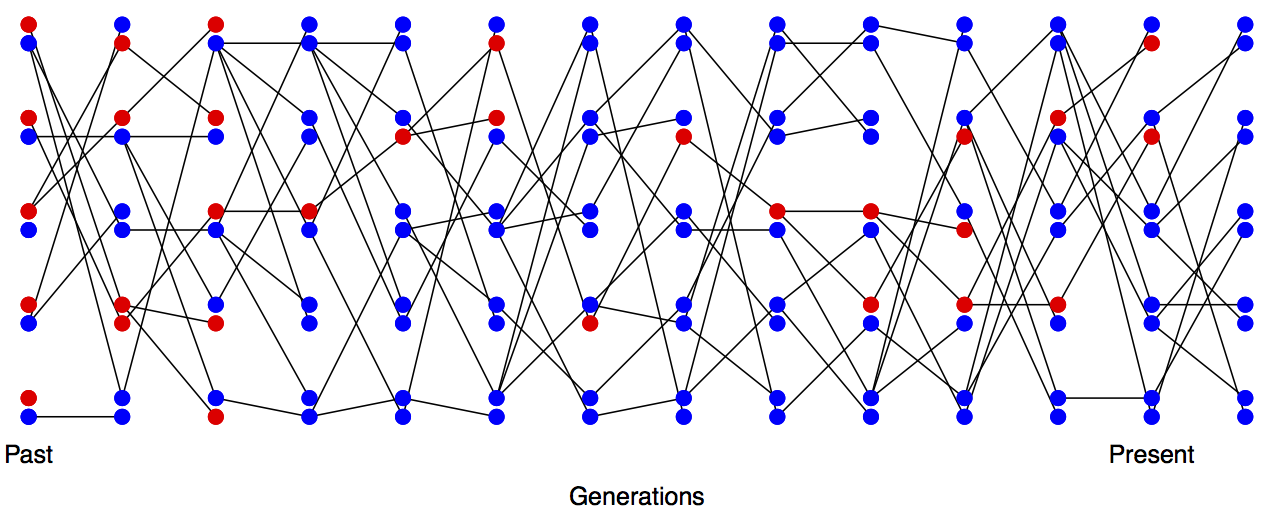
\includegraphics[width= \textwidth]{figures/Loss_of_he_col_two_alleles.png}
\end{center}
\caption{Loss of heterozygosity over time, in the absence of new
  mutations. A diploid population of 5 individuals over the
  generations, with lines showing transmission. In the first
  generation every individual is a heterozygote. \gitcode{https://github.com/cooplab/popgen-notes/blob/master/Rcode/Loss_of_heterozyg_varying_pop.R} } \label{fig:LossHet_two_alleles}
\end{figure} 

\begin{figure}
\begin{center}
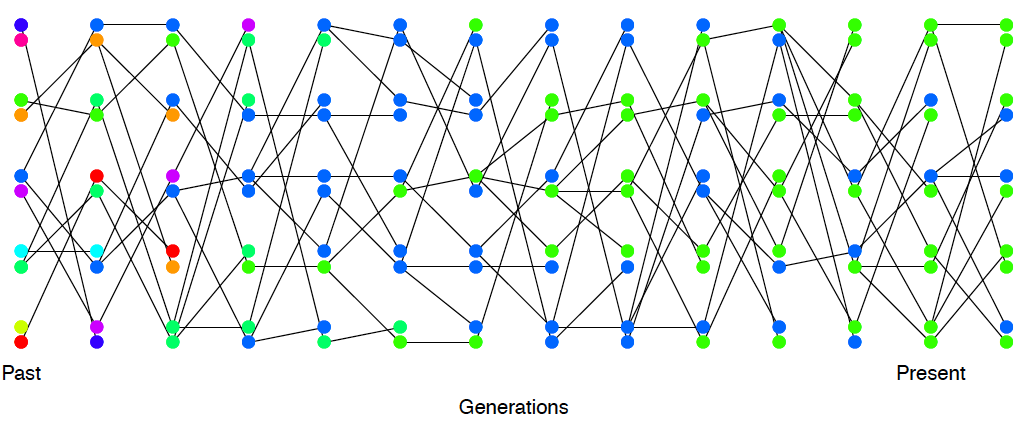
\includegraphics[width= \textwidth]{figures/Loss_of_het_2_many_alleles.png}
\end{center}
\caption{Loss of heterozygosity over time, in the absence of new
  mutations. A diploid population of 5 individuals. In the first generation I colour every allele a different
colour so we can track their descendants. \gitcode{https://github.com/cooplab/popgen-notes/blob/master/Rcode/Loss_of_heterozyg_varying_pop.R} } \label{fig:LossHet_many_alleles}
\end{figure} 


In the next generation ($t+1$) we are looking at the alleles in the
offspring of generation $t$. If we randomly sample two alleles in generation
$t+1$ which had different parental alleles in generation $t$, that
is just like drawing two random alleles from generation $t$. So the
probability that these two alleles in generation $t+1$, that have
different parental alleles in generation $t$, are non-identical is
$H_t$. \\

Conversely, if the two alleles in our pair had the same parental allele in
the proceeding generation (i.e. the alleles are identical by descent
one generation back) then these two alleles must be identical (as we
are not allowing for any mutation). \\



In a diploid population of size $N$ individuals there are $2N$ alleles. The
probability that our two alleles have the same parental allele in the
proceeding generation is $\nicefrac{1}{(2N)}$ and the probability that they have
different parental alleles is is $1-\nicefrac{1}{(2N)}$. So by the above
argument, the expected heterozygosity in generation $t+1$ is
%
\begin{equation}
H_{t+1} = \frac{1}{2N} \times 0 + \left(1-\frac{1}{2N} \right)H_t
\end{equation}
%
Thus, if the heterozygosity in generation $0$ is $H_0$, our
expected heterozygosity in generation $t$ is
%
\begin{equation}
H_t = \left(1-\frac{1}{2N} \right)^tH_0  \label{eqn:loss_het_discrete}
\end{equation}
%
i.e. the expected heterozygosity within our population is decaying
geometrically with each passing generation. If we assume that $\nicefrac{1}{(2N)}
\ll 1$ then we can approximate this geometric decay by an exponential
decay (see Question \ref{geo_question} below), such that
%
\begin{equation}
H_t =H_{0} e^{ - \nicefrac{t}{(2N)} }
\end{equation}
%
i.e. heterozygosity decays exponentially at a rate
$\nicefrac{1}{(2N)}$.

In Figure \ref{fig:LossHet_WF_N50} we show trajectories through time for 40 independently simulated loci drifting in a population of 50 individuals. Each population was started from a frequency of $30\%$ some drift up and some drift down eventually being lost or fixed from the population, but on average, across simulations, the allele frequency doesn't change. We also track heterozygosity, you can see that heterozygosity sometimes goes up, and sometimes goes down, but on average we are loosing heterozygosity, and this rate of loss is well predicted by eqn. \eqref{eqn:loss_het_discrete}. 
\begin{figure}
\begin{center}
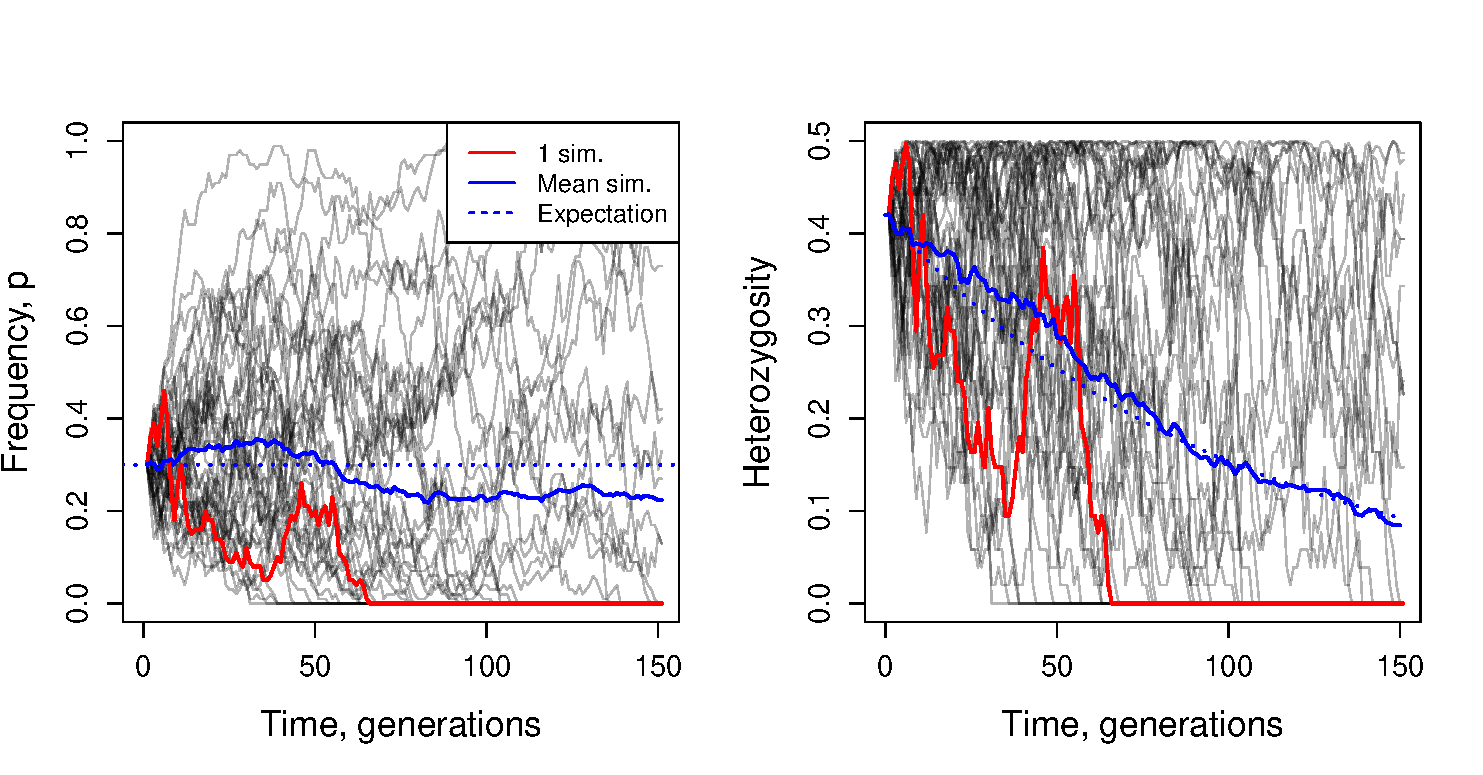
\includegraphics[width= \textwidth]{figures/WF_loss_het/WF_loss_het_N50.pdf}
\end{center}
\caption{Change in allele frequency and loss of heterozygosity over time for 40 replicates. Simulations of genetic drift in a diploid population of 50 individuals, in the absence of new mutations. We start 40 independent, biallelic loci each with an initial allele at 30\% frequency. The left panel shows the allele frequency over time and the right panel shows the heterozygosity over time, with the mean decay matching eqn. \eqref{eqn:loss_het_discrete}. \gitcode{https://github.com/cooplab/popgen-notes/blob/master/Rcode/Genetic_drift/WF_loss_of_het.R}} \label{fig:LossHet_WF_N50}
\end{figure} 


\begin{marginfigure}
\begin{center}
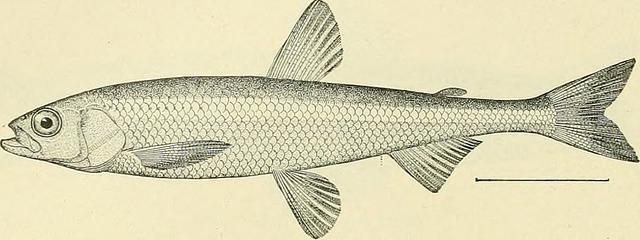
\includegraphics[width= \textwidth]{illustration_images/Genetic_drift/smelt/20497452375_9be855d9ff_z.jpg}
\end{center}
\caption{Pond smelt ({\it Hypomesus olidus}), a close relative of delta smelt. \BHLNC{Bulletin of the United States Fish Commission. 1906.}{https://archive.org/stream/bulletinofunited261906unit/\#page/270/mode/1up}{Smithsonian Libraries}} \label{fig:smelt}
\end{marginfigure} 

\begin{question} You are in charge of maintaining a population of delta smelt in the Sacramento river delta. Using a large set of microsatellites you
  estimate that the mean level of heterozygosity in this population is 0.005.
  You set yourself a goal of maintaining a level of heterozygosity of at least
  0.0049 for the next two hundred years. Assuming that the smelt have a
  generation time of 3 years, and that only genetic drift affects these loci, what is the smallest fully outbreeding population that you would need to maintain to meet this goal?  
\end{question}

Note how this picture of decreasing heterozygosity stands in contrast to the
consistency of Hardy-Weinberg equilibrium from the previous chapter. 
However, our Hardy-Weinberg \emph{proportions} still hold in forming each new generation. As the offsprings' genotypes in the next generation ($t+1$) represent a random
draw from the previous generation ($t$), if the parental frequency is $p_t$, we \emph{expect} a proportion $2p_t(1-p_t)$ of our offspring to be
heterozygotes (and HW proportions for our homozygotes). However, because population size is finite, the
observed genotype frequencies in the offspring will (likely) not match exactly with our expectations. As our genotype frequencies likely change slightly due
to sampling, biologically this reflects random variation in family size
and Mendelian segregation, the allele frequency will changed. Therefore, while each generation represents a sample from
Hardy-Weinberg proportions based on the generation before, our
genotype proportions are not at an equilibrium (an unchanging state) as the
underlying allele frequency changes over the generations. We'll develop some mathematical models for these allele
frequency changes later on. For now, we'll simply note that
under our simple model of drift (formally the Wright Fisher model), our
allele count in the $t+1^{th}$ generation represents a binomial sample
(of size $2N$) from the population frequency $p_t$ in the previous
generation.  If you've read to here, please email Prof Coop a picture of JBS Haldane in a striped suit with the title "I'm reading the chapter 3 notes''. (It's well worth googling JBS Haldane and to read more about his life; he's a true character and one of the last great polymaths. )

% generation $t$ may differ
%from that of $t+1$. We'll develop some mathematical models for these allele
%frequency changes 
 %from the previous generation we are
%drawing alleles at random from the  
%Here, the
%freqeuncy of each genotype will likely change, due to chance fluctuations in
%the underlying allele frequency $p$. While within a single generation
%Hardy--Weinberg proportions are maintained (at least approximately), across
%generations the genotypic frequencies change with allele frequency. The change
%in allele frequencies is due to drift: due to random variation in family size
%and Mendelian segregation, the allele frequency in generation $t$ may differ
%from that of $t+1$. We'll develop some mathematical models for these allele
%frequency changes later on.


\begin{marginfigure}[6cm]
\begin{center}
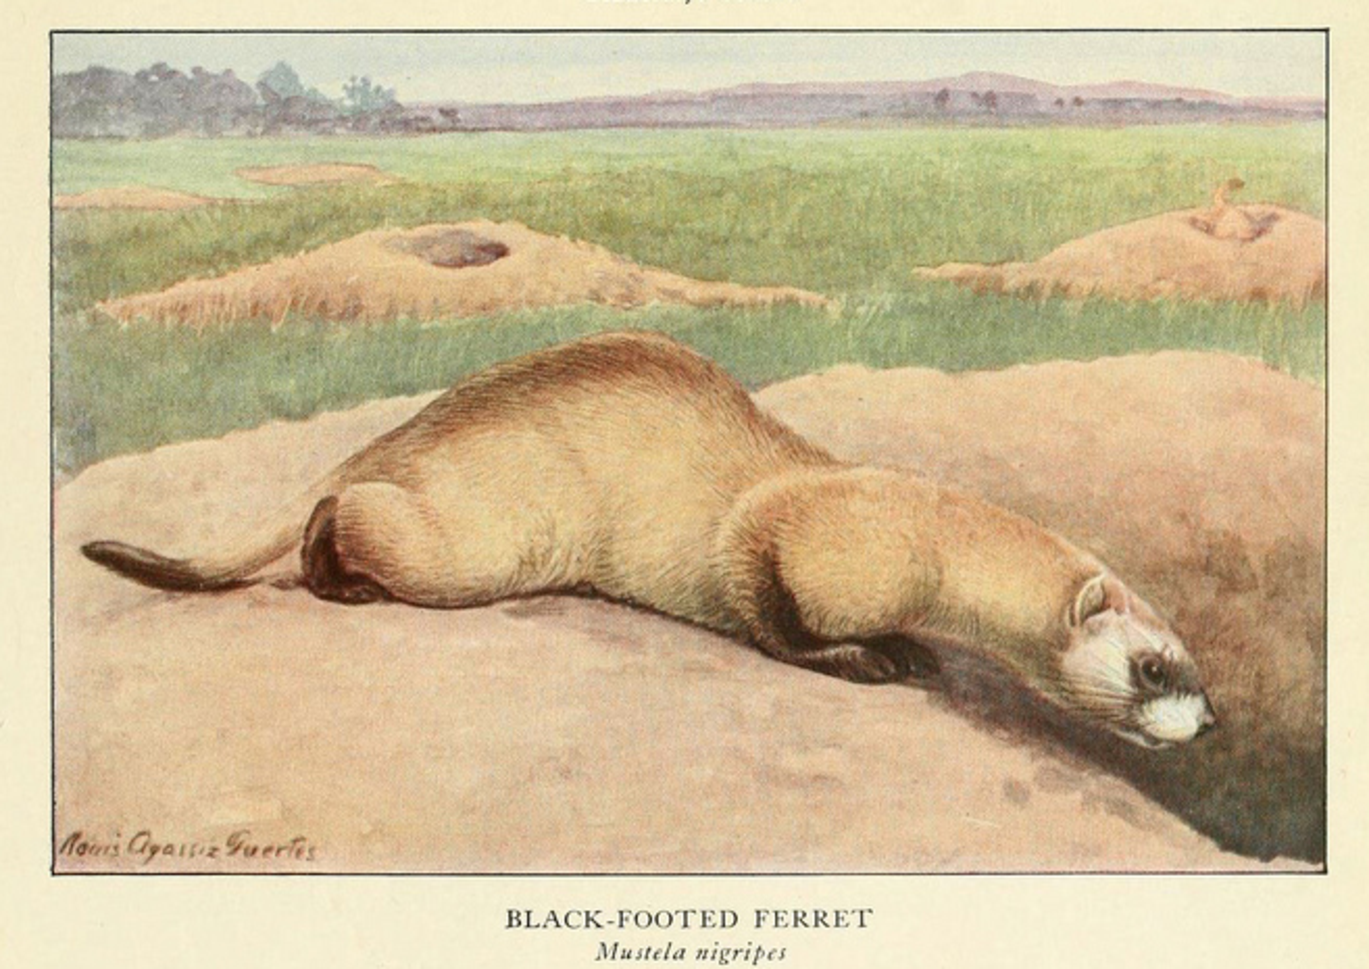
\includegraphics[width=\textwidth]{illustration_images/Genetic_drift/Black_footed_ferrets/Black_footed_ferret.pdf}
\end{center}
\caption{The black-footed ferret ({\it M. nigripes}). \BHLNC{Wild animals of North America, The National geographical
  society, 1918.}{https://www.biodiversitylibrary.org/page/9727900\#page/179/mode/1up}{American Museum of Natural History Library}} \label{fig:black_footed_ferret}  
\end{marginfigure} 

\begin{figure}
\begin{center}
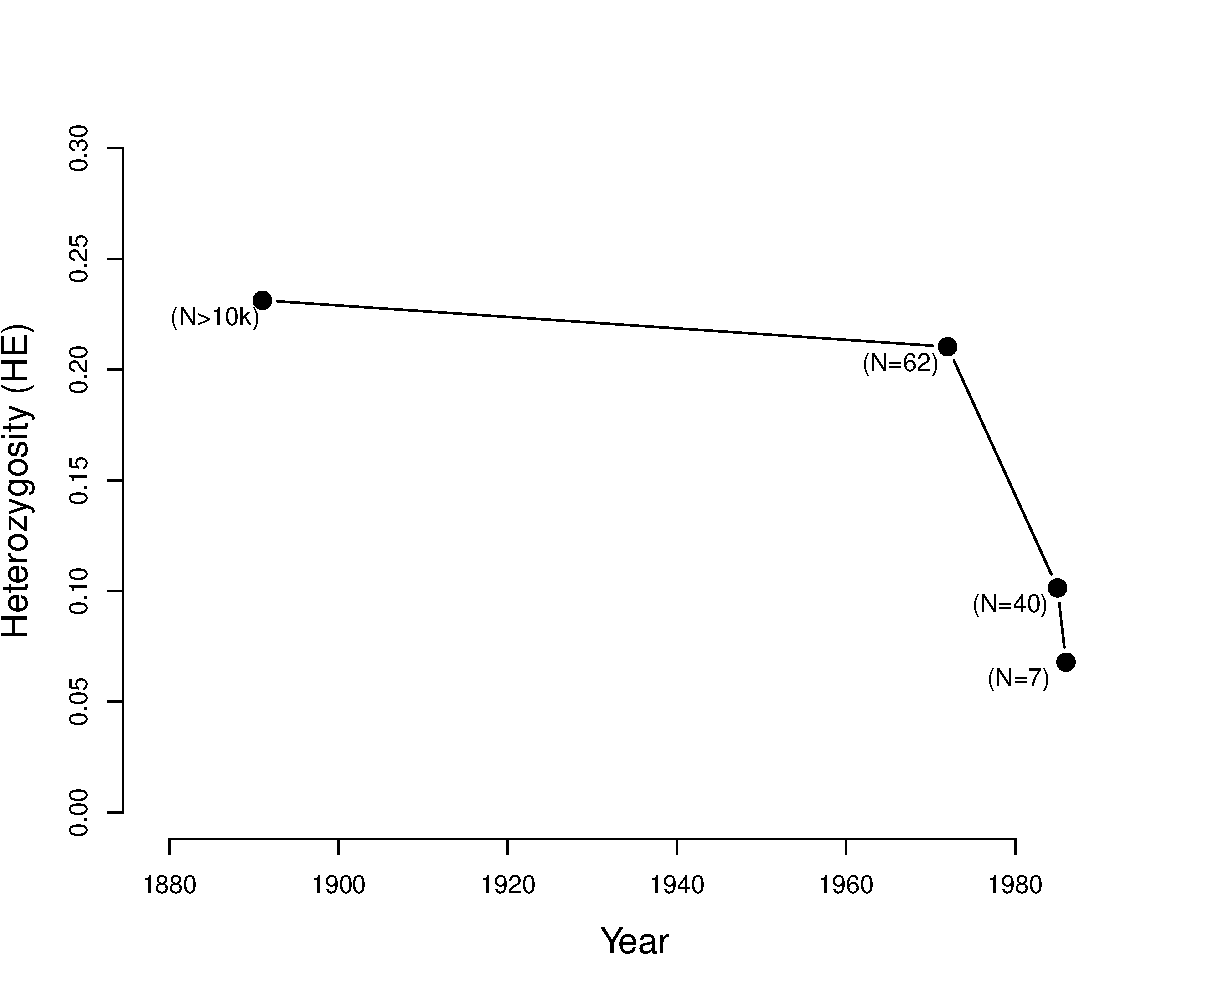
\includegraphics[width= \textwidth]{Journal_figs/genetic_drift/black_footed_ferrets/black_footed_ferrets_He.pdf}
\end{center}
\caption{Loss of heterozygosity in the Black-footed Ferrets in their declining population. Numbers in brackets give estimated number of individuals alve at that time. Data from \citet{Wisely:02}. \gitcode{https://github.com/cooplab/popgen-notes/blob/master/Journal_figs/genetic_drift/black_footed_ferrets/black-footed-ferrets_He.R}} \label{fig:LossHet_ferrets}  
\end{figure} 

To see how a decline in population size can affect levels of
heterozygosity, let's consider the case of black-footed ferrets ({\it Mustela nigripes}). The black-footed ferret population has declined dramatically through the twentieth century due
to destruction of their habitat.  In 1979, when the last known black-footed ferret died in captivity, they were thought to be
extinct. In 1981, a very small wild population was rediscovered ($40$ individuals), but in 1985 this population 
suffered a number of disease outbreaks. All of the $18$ remaining wild individuals
were brought into captivity, 7 of which
reproduced. Thanks to intense captive breeding efforts and conservation work, a
wild population of over 300 individuals has been established
since. However, because all of these individuals are descended from
those 7 individuals who survived the bottleneck, diversity levels
remain low.  \citeauthor{Wisely:02} measured heterozygosity at a number
of microsatellites in individuals from museum collections, showing the sharp drop in diversity as population sizes crashed (see Figure \ref{fig:LossHet_ferrets}).

\begin{question} \label{geo_question} In mathematical population genetics, a
  commonly used approximation is $(1-x) \approx e^{-x}$ for $x << 1$ (formally,
  this follows from the Taylor series expansion of $\exp(-x)$, ignoring second
  order and higher terms of $x$).  This approximation is especially useful for approximating a geometric
  decay process by an exponential decay process, e.g. $(1 - x)^t \approx e^{-xt}$. Using your calculator, or R, check how good of an approximation this is compared to the exact expression for two values of x, $x = 0.1$, and $0.01$, across two different values of t, $t=5$ and $t=50$. I.e. calculate both expressions for these values, hand in your answers and briefly comment on your results. 
 
  %Do this by plotting the geometric decay as
 % points, and the exponential decay as a curve, using different colors for each
 % of these three values of x. Note that you should have a discrete timescale for the
 % geometric decay (e.g. using \texttt{t=seq(0, 18)}) and a near continuous scale
 % for the exponential decay (e.g. using \texttt{t=seq(0, 18, length.out=100)}.
%  Print off your graph and hand it in with your homework. 
    % max <- 18; x <- seq(0, max); x1 <- seq(0, max, length.out=100); plot(x, (1-0.5)^x, col='purple', pch=19); lines(x1, exp(-0.5*x1), col='purple'); points(x, (1-0.1)^x, pch=19, col='orange'); lines(x1, exp(-0.1*x1), col='orange'); points(x, (1-0.01)^x, pch=19, col='green'); lines(x1, exp(-0.01*x1), col='green') # messy but works
\end{question}

\subsection{Levels of diversity maintained by a balance between
 mutation and drift} \label{DriftMutationBalance}

Next we're going to consider the amount of neutral polymorphism that can be maintained in a population as a balance between genetic drift removing variation and mutation introducing new neutral variation, see Figure \ref{fig:Mut_Sel_balance} for an example. Note in our example, how no-one allele is maintained at a stable equilibrium, rather an equilibrium level of polymorphism is maintained by a constantly shifting case of alleles. 

\begin{figure} \begin{center} 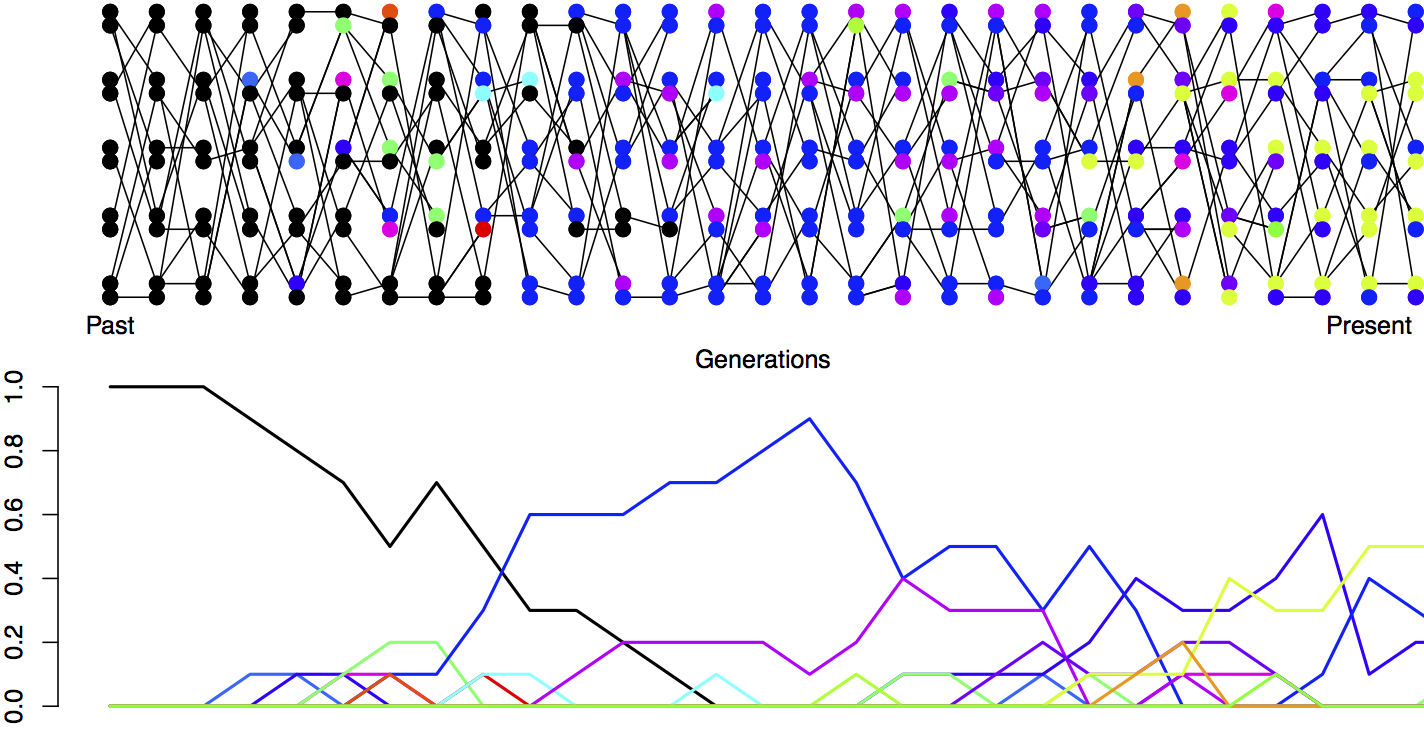
\includegraphics[width= 0.8
\textwidth]{figures/Mut_drift_balance.png} \end{center} \caption{Mutation-drift
balance. A diploid population of 5 individuals. In the first generation
everyone has the same allele (black). Each generation the transmitted allele
can mutate and we generate a new colour. In the bottom plot, I trace the
frequency of alleles in our population over time. The mutation rate we use is very high, simply to maintain diversity in this small population. \gitcode{https://github.com/cooplab/popgen-notes/blob/master/Rcode/Loss_of_heterozyg_varying_pop.R}} \label{fig:Mut_Sel_balance}
\end{figure} 

\paragraph{The neutral mutation rate.} 
We'll first want to consider the rate at which neutral mutations arise in the population.Thinking back to our discussion of the neutral theory of molecular evolution, let's suppose that there are only two classes of mutation that can arise in our genomic region of interest: neutral mutations and highly deleterious mutations. The total mutation rate at our locus is $\mu_T$ per generation, i.e. per transmission from parent to child. A fraction $C$ of our mutations are new alleles that are highly deleterious and so quickly removed from the population. We'll call this $C$ parameter the constraint, and it will differ according to the genomic region we consider.  The remaining fraction $(1-C)$ are our neutral mutations, such that our neutral mutation rate is 
\begin{equation}
\mu = (1-C) \mu_T
\end{equation}
This is the per generation rate.

\begin{question}
It's worth taking a minute to get familiar with both how rare, and how common, mutation is. The per base pair mutation rate in humans is around $1.5 \times 10^{-8}$ per generation. That means, on average, we have to monitor a site for $\sim 66.6$ million transmissions from parent to child to see a mutation. Yet populations and genomes are big places, so mutations are common at these levels. \\
{\bf A)} Your autosomal genome is $\sim 3$ billion base pairs long ($3 \times 10^9$). You have two copies, the one you received from your mum and one from your dad. What is the average (i.e. the expected) number of mutations that occurred in the transmission from your mum and your dad to you?\\
{\bf B)} The current human population size is $\sim 7$ billion individuals. How many times, at the level of the entire human population, is a single base-pair mutated in the transmission from one generation to the next? 
\end{question}
\paragraph{Levels of heterozygosity maintained as a balance between mutation and selection.}


Looking backwards in time from one generation to the previous generation, we are going to say that two alleles which have the same parental allele (i.e. find their common ancestor) in the preceding generation have \emph{coalesced}, and refer to this
event as a \emph{coalescent event}.

The probability that our pair of randomly sampled alleles have coalesced in the
preceding generation is $\nicefrac{1}{(2N)}$, the probability that our pair of
alleles fail to coalesce is $1-\nicefrac{1}{(2N)}$. 

The probability that a mutation changes the identity of the
transmitted allele is $\mu$ per generation. So the probability of no
mutation occurring is $(1-\mu)$. We'll assume that when a mutation
occurs it creates some new allelic type which is not present in the
population. This assumption (commonly called the infinitely-many-alleles model) makes the math slightly cleaner, and also
is not too bad an assumption biologically. See Figure
\ref{fig:Mut_Sel_balance} for a depiction of mutation-drift balance in
this model over the generations.

This model lets us calculate when our two alleles last shared a common
ancestor and whether these alleles are identical as a result of
failing to mutate since this shared ancestor.  For example, we can work out the probability that our
two randomly sampled alleles coalesce $2$ generations in the past
(i.e. they fail to coalesce in generation $1$ and then coalesce in
generation $2$), and
that they are identical as
\begin{equation}
\left(1- \frac{1}{2N} \right) \frac{1}{2N} (1-\mu)^4
\end{equation}
Note the power of $4$ is because our two alleles have to have failed
to mutate through $2$ meioses each. 

More generally, the probability that our alleles coalesce in generation
$t+1$ (counting backwards in time) and are identical due to no mutation to either allele in the
subsequent generations is
%
\begin{equation}
P(\textrm{coal. in t+1 \& no mutations}) =  \frac{1}{2N} \left(1- \frac{1}{2N} \right)^t \left(1-\mu \right)^{2(t+1)}
\end{equation}
%
To make this slightly easier on ourselves let's further assume that $t
\approx t+1$ and so rewrite this as:
\begin{equation}
P(\textrm{coal. in t+1 \& no mutations}) \approx \frac{1}{2N} \left(1- \frac{1}{2N} \right)^t \left(1-\mu \right)^{2t}
\end{equation}
%

This gives us the approximate probability that two alleles will coalesce in the
$(t+1)^\text{th}$ generation. In general, we may not know when two alleles may
coalesce: they could coalesce in generation $t=1, t=2, \ldots $, and so on.
Thus, to calculate the probability that two alleles coalesce in \emph{any}
generation before mutating, we can write:

\begin{align*}
  P(\textrm{coal. in any generation \& no mutations}) \approx & P(\textrm{coal. in} \; t=1 \; \textrm{\& no mutations}) \; + \\ 
&  P(\textrm{coal. in} \; t=2 \; \textrm{\& no mutations}) + \ldots \\
  %P(\textrm{coal. in} \; t=3 \; \textrm{\& no mutations})  +\ldots \\
  = & \sum_{t=1}^\infty P(\textrm{coal. in } \; t \; \textrm{generations \& no mutation})
\end{align*}
%
which follows from basic probability and the fact that coalescing in a particular generation is mutually exclusive with coalescing in a different generation.

While we could calculate a value for this sum given $N$ and $\mu$, it's
difficult to get a sense of what's going on with such a complicated expression.
Here, we turn to a common approximation in population genetics (and all applied
mathematics), where we assume that $\nicefrac{1}{(2N)} \ll 1$ and $\mu \ll 1$.
This allows us to approximate the geometric decay as an exponential decay.
Then, the probability two alleles coalesce in generation $t+1$ and don't mutate
can be written as:
%
\begin{align} P(\textrm{coal. in t+1 \& no mutations}) &\approx \frac{1}{2N}
\left(1- \frac{1}{2N} \right)^t \left(1-\mu \right)^{2t} \\ 
& \approx \frac{1}{2N} e^{-t/(2N)} e^{-2\mu t } \\
&=\frac{1}{2N} e^{-t(2\mu+1/(2N))} \end{align} 
%
Then we can approximate the summation by an integral, giving us:
%

\begin{equation}
\frac{1}{2N} \int_0^{\infty} e^{-t(2\mu+1/(2N))} dt =
\frac{1/(2N)}{1/(2N)+2\mu} = \frac{1}{1+4N\mu}
\end{equation}

The equation above gives us the probability that our two alleles coalesce at some point
in time, and do not mutate before reaching their common
ancestor. Equivalently, this can be thought of as the probability our two
alleles coalesce \emph{before} mutating, i.e. that they are homozygous. 

Then, the complementary probability that our pair of alleles are non-identical
(or heterozygous) is simply one minus this. The following equation gives the equilibrium
heterozygosity in a population at equilibrium between mutation and drift:

\marginnote{This result was derived by \citet{kimura1964number} and \citet{malecot:48}  \citep[see][for an English translation, the lack of earlier translation meant this result was missed]{malecot:69}. Technically we're assuming that every new mutation creates a new allele, the so-called "infinitely many alleles" model, otherwise our pair of sequences could be identical due to repeat or back mutation. See this GENETICS \href{http://genestogenomes.org/kimura-crow-infinite-alleles/}{blog post} and \citet{ewens2016motoo} for a nice discussion of the history. }

\begin{equation}
  H = \frac{4N\mu}{1+4N\mu} \label{eqn:hetero}
\end{equation}
 compound parameter $4N\mu$, the population-scaled mutation rate,
will come up a number of times so we'll give it its own name:
\begin{equation}
\theta = 4N\mu
\end{equation}

So all else being equal, species with larger population sizes should
have proportionally higher levels of neutral polymorphism.  

\begin{question}
The sequence-level heterozygosity in {\it Capsella grandiflora} (grand shepherd's purse) is $\sim 2\%$ per base. Assuming a mutation rate of $10^{-9} bp^{-1}$ per generation, what is your estimate of the population size of {\it C. grandiflora}?  
\end{question}

\subsection{The effective population size}
\marginnote{the effective population size ($N_e$) is the population size that
would result in the same rate of drift in an idealized population of constant size (following our modeling
assumptions)
as that observed in our true population .}

In practice, populations rarely conform to our assumptions of being constant in size with low variance in reproductive success. Real populations experience dramatic fluctuations in size, and there is
often high variance in reproductive success. Thus rates of drift in
natural populations are often a lot higher than the census population
size would imply. See Figure \ref{fig:LossHet_varying_pop}  for a depiction of
a repeatedly bottlenecked population losing diversity at a fast rate.

\begin{figure}
\begin{center}
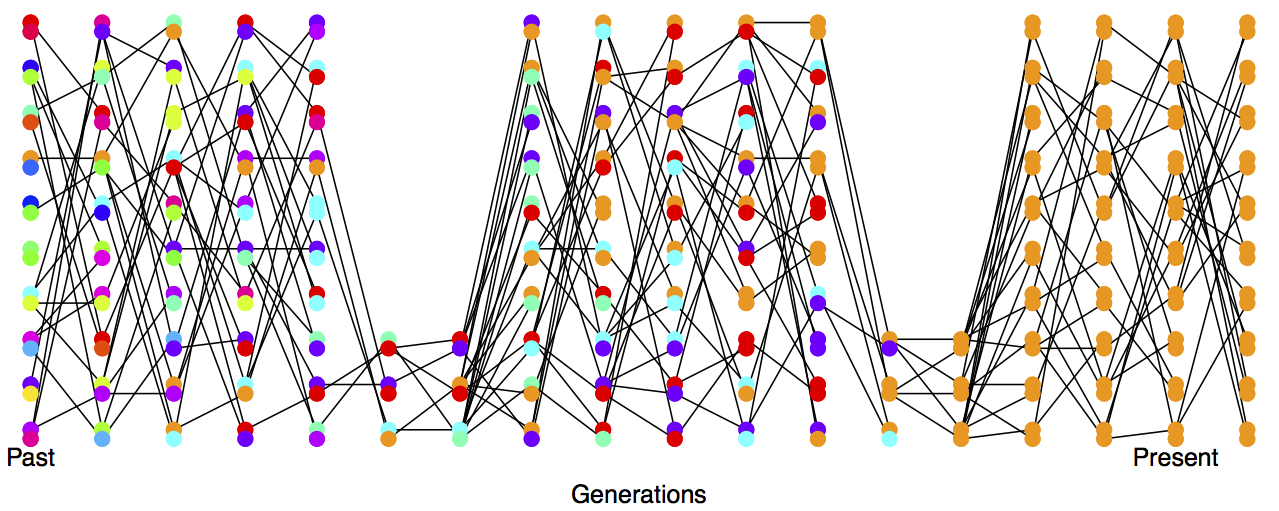
\includegraphics[width= \textwidth]{figures/Loss_of_he_col_alleles_varying_pop_dark.png}
\end{center}
\caption{Loss of heterozygosity over time in a bottlenecking population. A diploid population of 10 individuals, that bottlenecks
  down to three individuals repeatedly. In the first generation, I colour every allele a different
colour so we can track their descendants. There are no new
  mutations. \gitcode{https://github.com/cooplab/popgen-notes/blob/master/Rcode/Loss_of_heterozyg_varying_pop.R}} \label{fig:LossHet_varying_pop}  
\end{figure} 


To cope with this discrepancy, population geneticists often invoke the concept of
an \emph{effective population size} ($N_e$). In many situations (but not all), departures from model assumptions can be captured by substituting $N_e$ for $N$.
\\


If population sizes vary rapidly in size, we can (if certain conditions are met) replace our population size by the harmonic mean population size.
Consider a diploid population of variable size, whose size is $N_t$ $t$ generations into the
past. The probability our pairs of alleles have not coalesced by generation $t$ is
given by
\begin{equation}
\prod_{i=1}^{t} \left(1-\frac{1}{2N_i} \right) \label{eqn:var_pop_coal}
\end{equation}
Note that this simply collapses to our original expression
$\left(1-\frac{1}{2N } \right)^t $ if $N_i$ is constant. Under this model, the rate of loss of heterozygosity in this population is equivalent to
a population of effective size
\begin{equation}
N_e =\frac{1}{\frac{1}{t} \sum_{i=1}^{t} \frac{1}{N_i} }. \label{eq:Ne_harmonic}
\end{equation}
This is the harmonic mean of the varying population size. \sidenote[][-6cm]{
To see this, note that if $1/(N_i)$ is
small, then we can approximate \eqref{eqn:var_pop_coal} using the exponential approximation: 
\begin{equation}
\prod_{i=1}^{t} \exp \left( -\frac{1}{2N_i} \right)   =
\exp \left(- \sum_{i=1}^{t} \frac{1}{2N_i} \right) .
\end{equation}
When we put the product inside the exponent, it becomes a sum.  We can also write the probability of not coalescing by generation $t$ in a population of constant size ($N_e$) as an exponential, so that it takes the same form as the expression above on the right. Comparing the exponent in the two cases, we see
\begin{equation}
\frac{t}{2N_e} = \sum_{i=1}^{t} \nicefrac{1}{2N_i} 
\end{equation}
So that if we want a constant effective population size ($N_e$) that has the same
rate of loss of heterozygosity as our variable population, we need to rearrange and solve this equation to give \eqref{eq:Ne_harmonic}. }


Thus our effective population size, the size of an idealized constant
population which matches the rate of genetic drift, is the harmonic
mean true population size over time. The harmonic mean is very
strongly affected by small values, such that if our population size is
one million $99\%$ of the time but drops to $1000$ every hundred or
so generations, $N_e$ will be much closer to $1000$ than a
million. \\


%would result in the same rate of drift
%Luckily, in many (not all) situations, departures from model assumptions can be captured by substituting Ne for N, i.e., by plugging in a fictitious N that leads to the same level of genetic drift as observed.

\begin{figure}
\begin{center}
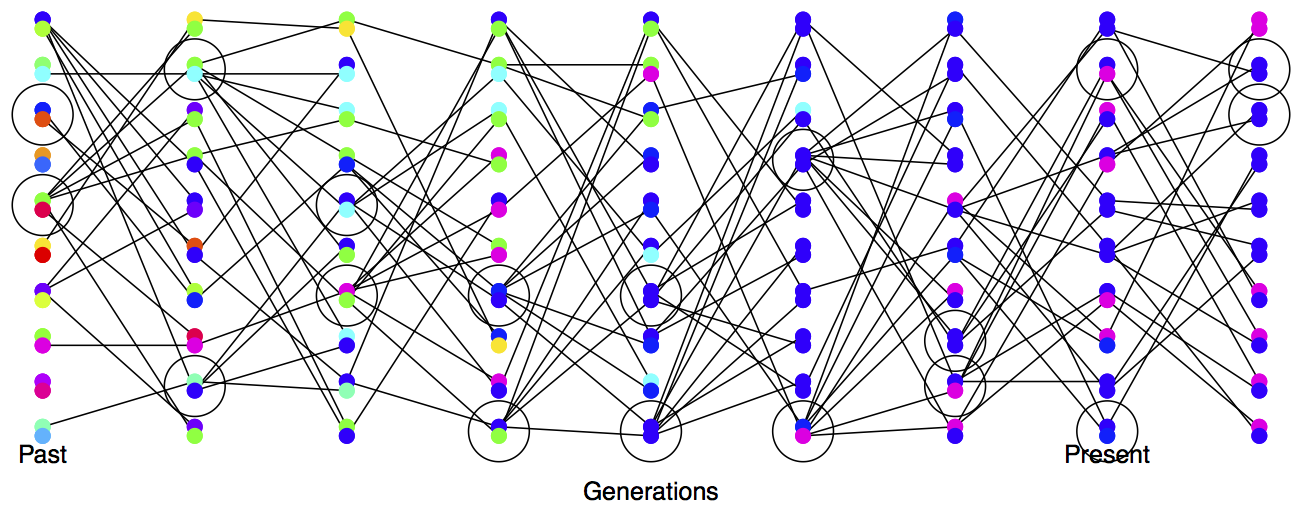
\includegraphics[width= \textwidth]{figures/Loss_of_he_col_alleles_varying_RS.png}
\end{center}
\caption{High variance on reproductive success increases the rate of genetic drift. A diploid population of 10 individuals, where the circled
  individuals have much higher reproductive success. In the first generation I colour every allele a different
colour so we can track their descendants, there are no new
  mutations. \gitcode{https://github.com/cooplab/popgen-notes/blob/master/Rcode/Loss_of_heterozyg_varying_pop.R}} \label{fig:LossHet_varying_RS}
\end{figure} 

Variance in reproductive success will also affect our effective
population size. Even if our population has a large constant size $N$
individuals, if only small proportion of them get to reproduce, then
the rate of drift will reflect this much smaller number of reproducing
individuals. See Figure \ref{fig:LossHet_varying_RS} for a depiction of the higher rate of drift
in a population where there is high variance in reproductive success.

To see one example of this, consider the case where $N_F$ of  females get to reproduce and $N_M$ males get reproduce.
While every individual has a mother an a father, not every individual gets to be a parent. In practice, in many animal species far more females get to reproduce than males, i.e. $NM <N_F$, as a few males get many mating opportunities and many males get no/few mating opportunities \citep[see ][for a broad analysis, and note that there a certainly many exceptions to this general pattern]{janicke:16}. When our two alleles pick an ancestor, $25\%$ of the time our alleles were both in a female ancestor, in which case they are IBD with probability $1/(2N_F)$, and $25\%$ of the time they are both in a
male ancestor, in which case they coalesce with probability
$1/(2N_M)$. The remaining $50\%$ of the time, our alleles trace back to two individuals of different sexes in the prior generation and so cannot coalesce.  Therefore, our probability of coalescence in the preceding generation is 
\begin{equation}
\frac{1}{4}\left(\frac{1}{2N_M} \right)+\frac{1}{4}\left(\frac{1}{2N_F} \right) %=
%\frac{1}{8}\frac{N_F+N_M}{N_FN_M} 
\end{equation}
i.e. the rate of coalescence is the harmonic mean of the two sexes' population sizes, equating this to $\frac{1}{2N_e}$ we find

\begin{marginfigure}
\begin{center}
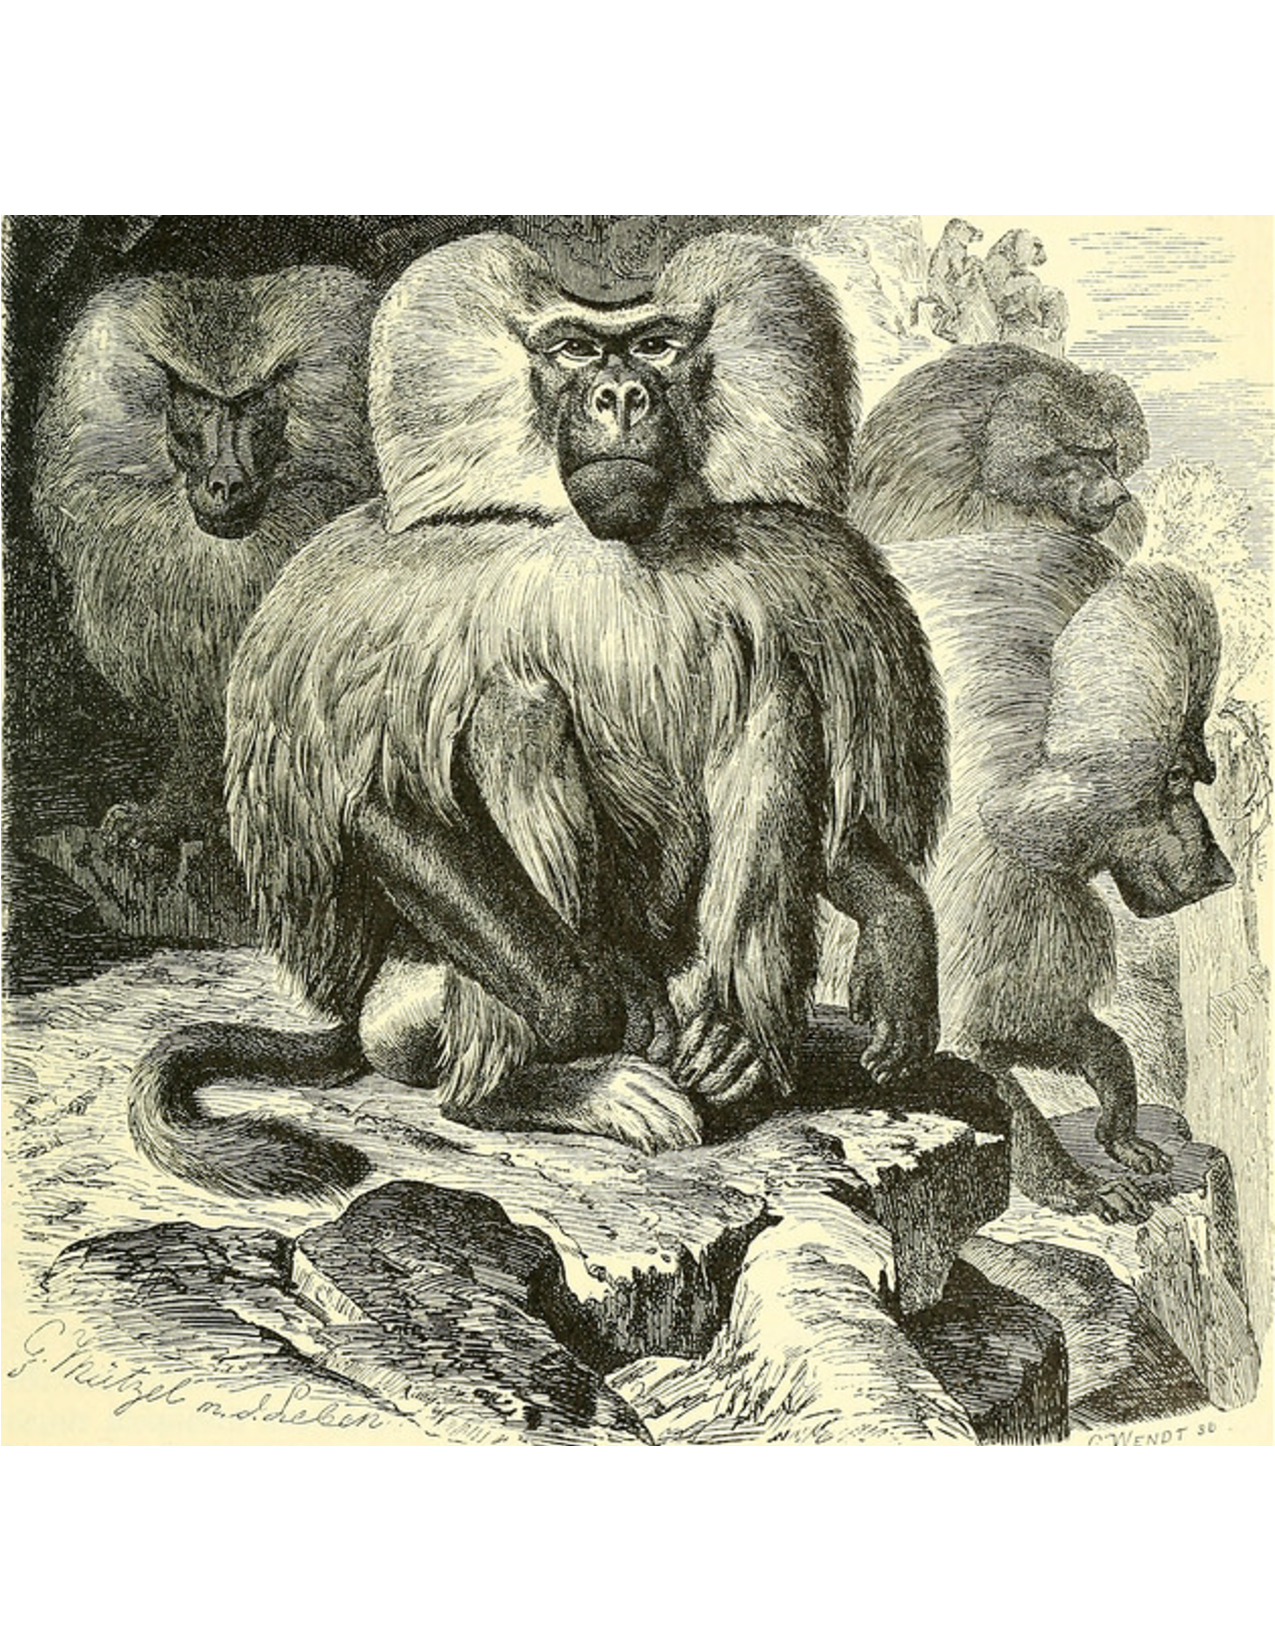
\includegraphics[width= 0.7 \textwidth]{illustration_images/Genetic_drift/Hamadryas_baboon/Hamadryas_baboon.pdf}
\end{center}
\caption{Male Hamadryas baboons. Up to ten females live in a harem with a single male.\BHLNC{Brehm's Tierleben (Brehm's animal life). Brehm,
  A.E. 1893.}{https://archive.org/stream/brehmstierlebena001breh/\#page/181/mode/1up}{University of Illinois Urbana-Champaign}  %Brehm's animal life
} \label{fig:Hamadryas_baboon}  
\end{marginfigure} 

\begin{equation}
N_e = \frac{4N_FN_M}{N_F+N_M}
\end{equation}
Thus if reproductive success is very skewed in one sex (e.g. $N_M \ll
N/2$), our effective population size will be much reduced as a result. For more on how different evolutionary forces affect the rate of genetic drift, and their impact on the effective population size, see \citet{charlesworth:09}.\\

\begin{question}
You are studying a population of 500 males and 500 females Hamadryas baboons. Assume that all of the females but only 1/10 of the males get to mate: 
{\bf A)} What is the effective population size for the autosome?\\
{\bf B)} Do you expect the {\it ratio} of X-chromosome to autosomal diversity to be higher or lower in this species compared to a species where the sexes have more similar variance in reproductive success? Explain the intuition behind your answer.
 \end{question}

\graham{Add X chromosome Ne?}
\section{The Coalescent and patterns of neutral diversity}

\begin{quote}
"Life can only be understood backwards; but it must be lived
forwards." -- Kierkegaard
\end{quote}

\paragraph{Pairwise Coalescent time distribution and the number of
 pairwise differences.}
Thinking back to our calculations we made about the loss of neutral heterozygosity
and equilibrium levels of diversity (in Sections \ref{LossofHet} and \ref{DriftMutationBalance}), you'll note that we could first specify
which generation a pair of sequences coalesce in, and then calculate
some properties of heterozygosity based on that. That's because neutral
mutations do not affect the probability that an individual transmits
an allele, and so don't affect the way in which we can trace ancestral lineages
back through the generations. \\


As such, it will often be helpful to consider the time to the common
ancestor of a pair of sequences, and then think of the impact of that time to coalescence
on patterns of diversity. See Figure \ref{fig:Coalescent_simulation}
for an example of this. 

\begin{figure}
\begin{center}
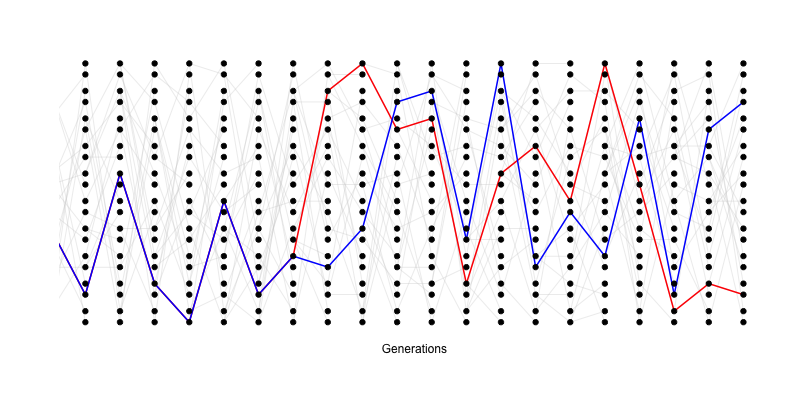
\includegraphics[width=\textwidth]{figures/Coalescent.png}
\end{center}
\caption{A simple simulation of the coalescent process. The simulation
  consists of a diploid population of 10 individuals (20 alleles). In
  each generation, each individual is equally likely to be the parent
  of an offspring (and the allele transmitted is indicated by a light
  grey line).  We track a
  pair of alleles, chosen in the present day, back 14 generations
  until they find a common ancestor. \gitcode{https://github.com/cooplab/popgen-notes/blob/master/Rcode/track_alleles.R} } \label{fig:Coalescent_simulation}  %https://github.com/cooplab/popgen-notes/blob/master/Rcode/track_alleles.R
\end{figure}

The probability that a pair of alleles
have failed to coalesce in $t$ generations and then coalesce in the
$t+1$ generation back is 
\begin{equation}
 P(T_2=t+1) = \frac{1}{2N} \left(1- \frac{1}{2N} \right)^{t} \label{eqn:coal_time_dist}
\end{equation}
Thus the coalescent time of our pair of alleles is a Geometrically distributed random variable, where the probability of success is $1/(2N)$; we denote this by $T_2 \sim  \text{Geo}(1/(2N))$.
The expected (i.e. the mean over many replicates) coalescent time of a pair of alleles is then  
\begin{equation}
\E(T_2) = 2N 
\end{equation}
generations.\\

\marginnote{Blurring our eyes a little, we can see  that \ref{eqn:coal_time_dist} is
\begin{equation}
\approx \frac{1}{2N} e^{-t/(2N)} 
\end{equation}
and so think of  a continuous random variable, i.e. we could say that the coalescent time of a pair of sequences ($T_2$) is approximately exponentially distributed with a rate $1/(2N)$, i.e. $T_2 \sim \text{Exp}\left( 1/(2N) \right)$. Formally we can do this by taking the limit of the discrete process more carefully. }

Conditional on a pair of alleles coalescing $t$ generations ago,
there are $2t$ generations in which a mutation could occur. If the per
generation mutation rate is $\mu$, then the expected number of
mutations between a pair of alleles coalescing $t$ generations ago is
$2 t\mu$ (the alleles have gone through a total of $2t$ meioses since they last shared a common ancestor). So we can write the expected
number of mutations ($S_2$) separating two alleles drawn at random from the
population as %\erin{I added subscript 2 to all the T's, which I think is appropriate}
\begin{align}
\E(S_2) &= \sum_{t=0}^{\infty} \E(S_2 | T_2=t) P(T_2=t) \nonumber\\
& =\sum_{t=0}^{\infty} 2 \mu t P(T_2=t) \nonumber\\
& =2\mu \E(T_2)  \nonumber\\
& = 4 \mu N 
\end{align}
 
%As our expected coalescent time is $2N$ generations (which follows from the expected value of exponential distributions), the expected
%number of mutations separating two alleles drawn at random from the
%population is
%
%\begin{align}
 % \E(j) &= 2\mu\E(t) \\ \nonumber
 % &= 4N\mu \\
 % &= \theta \nonumber
%\end{align}
We'll assume that mutation is rare enough that it never happens at the same basepair twice, i.e. no multiple hits, such that we get to see all of the mutation events that separate our pair
of sequences \sidenote{This is called the infinitely-many-sites assumption,
which should be fine if $N\mu_{BP} \ll 1$, where $\mu_{BP}$ is the mutation rate per base pair).} Thus the number of
mutations between a pair of sites is the observed number of
differences between a pair of sequences. In the previous chapter we denote the observed number of pairwise differences at putatively neutral
sites separating a pair of sequences as $\pi$ (we usually average this over a
number of pairs of sequences for a region). Therefore, under our simple, neutral, constant population-size model we expect
\begin{equation}
\E(\pi) = 4 N \mu = \theta
\end{equation}
So we can get an empirical estimate of $\theta$ from
$\pi$, let's call this $\widehat{\theta}_{\pi}$, by setting $\widehat{\theta}_{\pi}=\pi$., i.e. our observed level of pairwise genetic diversity.  If we
have an independent estimate of $\mu$, then from setting $\pi =\widehat{\theta}_{\pi} = 4N\mu$ we can furthermore obtain an estimate of the population
size $N$ that is consistent with our levels of neutral polymorphism. If we estimate the population size this way, we should call it the effective coalescent population size ($N_e$). It's best to think about $N_{e}$ estimated from neutral diversity as a long-term, effective population size for the species, but there's a boat load of caveats that come along with that assumption. For example, past bottlenecks and population expansions are all subsumed into a single number and so this estimated $N_{e}$ may not be very representative of the population size at any time. That said, it's not a bad place to start when thinking about the rate of genetic drift for neutral diversity in our population over long time-periods. \sidenote{Up to this point we've been describing only neutral processes, however, selection can also alter levels of polymorphism. For example, if some synonymous sites directly experience selection, then even if we use $\pi$ calculated for on synonymous changes we may underestimate the coalescent effective population size. As we'll see later in the notes, selection at linked sites can also impact neutral diversity. As such, if we can, we may want to use genomic sites subject to the weakest selective constraints, and also far from gene-dense or otherwise very constrained regions of the genome, to estimate $N_e$ from $\pi$. But even then caution is warranted. } 

Lets take a moment to distinguish our expected heterozygosity (eqn. \ref{eqn:hetero}) from our expected number of pairwise differences ($\pi$). Our expected heterozygosity is the probability that two alleles at a locus, sampled from a population at random, are different from each other. If one or more mutations have occurred since a pair of alleles last shared a common ancestor, then our sequences will be different from each other. On the other hand, our $\pi$ measure keeps track of the average total number of differences between our loci. As such, $\pi$ is often a more useful measure, as it records the number of differences between the sequences, not just whether they are different from each other (however, for certain types of loci, e.g. microsatellites, heterozygosity is often used as we cannot usually count up the minimum number of mutations in a sensible way). In the case where our locus is a single basepair, the two measures will usually be close to one another, as $H \approx \theta$ for small values of $\theta$. For example, comparing two sequences at random in humans, $\pi \approx 1/1000$ per basepair, and the probability that a specific base pair differs between two sequences is $\approx 1/1000$. However, these two quantities start to differ from each other when we consider regions with higher mutation rates. For example, if we consider a 10kb region, our mutation rate will 10,000 times larger than a single base pair. For this length of sequence the probability that two randomly chosen haplotypes differ is quite different from the number of mutational differences  between them. (Try a mutation rate of $10^{-8}$ per base and a population size of $10,~000$ in our calculations of $\E[\pi]$ and H to see this.)

%\erin{can you give an intuitive example when per bp $\pi$ is very different from heterozygosity? Or is this distinction really just key when we're talking about larger loci?}

\begin{marginfigure}
\begin{center}
  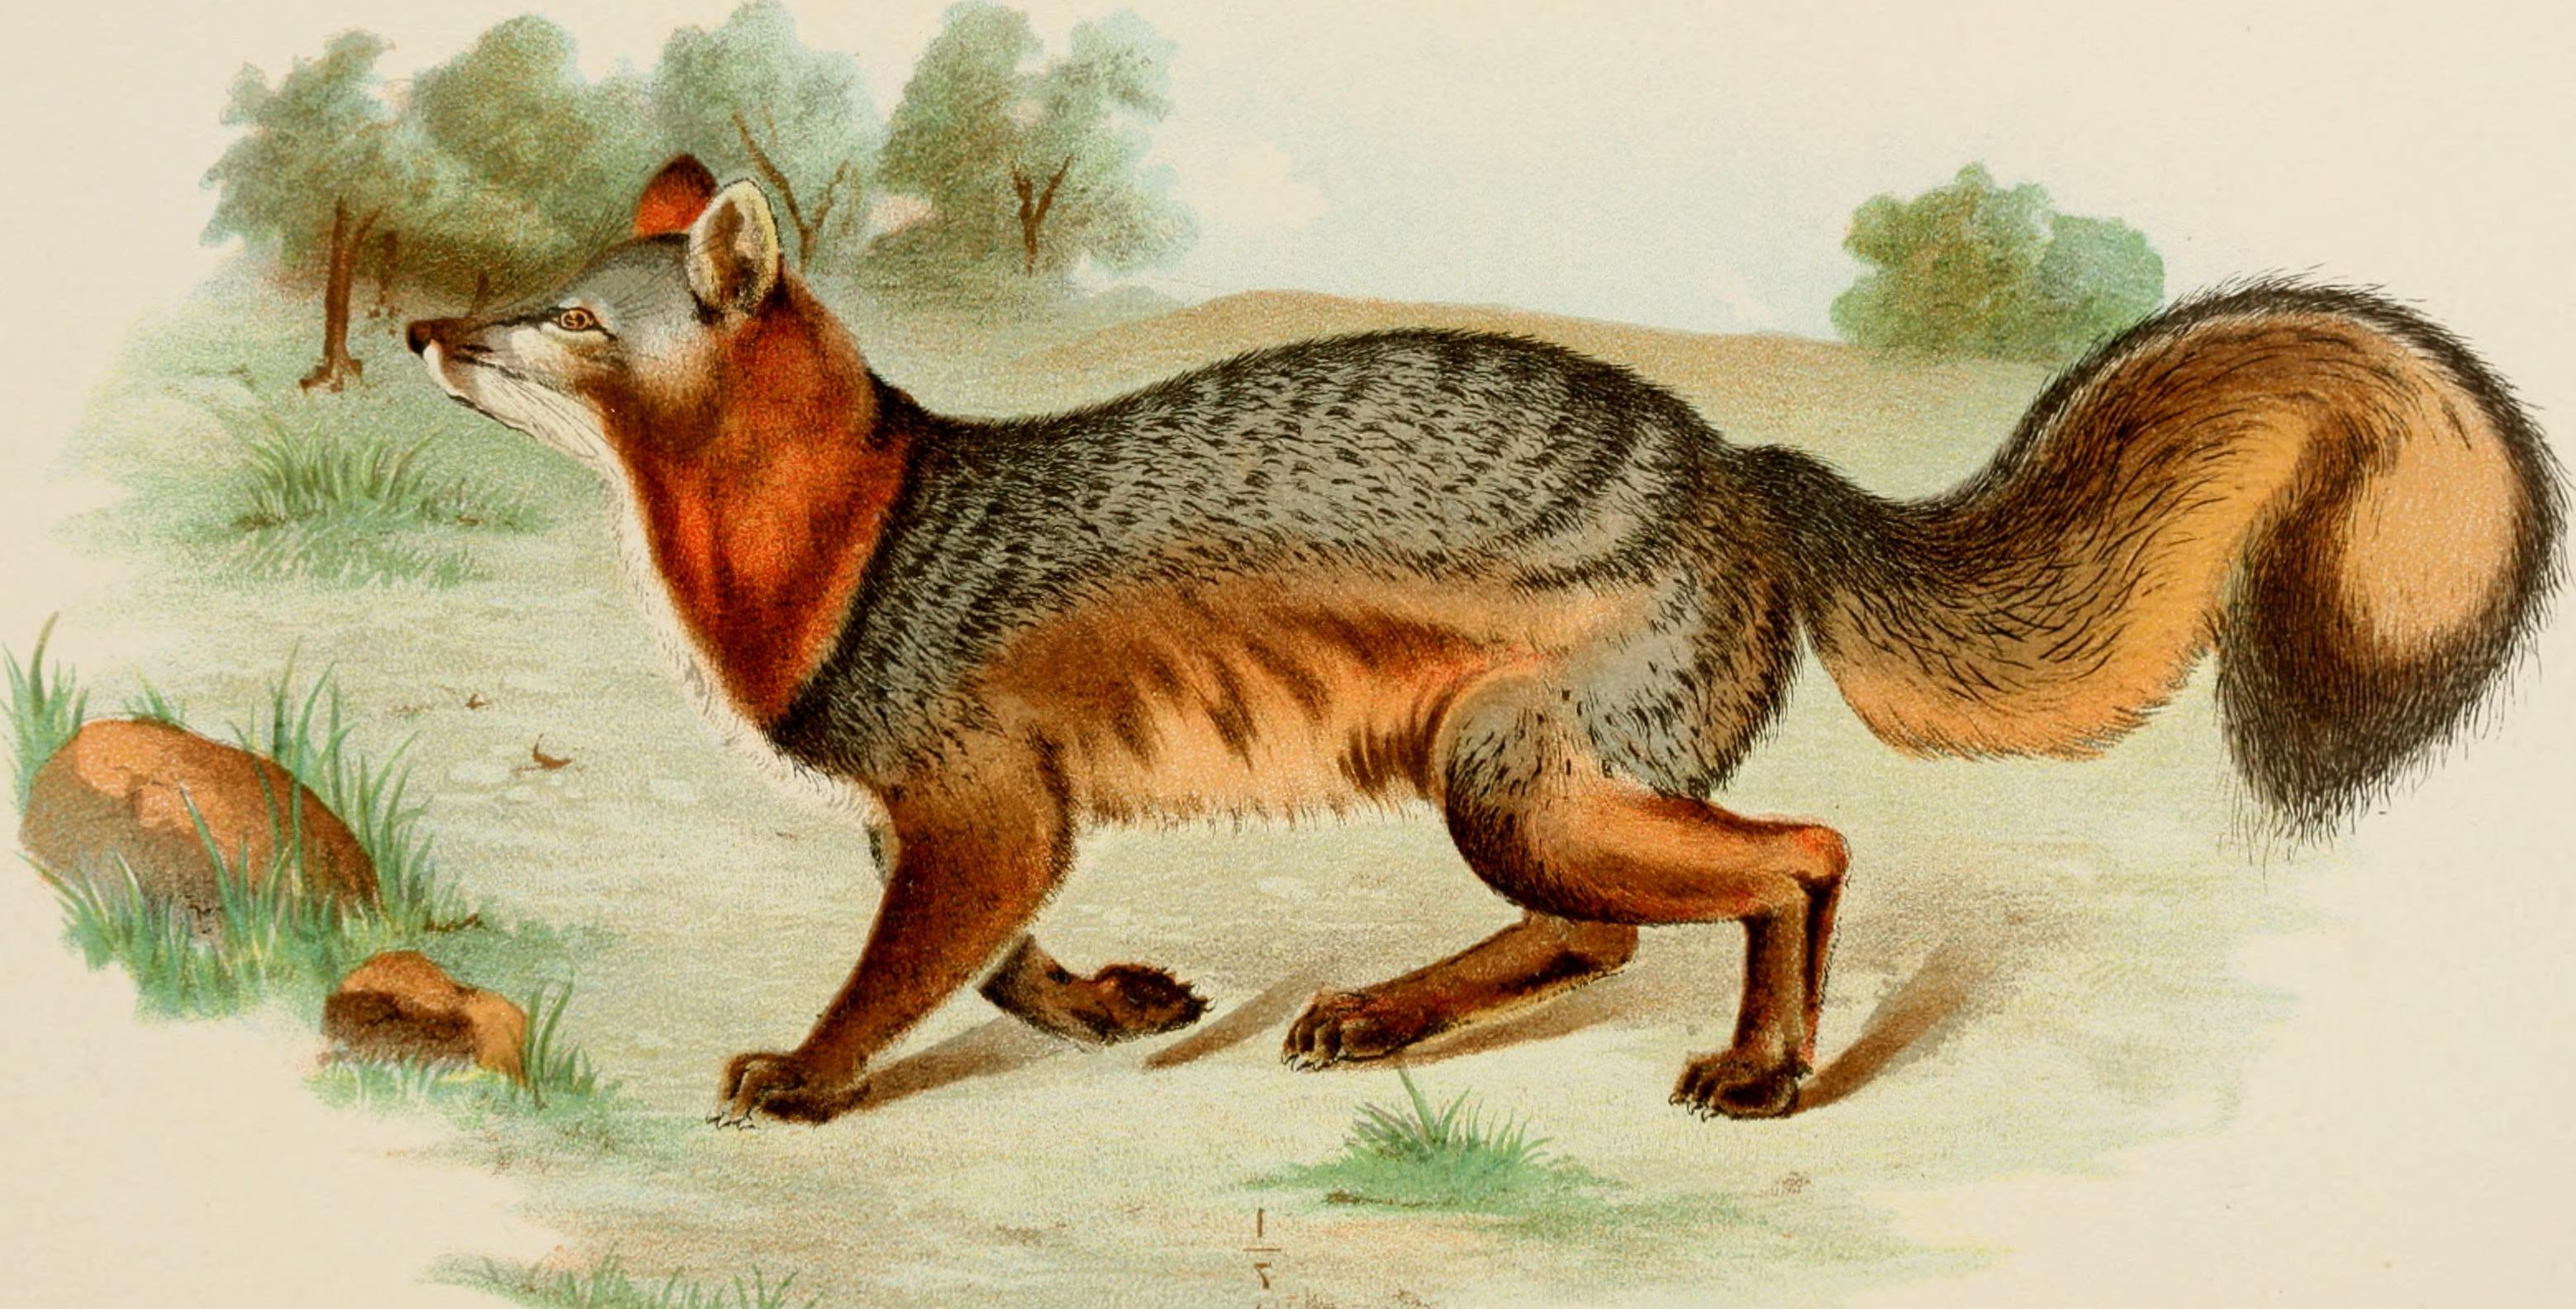
\includegraphics[width =
  \textwidth]{illustration_images/Quant_gen/Grey_fox/14770789583_4db7ec5164_o.jpg}  %https://www.flickr.com/photos/internetarchivebookimages/14770789583/in/photolist-axdicF-ovfa8V-odM3sY-bCrnQ8-ovgYXn-tiQfMQ-odMpu5-x1xCJu-wQ7qT7-wE7kfs-xEZQd1-wK4YSh-ovWx4g-wpDZzF-xjvQ89-tHDjuS-w9Wit5-xEvyhH-xjCbKD-u4q3Qe
\end{center}
\caption{Gray Fox, {\it Urocyon cinereoargenteiis}. \BHLNC{Diseases and enemies of poultry. Pearson and Warren. (1897)}{https://archive.org/stream/diseasesenemieso00pearrich/diseasesenemieso00pearrich\#page/n663/mode/1up}{University of California Libraries}} 
\end{marginfigure}


\begin{question}
\citet{robinson:16} found that the endangered Californian Channel Island fox on San Nicolas had very
low levels of diversity ($\pi =0.000014 \text{bp}^{-1}$) compared to
its close relative the California mainland gray fox ($0.0012\text{bp}^{-1}$). \\
%\bf A How many sites do you expect to differ between two samples
%sequenced over a 100kb region in each of these populations?\\   
{\bf A)} Assuming a mutation rate of $2\times 10^{-8}$ per bp, what
effective population sizes do you estimate for these two populations?
\\
{\bf B)} Why is the effective population size of the Channel Island fox
so low? [Hint: quickly google Channel island foxes to read up on their
history, also to see how ridiculously cute they are.]
\end{question}


\begin{question}
In your own words describe why the coalescent time of a pair of lineages scales linearly with the (effective) population size.
%The long-term $N_e$ estimated from genetic diversity within most human populations is roughly $10,000$, and the generation time of humans is $\sim$30 years. What is the average time, in years, that we have to go back to to find the most recent common ancestor for  a pair of sequences drawn from the same human population?
\end{question}


\paragraph{More details on the pairwise coalescent and the randomness of mutation.}

We've derived the expected number of differences between a pair of sequences and talked about how variable the coalescent time is for a pair of sequences. The mutation process is also very variable; even if two sequences coalesce in the very distant past by chance, they may still be identical in the present if there was no mutation during that time. 

Conditional on the coalescent time $t$, the probability that our pair of alleles are separated by $S_2$ mutations since they last shared a common ancestor is
\begin{equation}
P(S_2 | T_2 = t ) = {2t \choose j} \mu^{j} (1-\mu)^{2t-j}
\end{equation}
i.e. mutations happen in $j$ generations and do not happen in $2t-j$
generations (with ${2t \choose j}$ ways this combination of events can possibly
happen). Assuming that $\mu \ll 1$ and that $2t-j \approx 2t$, then we
can approximate the probability that we have $S_2$ mutations as a
Poisson distribution:
\begin{equation}
P(S_2 | T_2 = t ) = \frac{ (2 \mu t )^{j} e^{-2\mu t}}{j!}
\end{equation}
i.e. a Poisson with mean $2\mu t $. We'll not make much use of this result, but it is very useful in thinking about how to simulate the process of mutation.\\

\section{The coalescent process of a sample of alleles.}

Usually we are not just interested in pairs of alleles, or the
average pairwise diversity. Generally we are interested in the properties of
diversity in samples of a number of alleles drawn from the population.  
Instead of just following a pair of lineages back until they
coalesce, we can follow the history of a sample of alleles back
through the population.

Consider first sampling three alleles at random from the population. The
probability that all three alleles choose exactly the same ancestral allele one
generation back is $\nicefrac{1}{(2N)^2}$. If $N$ is reasonably large, then this
is a very small probability. As such, it is very unlikely that our three alleles
coalesce all at once, and in a moment we'll see that it is safe to ignore such
unlikely events. \\

\begin{figure}
\begin{center}
  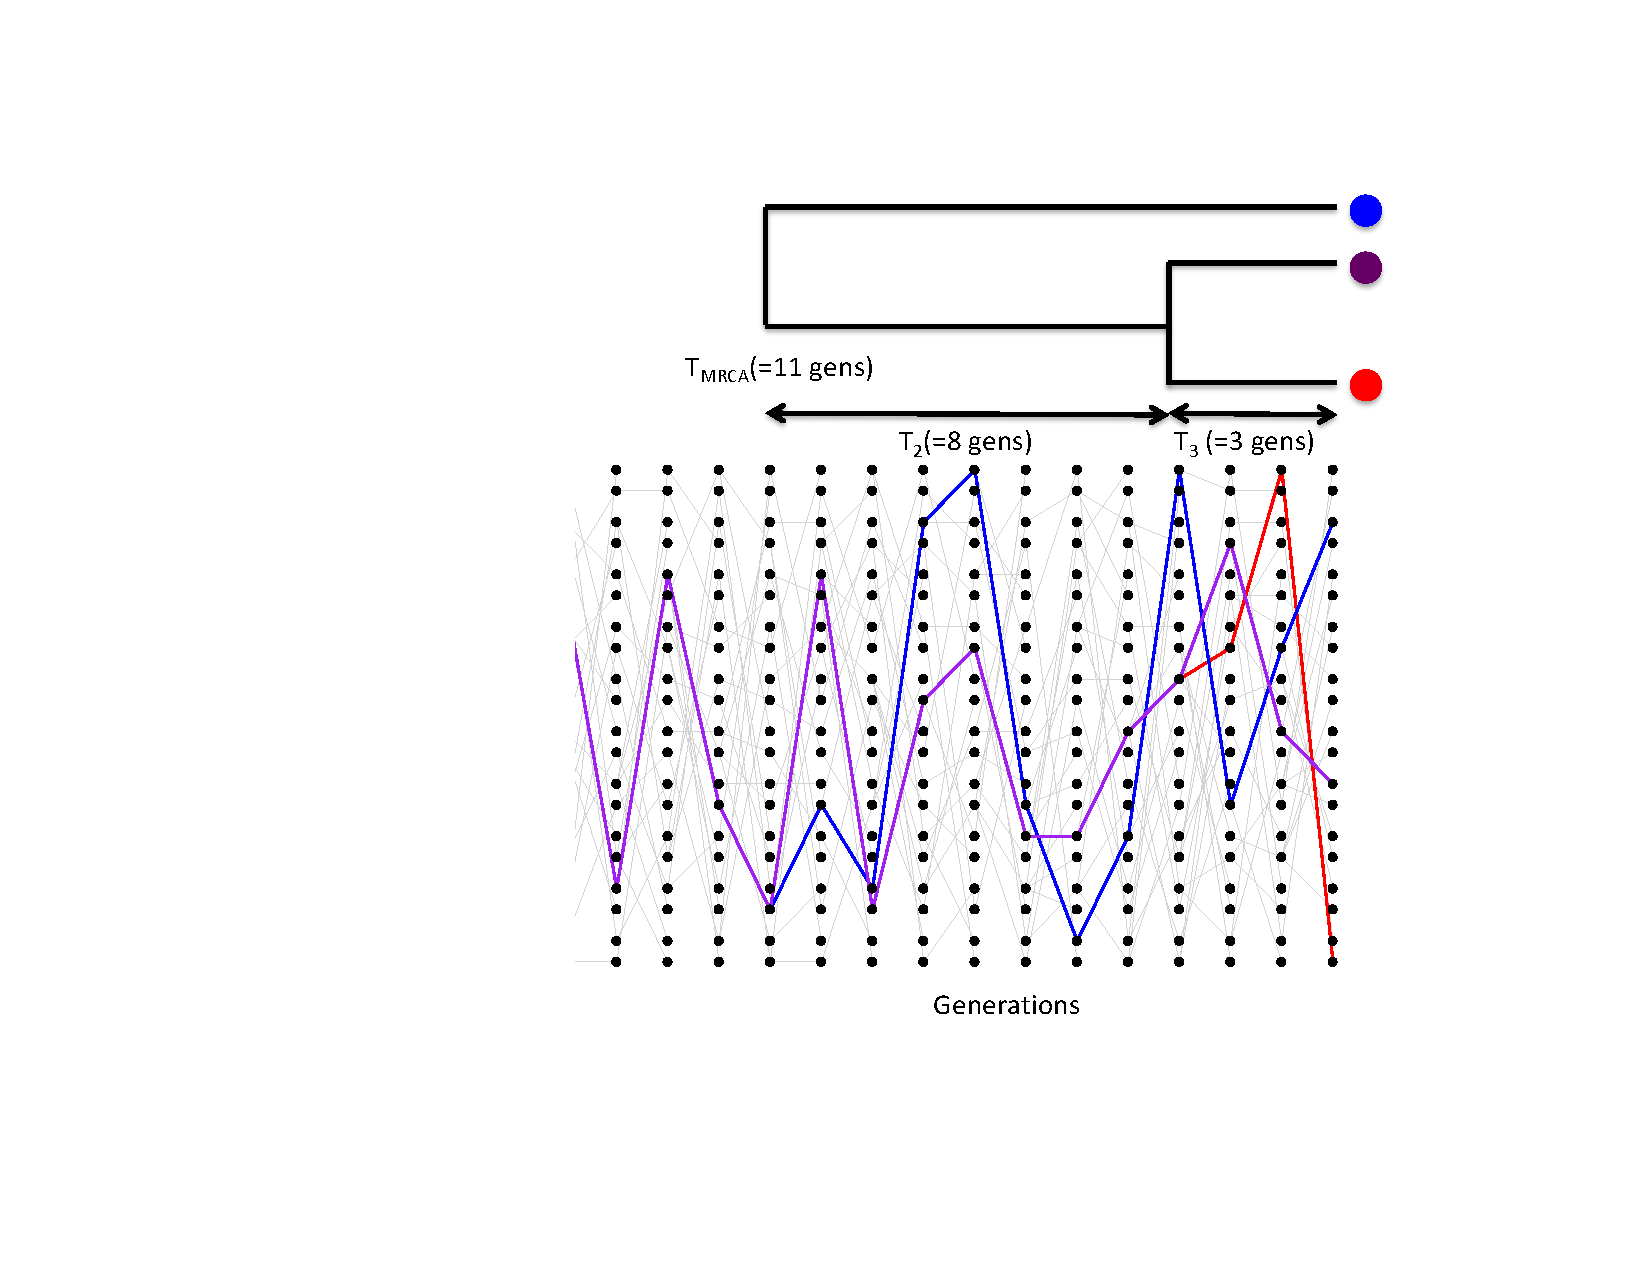
\includegraphics[width = 0.75 \textwidth]{figures/Coalescent/Coal_three_lineages.pdf}
\end{center}
\caption{A simple simulation of the coalescent process for three
  lineages. We track the ancestry of 
  three modern-day alleles, the first pair (blue and purple) coalesce four generations back, after which  
  there are only two independent lineages we are tracking. This pair
  then coalesces twelve generations in the past. Note that different
  random realizations of this process will differ from each other a lot. The $T_{MRCA}$ is $T_3+T_2$. The total time in the tree is $T_{tot}=3T_3 + 2T_2= 25$ generations. \gitcode{https://github.com/cooplab/popgen-notes/blob/master/Rcode/track_alleles.R} } \label{fig:Coalescent_simulation_3}
\end{figure}

The probability that a specific pair of alleles find a common ancestor in the
preceding generation is still $\nicefrac{1}{(2N)}$. There are three possible pairs of
alleles, so the probability that no pair finds a common ancestor in the preceding generation is
\begin{equation}
\left(1-\frac{1}{2N} \right)^3 \approx \left( 1- \frac{3}{2N} \right)
\end{equation}
In making this approximation we are multiplying out the right hand-side
and ignoring terms of $1/N^2$ and higher. See
Figure \ref{fig:Coalescent_simulation_3} for a random realization of this process. \\

More generally, when we sample $i$ alleles there are ${i \choose 2}$
pairs,\sidenote{said as ``i choose 2''}  i.e. $i(i-1)/2$ pairs. Thus, the probability that no pair
of alleles in a sample of size $i$ coalesces in the preceding generation is
\begin{equation}
\left(1-\frac{1}{(2N)} \right)^{{i \choose
 2}} \approx \left( 1- \frac{{i \choose
 2}}{2N}\right)
\end{equation}
while the probability any pair coalesces is $\approx \nicefrac{2N}{{i \choose
 2}}$.\\

We can ignore the possibility that more than pairs of alleles (e.g. tripletons)
simultaneously coalesce at once as terms of $\nicefrac{1}{N^2}$ and higher
can be ignored as they are vanishingly rare. Obviously in reasonable
sample sizes there are many more triples (${i \choose 3}$) and higher order
combinations than there are pairs (${i \choose 2}$), but if $i \ll N$ then we are safe to
ignore these terms.


When there are $i$ alleles, the probability that we wait until the
$t+1$ generation before
any pair of alleles coalesces is
\begin{equation}
P(T_i =t+1) = \frac{{i \choose
 2}}{2N}\left( 1- \frac{{i \choose
 2}}{2N}\right)^{t} \label{eqn:T_i}
\end{equation}
Thus the waiting time to the first coalescent event while there are $i$ lineages is a geometrically distributed random variable with probability of success $\nicefrac{{i \choose 2}}{2N}$, which we denote by
\begin{equation}
T_i \sim \text{Geo}
\left(  \nicefrac{{i \choose
      2}}{2N} \right).
\end{equation}
The mean waiting time till any of pair within our
 sample coalesces is 
\begin{equation}
\E( T_i) = \frac{2N}{{i \choose  2}}  \label{eqn:E_T_i}
\end{equation}
\marginnote{
To see the continuous time  version of this, note that \eqref{eqn:T_i} is
\begin{equation} 
\approx  \frac{{i \choose
 2}}{2N} \exp \left( - \frac{{i \choose
 2}}{2N} t \right)
\end{equation}
The waiting time $T_i$ to the first coalescent event in a sample
of $i$ alleles is thus exponentially distributed with rate $\nicefrac{{i \choose
 2}}{2N}$, i.e. $T_i \sim \text{Exp}\left(\nicefrac{{i \choose
 2}}{2N} \right)$. }
After a pair of alleles first finds a common ancestral allele some
number of generations back in the past, we only have to keep
track of that common ancestral allele for the pair when looking further into the past. Thus when a pair
of alleles in our sample of $i$ alleles coalesces, we then switch to
having to follow $i-1$ alleles back in time. Then when a pair of these $i-1$
alleles coalesce, we then only have to follow $i-2$ alleles back. This
process continues until we coalesce back to a sample of two, and from
there to a single most recent common ancestor (MRCA).\\


\paragraph{Simulating a coalescent genealogy}
To simulate a coalescent genealogy at a locus for a sample of $n$ alleles we therefore simply follow the following
algorithm:
\begin{enumerate}
\item Set $i=n$.
\item Simulate a random variable to be the time $T_i$ to the next coalescent event from $T_i \sim
  \text{Exp}\left(\nicefrac{{i \choose
 2}}{2N} \right)$
\item Choose a pair of alleles to coalesce at random from all possible
 pairs.
\item Set $i=i-1$
\item Continue looping steps 1-3 until $i=1$, i.e. the most recent
 common ancestor of the sample is found.
\end{enumerate}
By following this algorithm we are generating realizations of the
genealogy of our sample. \\



\subsection{Expected properties of coalescent genealogies and
  mutations.} 

\begin{figure}
\begin{center}
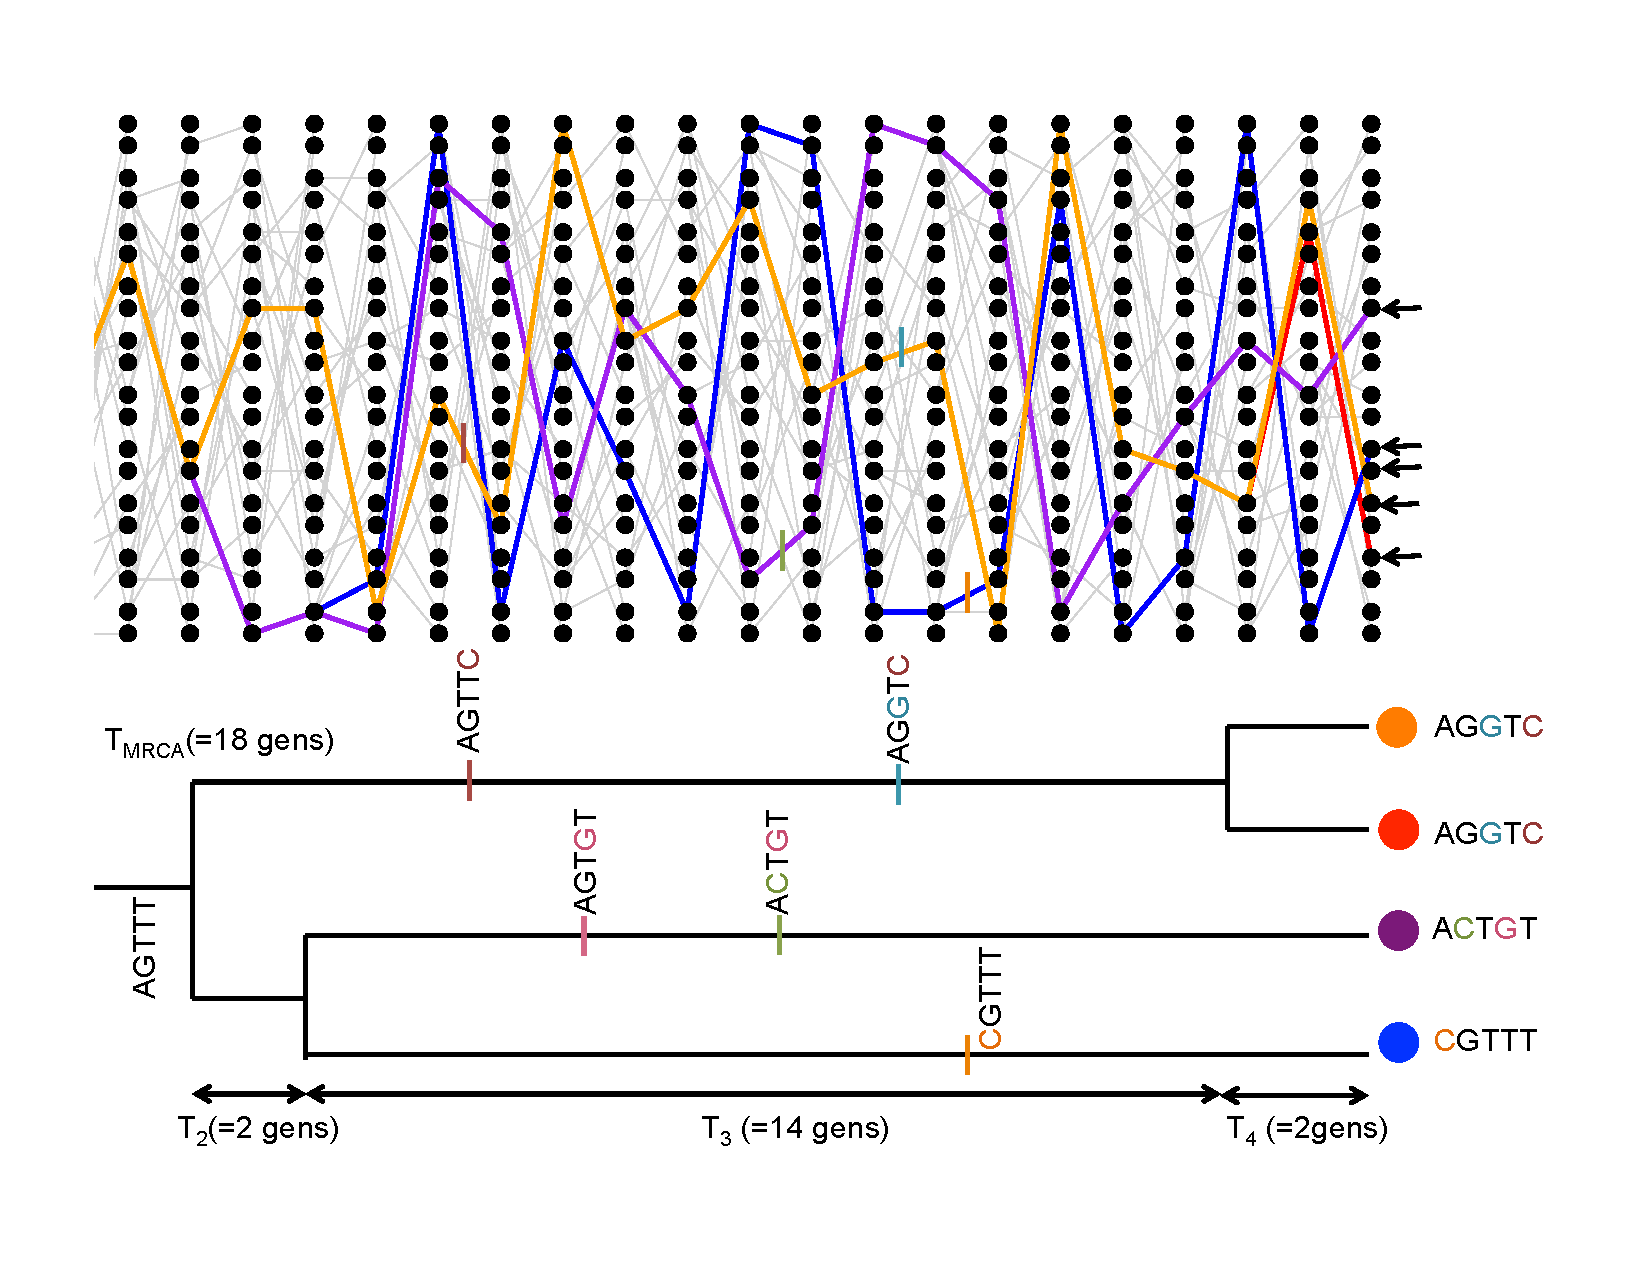
\includegraphics[width= \textwidth]{figures/Coalescent/Coal_w_muts.pdf}
\end{center}
\caption{A simple coalescent tree from a single coalescent simulation, tracing the genealogy of 4 alleles with mutational changes marked with dashes showing transitions away from the MRCA sequence (AGTTT) . The $T_{MRCA}$ is $T_4+T_3+T_2$. The total time in the tree is $T_{tot}=4 T_4+3T_3 + 2T_2= 54$ generations. \gitcode{https://github.com/cooplab/popgen-notes/blob/master/Rcode/track_alleles.R}  } \label{fig:Coal_w_muts}
\end{figure}


\paragraph{The expected time to the most recent common ancestor.}
We will first consider the time to the most recent common ancestor of
the entire sample ($T_{MRCA}$). This is
\begin{equation}
T_{MRCA} = \sum_{i=n}^2 T_i
\end{equation}
generations back, where we are summing from $i=n$ alleles counting backwards to $i=2$ alleles (see Figure \ref{fig:Coal_w_muts} for example). As our coalescent times for different $i$ are independent, the expected time to the most recent common ancestor
is
\begin{equation}
\E(T_{MRCA}) = \sum_{i=n}^2 \E(T_i) = \sum_{i=n}^2  2N/{i \choose
 2}
\end{equation}
Using the fact that $\frac{1}{i(i-1)}=\frac{1}{i-1} - \frac{1}{i}$ and a bit of
rearrangement, we can rewrite this as
\begin{equation} 
\E(T_{MRCA}) = 4N\left(1- \frac{1}{n} \right) \label{TMRCA_neutral}
\end{equation}
So the average $T_{MRCA}$ scales linearly with population
size $N$. Interestingly, as we move to larger and larger samples (i.e. $n \gg 1$), the average
time to the most recent common ancestor converges on $4N$. What's
happening here is that in large samples our lineages typically coalesce rapidly
at the start and very soon coalesce down to a much smaller number of
lineages.   \\

\begin{question}
Assume an autosomal effective population of 10,000 individuals (roughly the long-term human estimate) and a generation time of 30 years. What is the expected time to the most recent common ancestor of a sample of 20 people? What is this time for a sample of 500 people?  
\end{question}
\paragraph{The expected total time in a genealogy and the number of
  segregating sites.}

Mutations fall on specific lineages of the coalescent genealogy and are transmitted to all descendants of their lineage. Furthermore, under the infinitely-many-sites assumption, each mutation creates a new segregating site. The mutation process is a
\emph{Poisson process}, and the longer a particular lineage, i.e. the more generations of meioses it represents, the more
mutations that can accumulate on it. The total number of segregating sites in
a sample is thus a function of the \emph{total} amount of time in the
genealogy of the sample, or the sum of all the branch lengths on the genealogical tree,
$T_{tot}$. Our total amount of time in the genealogy is

\begin{equation}
T_{tot} = \sum_{i=n}^2 iT_i
\end{equation}
as when there are $i$ lineages, each contributes a time $T_i$ to the total time (see Figure \ref{fig:Coal_w_muts} for an example). Taking the expectation of the total time in the genealogy,
\begin{equation}
\E(T_{tot}) = \sum_{i=n}^2 i \frac{2N}{{i \choose
 2} } = \sum_{i=n}^2 \frac{4N}{i -1} =\sum_{i=n-1}^1 \frac{4N}{i} \label{eqn:E_T_tot}
\end{equation}
we see that our expected total amount of time in the genealogy scales linearly
with our population size $N$. Our expected total amount of time is also
increasing with sample size $n$, but is doing so very slowly. %To see this
%more carefully, we can see that for large $n$
%\begin{equation}
%\E(T_{tot}) = \sum_{i=n-1}^1 \frac{4N}{i} 
%\end{equation}
\marginnote{To get a better sense of how $T_{tot}$ grows with the sample size, we
  can approximate the sum \ref{eqn:E_T_tot} by an integral, which will work for large $n$. The result is  $\int_1^{n-1} \frac{4N}{i} di
= 4N \log(n-1)$. }
This again follows
from the fact that in large samples, the initial coalescence usually
happens very rapidly, so that extra samples add little to the total
amount of time in the genealogical tree. \\

We saw above that the number of mutational differences between a pair
of alleles that coalescence $T_2$ generations ago was Poisson with a
mean of $2 \mu T_2$, where $2T_{2}$ is the total branch length in this simple 2-sample genealogical tree. A mutation that occurs on any branch of our
genealogy will cause a segregating polymorphism in the sample
(meeting our infinitely-many-sites assumption). Thus, if the total time
in the genealogy is $T_{tot}$, there are $T_{tot}$
generations for mutations. So the total number of mutations
segregating in our sample ($S$) is Poisson with mean $\mu T_{tot}$. Thus the
expected number of segregating  sites in a sample of size $n$ is
\begin{equation}
\E(S) = \mu \E(T_{tot}) = \sum_{i=n-1}^1 \frac{4N\mu }{i} = \theta
\sum_{i=n-1}^1 \frac{1}{i}
\end{equation}
Note that this is growing with the sample size $n$, albeit very slowly (roughly at the rate of the $\log$ of the sample size). 
We can use this formula to derive another estimate of the population scaled mutation rate $\theta$, by setting our observed number of segregating sites in a sample ($S$) equal to this expectation. We'll call this estimator $\widehat{\theta}_W$:
\begin{equation}
\widehat{\theta}_W =\frac{ S}{\sum_{i=n-1}^1 \nicefrac{1}{i}}   \label{watterson_theta}
\end{equation}
This estimator of $\theta$ was devised by \citet{watterson:75}, hence the $W$.


\paragraph{The neutral site-frequency spectrum.}

We can use our coalescent process to find the expected number of
derived alleles present $i$ times out of a sample size $n$, e.g. how many singletons ($i = 1$) do we
expect to find in our sample? For example, in Figure \ref{fig:Coal_w_muts} in our sample of four sequences, there are 3 singletons and 2 doubletons. The number of sites with these different allele frequencies depends on the lengths of specific genealogical branches. A mutation that falls on a branch with $i$ descendants will create a derived allele with frequency $i$. For example, in our example tree  in Figure \ref{fig:Coal_w_muts}, the total number of generations where a mutation could arise and be a doubleton is $T_3+2T_2$, the total length of the branch ancestral to just the orange and red allele $(T_3+T_2)$ plus the branch ancestral to just the blue and purple allele $(T_2)$. 

\begin{marginfigure}[-4cm]
\begin{center}
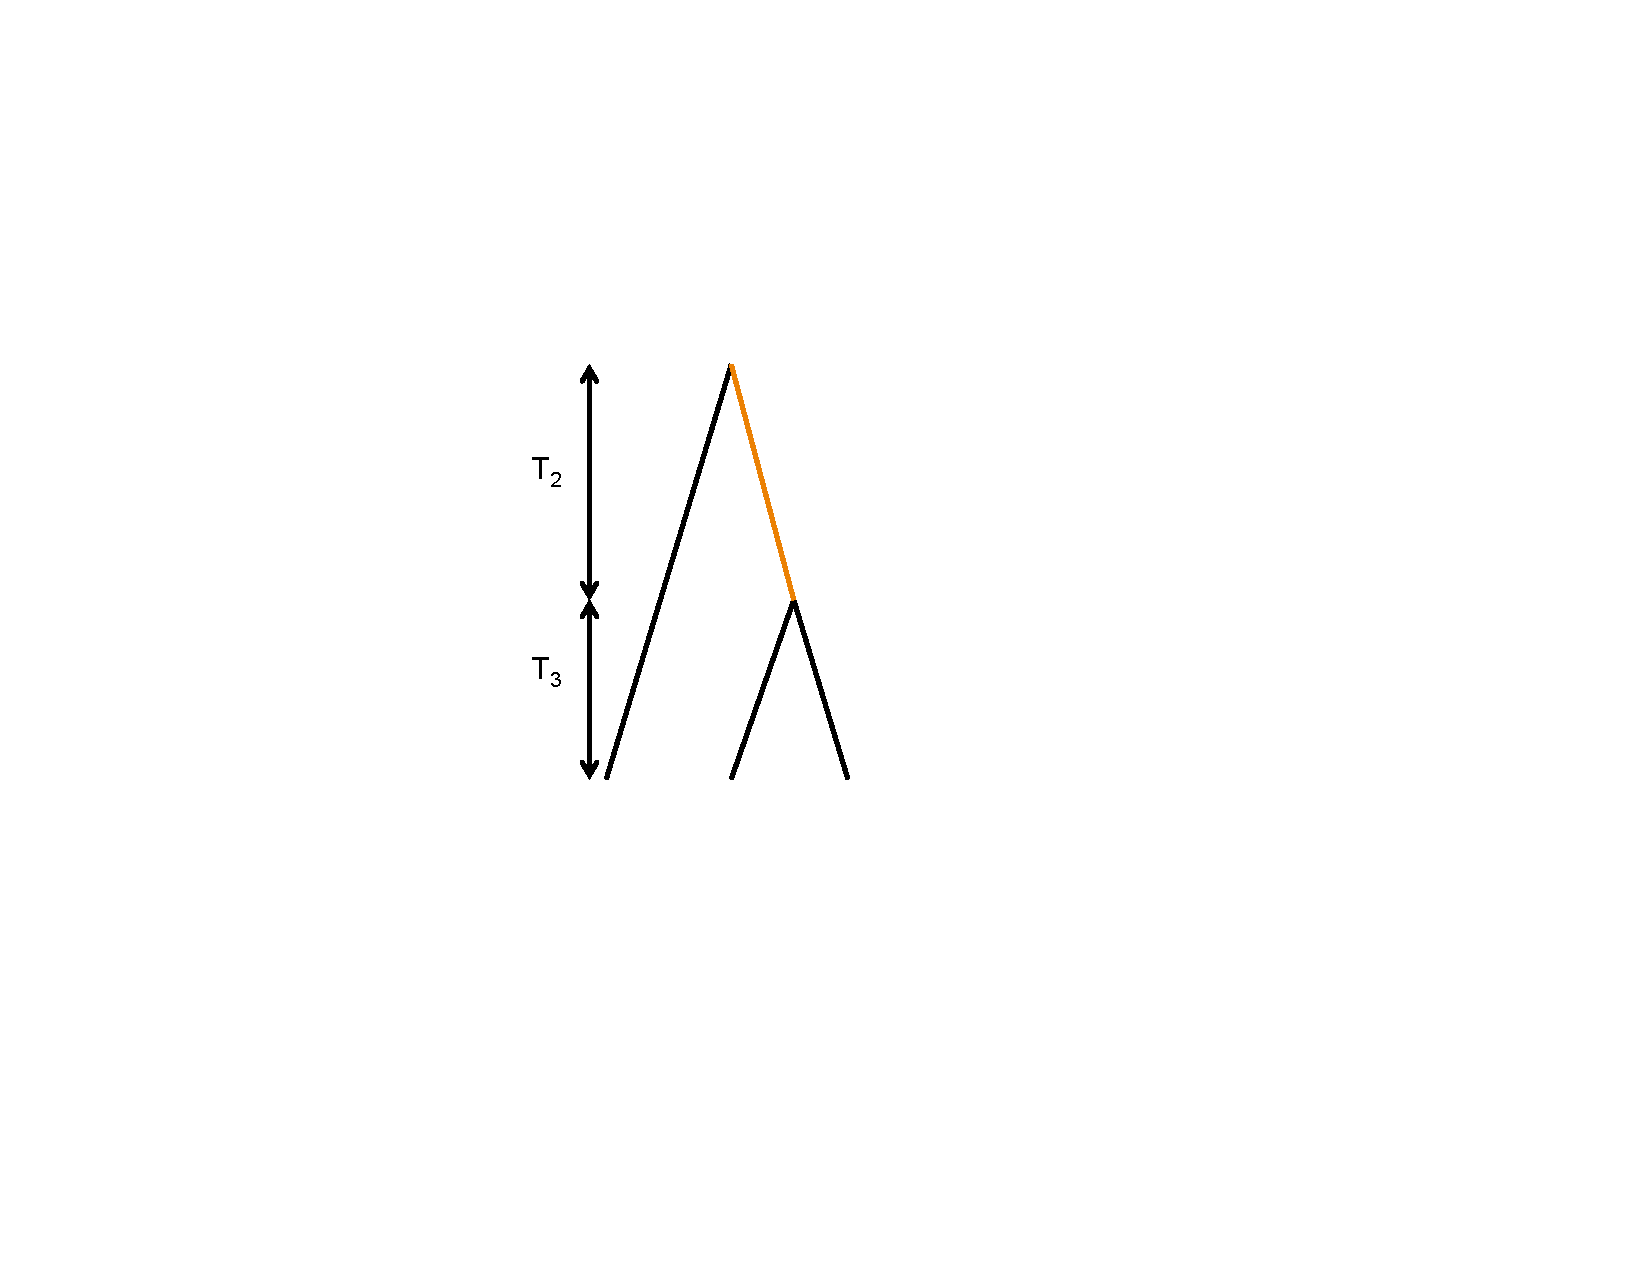
\includegraphics[width= \textwidth]{figures/Genetic_drift/freq_spec_tree.pdf}
\end{center}
\caption{A tree for three samples; note that this is the only possible
tree shape (treating the tips as unlabeled, i.e.  I don't care which pair of sequences carry a doubleton, just that any two sequences carry a derived allele).} \label{fig:freq_coal}
\end{marginfigure}

To see how we could go about working this out, lets start by considering the simple coalescent tree, shown in Figure \ref{fig:freq_coal}, for sample of $3$ alleles drawn from a population. Mutations that fall on the
branches coloured in black will be derived singletons, while mutations that
fall along the orange branch will be doubletons in the sample. The
total number of generations where a singleton mutation could arise is
$3 T_3 + T_2$. Note that we only count the time where there are two
lineages $(T_{2})$ once. So our expected number of singletons, using eqn \eqref{eqn:E_T_i}, is 
\begin{equation}
\E(S_i) = \mu \left( 3\E(T_3) +  \E(T_2) \right) = \mu \left( 3
  \frac{2N}{3}+ 2N \right) = \theta
\end{equation}
By similar logic, the time where doubletons could arise is
$T_2$ and our expected number of doubletons is $\E(S_i)
=\theta/2$. Thus, there are on average half as many doubletons as singletons. 

Extending this logic to larger samples might be doable, but is tedious (I mean really tedious: for 10 alleles there are thousands of possible tree shapes and the task quickly gets impossible even computationally). A nice, relatively simple proof of the neutral site frequency spectrum is given by
\citeauthor{Hudson:15}, but we won't give this here. The general form is: 
\begin{equation}
\E(S_i) = \frac{\theta }{i}   \label{eqn:neutral_freq_spec}
\end{equation}
i.e. there are twice as many singletons as doubletons, three times as many
singletons as tripletons, and so on. The other thing that will be
helpful for us to know is that neutral alleles at intermediate frequency tend to be old, and those that are rare in the sample are young. We expect to see a lot more rare alleles in our sample than common alleles. 

\begin{question}
There are two possible tree shapes that could relate four
samples. Draw both of them and separately colour (or otherwise mark) the branches by where singletons, doubletons, and tripleton derived alleles could arise. 
%{\bf A)} 
%{\bf B)} Can you work out the expected number of each allele count? [{\bf OPTIONAL}] \erin{change for different tree question}
\end{question}

We can also ask the probability of observing a derived allele segregating at frequency $i/n$ given that the site is polymorphic in our sample of size $n$ (i.e. given that $0<i<n$ ). We can obtain this probability by dividing the expected number of sites segregating for an allele at frequency $i$ by the expected number segregating at all of the possible allele frequencies for polymorphisms in our sample 
\begin{eqnarray}
P(i |0<i<n) &=\frac{\E(S_i)}{\sum_{j=1}^{n-1} \E(S_j)} = \frac{\nicefrac{1}{i}}{\sum_{j=1}^{n-1} \nicefrac{1}{j}}.
\end{eqnarray}
We can interpret this probability as the fraction of polymorphic sites we expect to find at a frequency $i/n$. 

\paragraph{tests based on the site frequency spectrum}
Population geneticists have proposed a variety of ways to test whether an observed site frequency spectrum conforms to its
neutral, constant-population expectations. These tests are
useful for detecting population size changes using data across many loci, or
for detecting the signal of selection at individual loci. One of
the first tests was proposed by \citeauthor{tajima:89}, and is called
Tajima's $D$. Tajima's $D$ is
\begin{equation}
  D = \frac{\theta_{\pi}-\theta_{W}}{C} \label{eqn_Tajimas_D}
\end{equation}
where the numerator is the difference between the estimate of
$\theta$ based on pairwise differences and that based on segregating
sites. As these two estimators both have expectation $\theta$ under
the neutral, constant-population model, the expectation of $D$ is zero. The denominator $C$ is a positive constant; it's the square-root of an estimatorof the variance of this difference under the constant population size, neutral model. This constant was chosen for $D$ to have mean zero and variance $1$ under the null model, so we can test for  departures from this simple null model.\\

An excess of rare alleles compared to the constant-population, neutral
model will result in a negative Tajima's $D$, because each
additional rare allele increases the number of segregating sites by
$1$, but only has a small effect on the number of pairwise differences between samples. 
In contrast, a positive Tajima's $D$ reflects an excess of intermediate frequency alleles relative to the constant-population, neutral expectation. Alleles at intermediate-frequency increase pairwise diversity
more per segregating site than typical, thus increasing $\theta_{\pi}$ more than $\theta_{W}$.

\subsection{Demography and the coalescent}

\begin{marginfigure}
\begin{center}
  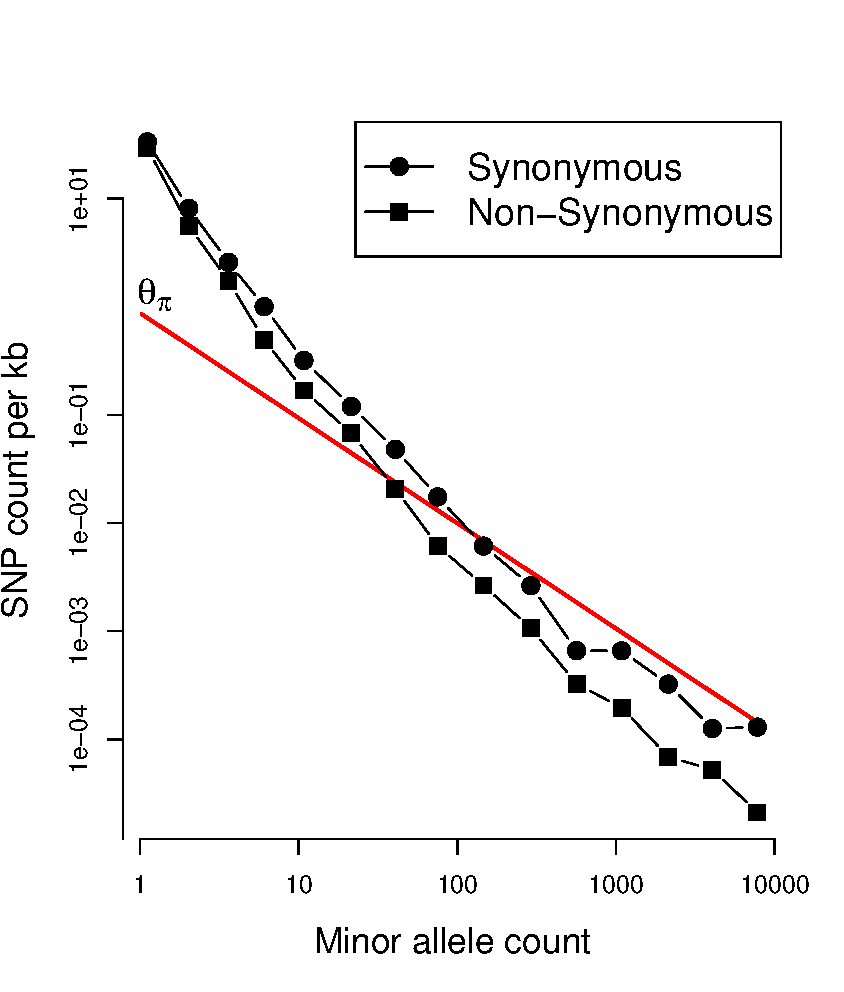
\includegraphics[width = \textwidth]{Journal_figs/genetic_drift/human_pop_growth/Nelson_pop_growth.pdf}
\end{center}
\caption{Data from 202 genes from 14002 people of European ancestry (28004 alleles). Note
  the double log-scale. Redrawn from \citeauthor{nelson:12}. The red
  line gives the neutral, constant population size estimate of the site frequency spectrum, our equation \eqref{eqn:neutral_freq_spec}, using a  $\theta$ estimated from $\pi$. Note how the non-synonymous changes are even more skewed towards rare alleles, that's likely due to selection against non-synonymous alleles acting to push them towards rare frequency. \gitcode{https://github.com/cooplab/popgen-notes/blob/master/Journal_figs/genetic_drift/human_pop_growth/Nelson_pop_growth.R} } \label{fig:Human_growth}
\end{marginfigure}
We've already seen how changes in population size can change the rate
at which heterozygosity is lost from the population (see the
discussion around eqn. \eqref{eqn:var_pop_coal}). If the population
size in generation $i$ is $N_i$, the probability that a pair of
lineages coalesce is $\nicefrac{1}{2N_i}$; this conforms to our
intuition that if the population size is small, the rate at which
pairs of lineages find their common ancestor is faster. We can potentially accommodate rapid random fluctuations in population size by simply using the effective population size $N_e$ in place of $N$. However,
longer term more systematic changes in population size will distort
the coalescent genealogies, and hence patterns of diversity, in more
systematic ways. 

We can see how demography potentially distorts the observed frequency spectrum away from the neutral expectation in a very large sample of humans shown in Figure \ref{fig:Human_growth}. For
comparison, the neutral frequency spectrum, eqn
\eqref{eqn:neutral_freq_spec}, is shown as a red line. There are
  vastly more rare alleles than expected under our neutral, constant-population-size model, but the neutral prediction and reality agree somewhat more for alleles that are more common.  

\begin{figure*}
\begin{center}
  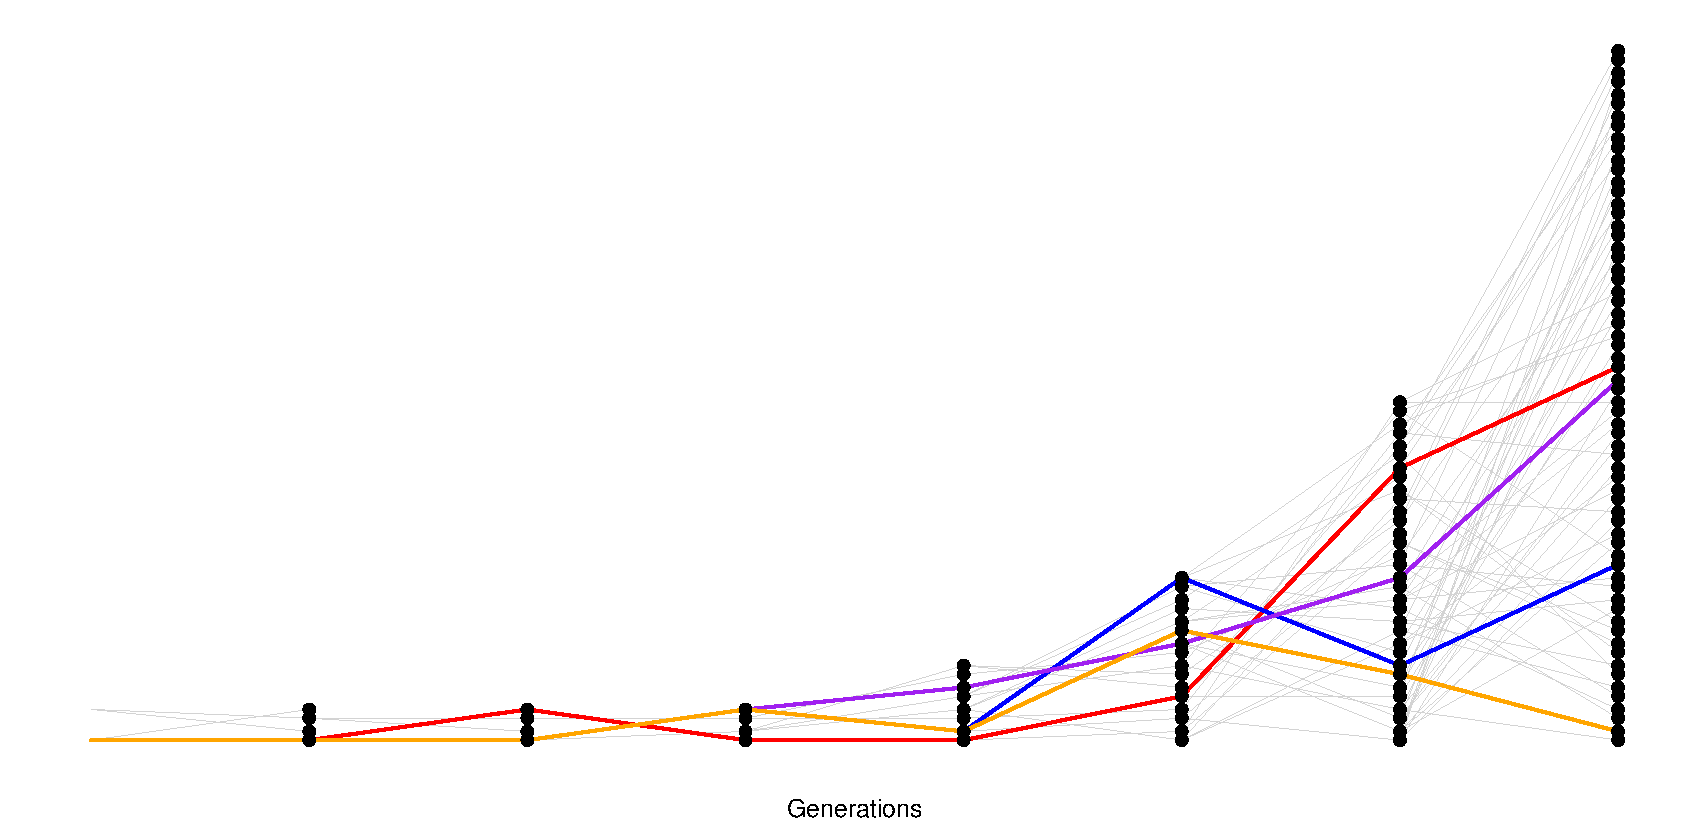
\includegraphics[width = \textwidth]{figures/Genetic_drift/Demography/Growth_genealogy.pdf}
\end{center}
\caption{A realization of the coalescent process in a growing population. The population underwent a period of doubling every generation. The initial population size of just two individuals, maintained for a number of generations, is obviously highly unrealistic but serves our purpose. \gitcode{https://github.com/cooplab/popgen-notes/blob/master/Rcode/track_alleles.R}  } \label{fig:Genealogy_growth}
\end{figure*}

Why is this? Well, these patterns are likely the result of the very recent
explosive growth in human populations. If the population has grown rapidly, then the pairwise-coalescent rate in the past may be much higher than the coalescent rate closer to the present. (see Figure \ref{fig:Genealogy_growth}). 

One consequence of a recent population expansion is that there is much less genetic diversity in the population than you'd predict using the census
population size. Humans are one example of this effect; there are $7$ billion
of us alive today, but this is due to very rapid population growth
over the past thousand to tens of thousands of years. Our level of
genetic diversity is very much lower than you'd predict given our
census size, reflecting our much smaller ancestral population. A second consequence of recent population expansion is that the deeper coalescent branches are much more squished together in time, compared to those in a constant population.  Mutations on deeper branches are the source of alleles at more intermediate frequencies, and so there are even fewer intermediate-frequency alleles
in growing populations. That's why there are so many rare alleles,
especially singletons, in this large sample of Europeans. 


Another common demographic scenario is a population bottleneck. In a bottleneck, the population size crashes dramatically, and subsequently
recovers. For example, our population may have had size $N_{\textrm{Big}}$
and crashed down to $N_{\textrm{Small}}$. One example of a
bottleneck is shown in Figure \ref{fig:Genealogy_crash}. 
\begin{figure*}
\begin{center}
  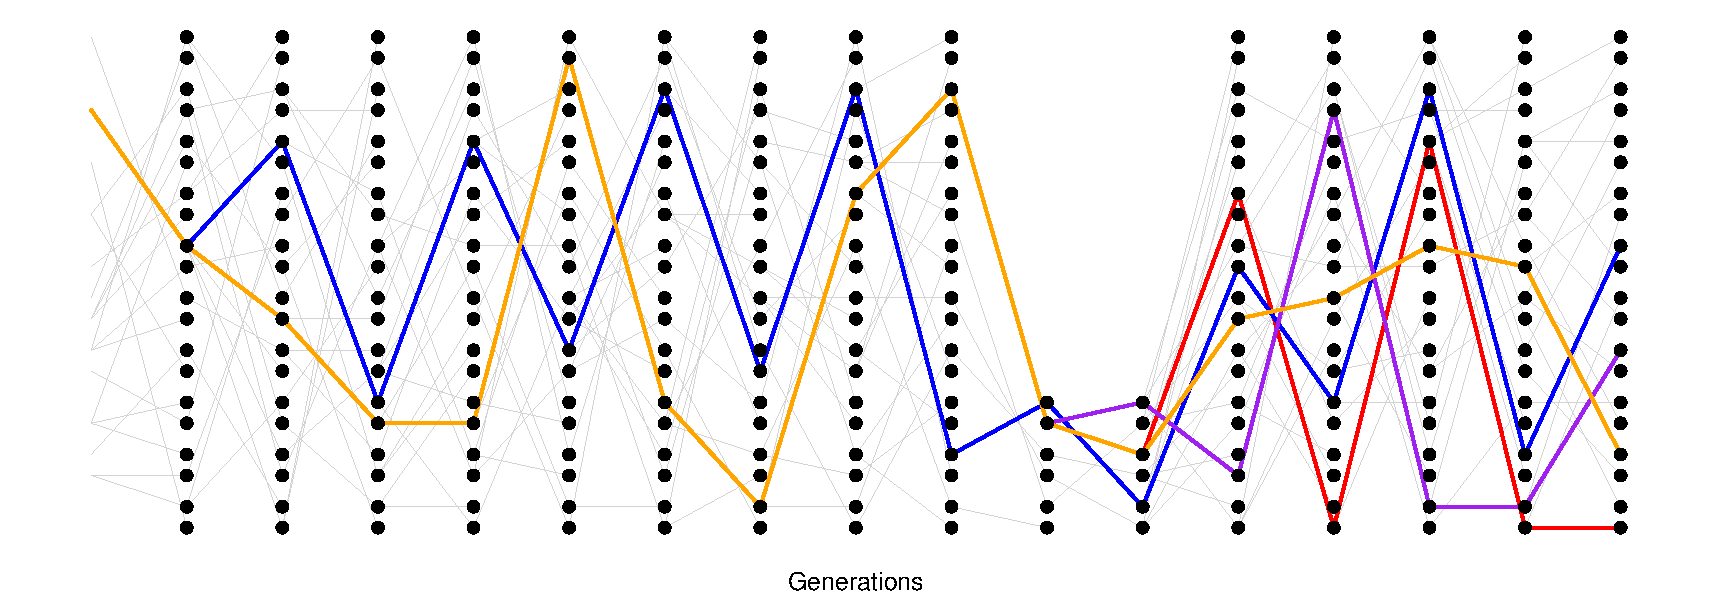
\includegraphics[width = \textwidth]{figures/Genetic_drift/Demography/Crash_genealogy.pdf}
\end{center}
\caption{A realization of the coalescent process in a bottlenecked population. Our population under went a bottleneck eight generations in the past. \gitcode{https://github.com/cooplab/popgen-notes/blob/master/Rcode/track_alleles.R} } \label{fig:Genealogy_crash}
\end{figure*}
Looking at a sample of lineages drawn from the population today, if
the bottleneck was somewhat recent ($\ll N_{\textrm{Big}}$ generations
in the past) many of our lineages will not have coalesced before reaching
the bottleneck, moving backward in time. But during the bottleneck our
lineages coalesce at a much higher rate, such that many of our
lineages will coalesce if the bottleneck lasts long enough
($\sim N_{\textrm{Small}}$ generations). If the bottleneck is very
strong, then all of our lineages will coalesce during the bottleneck, and the resulting site frequency spectrum may
look very much like our population growth model (i.e. an excess of rare
alleles). However, if some pairs of lineages escape coalescing during
the bottleneck, they will coalesce much more deeply in time (e.g. the
blue and orange ancestral lineages in
\ref{fig:Genealogy_crash}). 
\begin{figure}
\begin{center}
  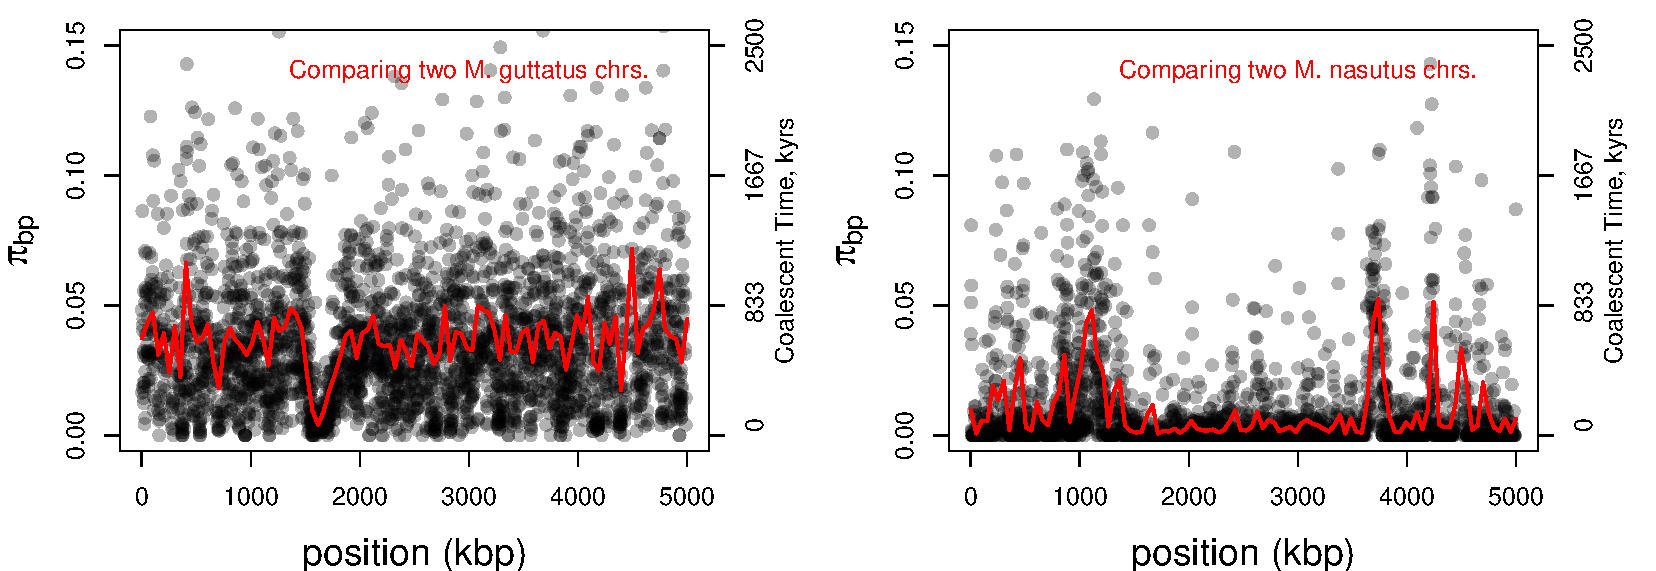
\includegraphics[width = \textwidth]{figures/Genetic_drift/Demography/Mimulus_coalescent_times.pdf}
\end{center}
\caption[][-2cm]{Diversity along the Mimulus genome. Black dots give $\pi$ in 1kb windows between chromosomes sampled from two individuals, the red line is a
  moving average (data from  \citeauthor{brandvain:14}). Pairwise coalescent times ($t$) estimated assuming $t= \nicefrac{\pi}{2 \mu} $ using $\mu_{BP}=10^{-9}$. \gitcode{https://github.com/cooplab/popgen-notes/blob/master/Rcode/Mimulus_coalescent_times.R} } \label{fig:Mimulus_bottleneck}
\end{figure}
\begin{marginfigure}[2cm]
\begin{center}
  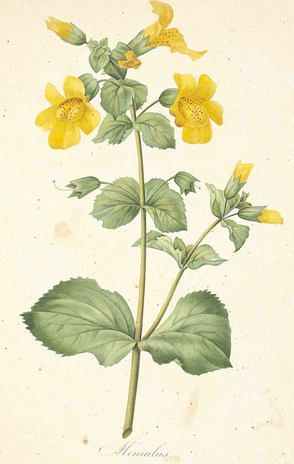
\includegraphics[width = 0.75 \textwidth]{illustration_images/Genetic_drift/Mimulus/Mimulus.png}
\end{center}
\caption{Yellow Monkeyflower {\it M. guttatus}. \newline \noindent \tiny{ Choix des plus belles fleurs et des plus beaux fruits. Pierre-Joseph
  Redout\'e. (1833). Contributed to \href{https://www.flickr.com/photos/swallowtailgardenseeds/14479197839/in/photolist-o4tF54-od9My9-odbSn4-r7eVtm-qrR4xf-x4XVdi-owo7PM-r5mart-roPqqi-owrprg-qsfzJv-wMDeSy-oupCu9-oeSX38-odaeHf-ovbTTS-roEdyK-tCQBqn-odwyWa-otAUPX-oePwpE-odca2V-tBxNdi-roL99F-odbN4q-ot1HNN-ouhP5r-odcvRH-oveh86-rpAnnD-roE9j9-rowiBc-osDEHS-od7QxD-oeQ9yS-odatza-ox9fq8-oujGWa-osBqTm-ovoAKj-r5qRxT-oeRVxu-oux9q2-tMvxm3-x5pLez-owuL1t-oePFVJ-ov1yHY-oeWskU-tmeZzB}{Flickr} by Swallowtail Garden Seeds. Public Domain.}} \label{fig:Human_growth}  %é
\end{marginfigure}
An example of this is shown Figure
\ref{fig:Mimulus_bottleneck}, data from \citeauthor{brandvain:14}. {\it Mimulus nasutus} is a selfing
species that arose recently from an out-crossing progenitor {\it M.
  guttatus}, and experienced a strong bottleneck. {\it M. guttatus} has a very high levels of genetic diversity
($\pi=4\%$ at synonymous sites), but {\it M. nasutus} has lost much 
of this diversity ($\pi =1\%$). Looking along the genome, between a
pair of {\it M. guttatus} chromosomes, levels of
diversity are fairly uniformly high.

 But in comparing two {\it
  M. nasutus} chromosomes, diversity is low because the pair of lineages generally coalesce
recently. Yet in a few places we see levels of diversity comparable to
{\it M. guttatus}; these regions correspond to genomic sites where our pair of lineages
fail to coalesce during the bottleneck and subsequently coalesce
much more deeply in the ancestral {\it M. guttatus} population.
\begin{figure}
\begin{center}
  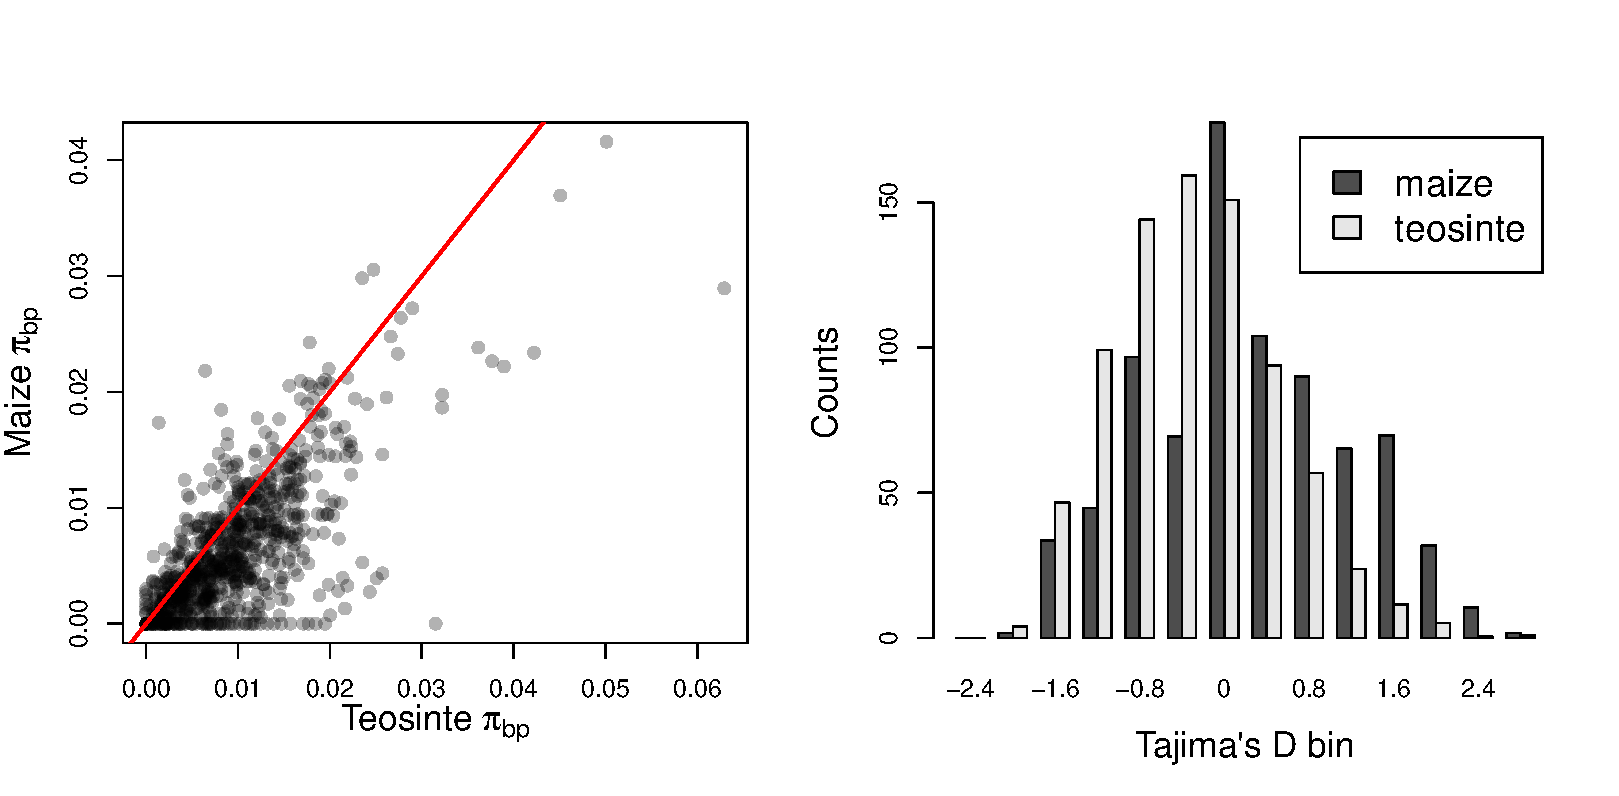
\includegraphics[width = \textwidth]{Journal_figs/genetic_drift/Maize_bottleneck/Wright_Tajima_D.pdf}
\end{center}
\caption[][-2cm]{Data for polymorphism from Maize and Teosinite: 774
  genes redrawn from \citet{Wright:05}. {\bf Left)} Genetic  diversity levels in maize and and Teosinte samples at each of these genes.
Note how diversity levels are lower in maize than teosinte, i.e. most
points are below the red $x=y$ line. {\bf Right)} The distribution of Tajima's D in maize and teosinte, see how the maize distribution is shifted towards positive values. \gitcode{} } \label{fig:maize_Tajimas_D}  %é
\end{figure}

\begin{marginfigure}[4cm]
\begin{center}
  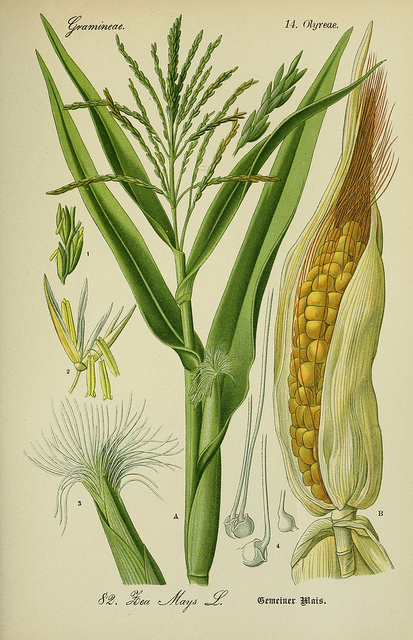
\includegraphics[width = \textwidth]{illustration_images/Genetic_drift/maize/7845339168_66aa3d8ccc_z.jpg}
\end{center}
\caption{Maize ({\it Zea mays}.) \BHLNC{Prof. Dr. Thomé's Flora von
  Deutschland. 1886. Thomé, O. W.}{https://www.biodiversitylibrary.org/page/12306602\#page/669/mode/1up}{New York Botanical Garden}} \label{fig:maize}  %é
\end{marginfigure}  %%possible different fig https://peerj.com/preprints/26502.pdf from Jeff's paper

Mutations that arise on deeper lineages will be at intermediate frequency in our sample, and so mild bottlenecks
can lead to an excess of intermediate frequency alleles compared to
the standard constant-population model. This can skew 
Tajima's D, see eqn \ref{eqn_Tajimas_D}, towards positive values and away from its expectation of
zero . One example of this skew is shown in Figure
\ref{fig:maize_Tajimas_D}. Maize ({\it (Zea mays} subsp.{\it mays}) was domesticated from its wild progenitor teosinte ({\it (Zea mays
subsp. parviglumis}) roughly ten thousand years ago. We can see how the
 bottleneck associated with domestication has resulted in a loss of genetic diversity in maize, compared to teosinte, and the polymorphism that remains is somewhat skewed towards intermediate frequencies resulting in more positive values of Tajima's D.

\begin{question}
\citet{voight2005interrogating} sequenced 40 autosomal regions from 15 diploid samples of Hausa people from Yaounde, Cameroon. The average length of locus they sequenced for each region was $2365$bp. They found that the average number of segregating sites per locus was $S= 11.1$ and the average $\pi = 0.0011$ per base over the loci. Is Tajima's D positive or negative? Is a demographic model with a bottleneck or growth more consistent with this result?
\end{question}





\section{Molecular Evolution and the fixation of neutral alleles} 
\begin{quote}
"history is just one damn thing after another" -Arnold Toynbee 
\end{quote} %https://quoteinvestigator.com/2015/09/16/history/

It is very unlikely that a rare
neutral allele accidentally drifts up to fixation; more likely, such an allele
will be eventually lost from the population. However, populations experience a
large and constant influx of rare alleles due to mutation, so even if it is
very unlikely that an individual allele fixes within the population, some
neutral alleles will fix by chance. \\


%We'll first consider the probability that a neutral allele fixes
%within the population, starting from it just enters a diploid
%population as a newly mutated allele at frequency $1/(2N)$.

%so for an allele to be fixed in the population it
%must have been that allele

\paragraph{Probability of the eventual fixation of a neutral allele}
% TODO: tried to clean up this section, needs more work
\begin{figure}
\begin{center}
  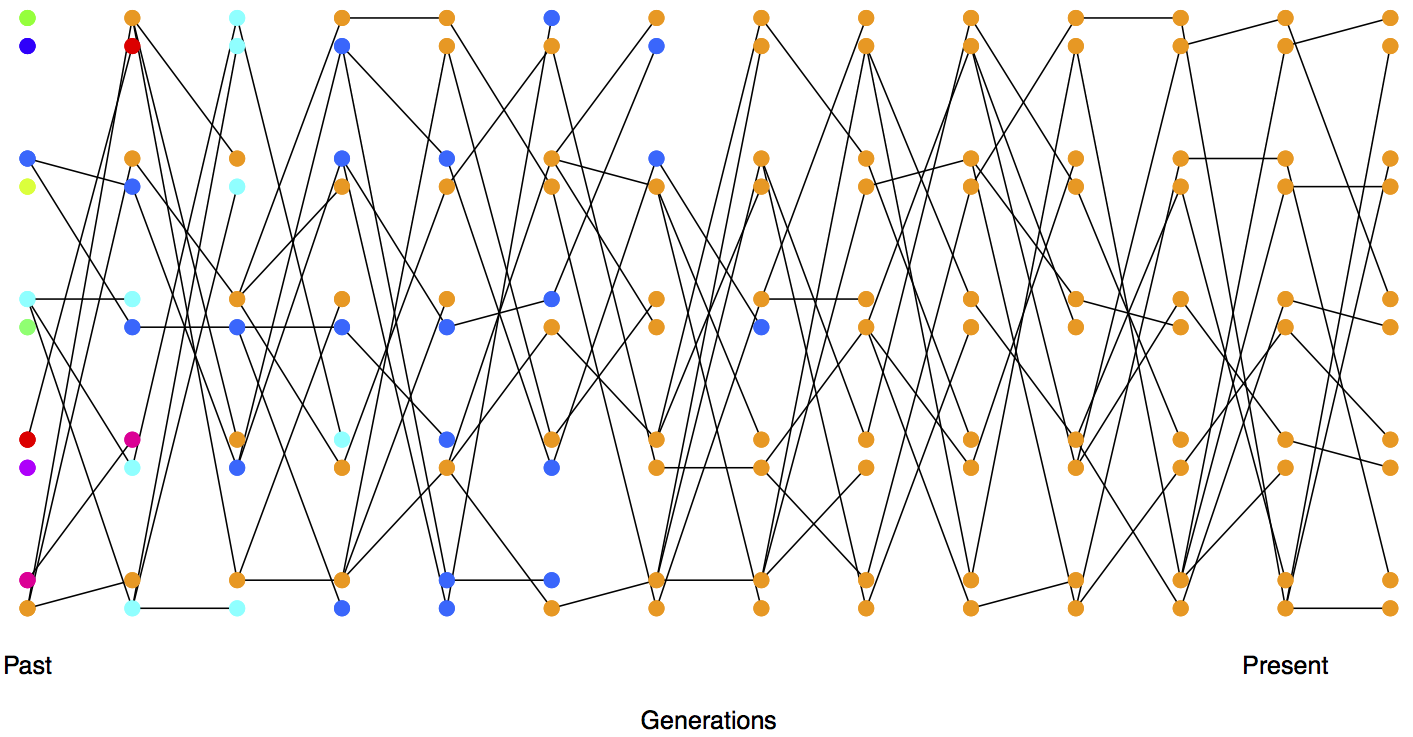
\includegraphics[width = \textwidth]{figures/Substitution_sim.png}
\end{center}
\caption{Each allele initially present in a small diploid population is
  given a different colour so we can track their descendants over
  time. By the 9th generation, all of the alleles present in the
  population can trace their ancestry back to the orange allele. \gitcode{https://github.com/cooplab/popgen-notes/blob/master/Rcode/Loss_of_heterozyg_varying_pop.R}} \label{fig:subs_simulation}
\end{figure}

An allele which reaches fixation within a population is an ancestor to the
entire population. In a particular generation there can only be a single allele
that all other alleles at the locus in a later generation can claim as an
ancestor (See Figure \ref{fig:subs_simulation}). At a neutral locus, the actual allele does not affect the number of
descendants that the allele has (this follows from the definition of
neutrality: neutral alleles don't leave more or less descendants on average than other neutral alleles).
An equivalent way to state this is that the allele labels don't affect
anything; thus the alleles are \emph{exchangeable}. As a consequence of being exchangeable,
any allele is equally likely to be the ancestor of the entire population.  In a
diploid population of size $N$, there are $2N$ alleles, all of which are
equally likely to be the ancestor of the entire population at some later time
point. So if our allele is present in a single copy, the chance that it is the
ancestor to the entire population in some future generation is
$\nicefrac{1}{(2N)}$, i.e. the chance our neutral allele is eventually fixed is
$\nicefrac{1}{(2N)}$.  In Figure \ref{fig:subs_simulation}, our orange allele
in the first generation is one of 10 differently coloured alleles, and so has a
$1/10$ chance of being the ancestor of the entire population at some later time
point (and in this simulation it does become the common ancestor, by the 9th generation).\\

More generally, if our neutral allele is present in $i$ copies in the
population, of $2N$ alleles, the probability that this allele becomes fixed is
$\nicefrac{i}{(2N)}$, i.e. the probability that a neutral allele is eventually
fixed is simply given by its frequency ($p$) in the population.  (We can also
derive this result by letting $Ns \rightarrow 0$ in eqn.
\eqref{eqn:prob_fixed}, a result we'll encounter later.)




% TODO
A newly arisen mutation only becomes a fixed difference if it is lucky
enough to be the ancestor of the entire population. As we saw above, this occurs
with probability $\nicefrac{1}{(2N)}$. 

How long does it take on average for
such an allele to fix within our population? Well, in developing
equation \eqref{TMRCA_neutral} we've seen that it takes $4N$
generations for a large sample of alleles to all trace their ancestry back to a
single most recent common ancestral allele. Any single-base pair change which arose as a single mutation at a locus, and fixed in the population, must have been present in the sequence transmitted by the most recent common ancestor of the population at that locus. Thus it must take roughly $4N$ generations
for a neutral allele present in a single copy within the population to the
ancestor of all alleles within our population.  This argument can be made more
precise, but in general we would still find that it takes $\approx 4N$
generations for a neutral allele to go from its introduction to fixation with
the population.   \\

\paragraph{Rate of substitution of neutral alleles}

A substitution between populations that do not exchange gene flow is simply a
fixation event within one population. The rate of substitution is therefore the
rate at which new alleles fix in the population, so that the long-term
substitution rate is the rate at which mutations arise that will eventually
become fixed within our population.\\

Lets assume, based on our discussion of the neutral theory of molecular evolution, that there are only two classes of mutational changes that can occur with a
region, highly deleterious mutations and neutral mutations. A fraction $C$ of
all mutational changes are highly deleterious, and cannot possibly contribute
to substitution nor polymorphism.  The other $1-C$ fraction
of mutations are neutral. If our mutation rate is $\mu$ per transmitted allele
per generation, then a total of $2N \mu (1-C)$ neutral mutations enter our
population each generation.\\

Each of these neutral mutations has a $\nicefrac{1}{(2N)}$ probability chance of
eventually becoming fixed in the population. Therefore, the rate at
which neutral mutations arise that eventually become fixed within our
population is  
\begin{equation}
2N\mu(1-C)\frac{1}{2N} = \mu(1-C)
\end{equation}
Thus the rate of substitution, under a model where newly arising alleles are either
highly deleterious or neutral, is simply given by the mutation rate
of neutral alleles, i.e. $\mu(1-C)$.\\

Consider a pair of species that have diverged for $T$ generations, i.e. orthologous sequences shared between the species last shared a common ancestor $T$ generations ago. If these species have maintained a constant $\mu$ over that time, they will have accumulated an average of
\begin{equation}
2\mu(1-C)T \label{eqn:moleclock}
\end{equation}
neutral substitutions. This assumes that $T$ is a lot longer than the time it
takes to fix a neutral allele, such that the total number of 
alleles introduced into the population that will eventually fix is the
total number of substitutions.\\

This is a really pretty result as the population size has completely canceled
out of the neutral substitution rate. However, there is another way to see this
in a more straight forward way. If I look at a sequence in me compared to, say, a
particular chimp, I'm looking at the mutations that have occurred in both of
our germlines since they parted ways $T$ generations ago. Since neutral alleles
do not alter the probability of their transmission to the next generation, we
are simply looking at the mutations that have occurred in $2T$ generations
worth of transmissions. Thus the average number of neutral mutational
differences separating our pair of species is simply $2\mu (1-C) T$.\\

\marginnote{\begin{quote}"functionally less important molecules or parts of a molecule
evolve faster than more important ones." \end{quote} -- \citet{kimura1974some}}
A number of observations follow under this model, from equation \eqref{eqn:moleclock}, the first is that a primary determinant of patterns of molecular evolution in a genomic region is the level of constraint ($C$). This pattern generally seems to hold empirically: non-coding regions often evolve more rapidly than coding regions; synonymous substitutions accumulate faster than nonsynonymous; nonsynonymous changes faster in less vital proteins than ones that are absolutely necessary for early development. Note that this is not a unique prediction of the neutral model, e.g. lower pleiotropy means that less constrained regions may be better able to evolve adaptively. However, it is a fantastically useful general insight, e.g. it allows us to spot putatively functional non-coding regions by looking for genomic regions that have very low levels of divergence among distantly related species.

\begin{figure}
\begin{center}
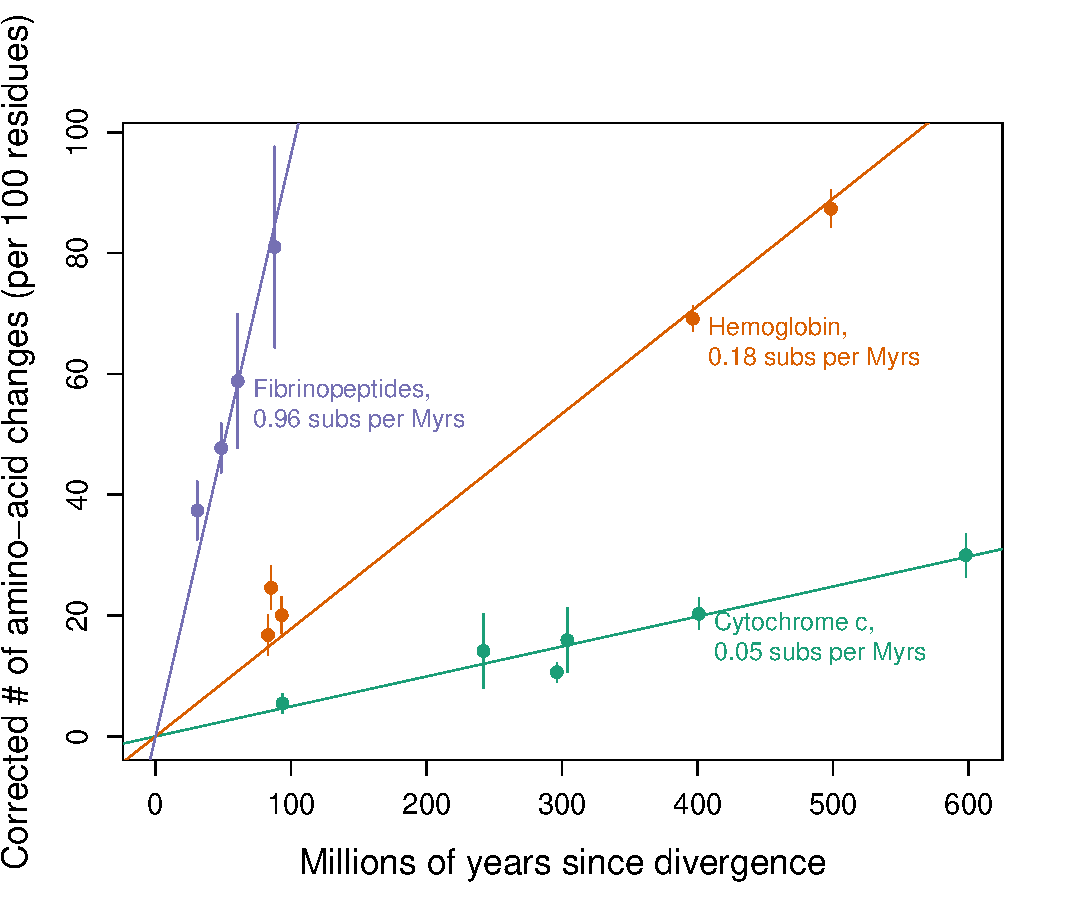
\includegraphics[width=0.8 \textwidth]{Journal_figs/genetic_drift/Molecular_clock_Dickerson/Dickerson_1979_mole_clock_fig.pdf}
\end{center}
\caption{The numbers of substitutions between various pairs of groups, for three proteins, plotted against the time these groups shared a common ancestor in the fossil record. Data from  \citet{dickerson1971structure}. The number of observed amino-acid differences is corrected for multiple hits to obtain the corrected number of changes estimated to occur. The lines give the linear regression, constrained to pass through the origin, for each protein. The slope of the regression is given next to the protein name. \gitcode{https://github.com/cooplab/popgen-notes/blob/master/Journal_figs/genetic_drift/Molecular_clock_Dickerson/Dickerson_1979_mole_clock_data.R} See \citep{robinson2016revisiting} who revisited this classic study and confirmed the conclusions.} \label{fig:Dickerson_mole_clock}  
\end{figure}

\begin{marginfigure}[-1cm]
\begin{center}
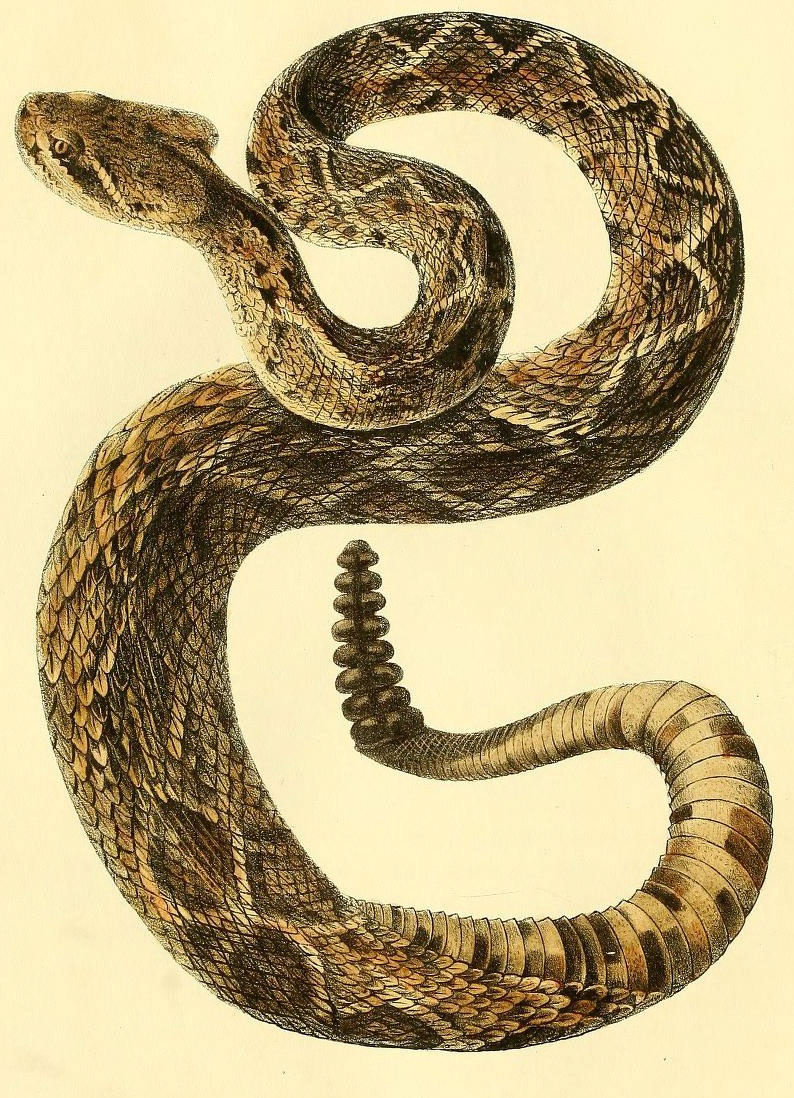
\includegraphics[width= 0.8 \textwidth]{illustration_images/Genetic_drift/rattlesnake/rattlesnake.jpg}
\end{center}
\caption{Eastern diamondback rattlesnake ({\it Crotalus adamanteus}. \BHLCC{North American herpetology. Holbrook, J. E. }{https://www.biodiversitylibrary.org/page/35765722\#page/120/mode/1up}{Smithsonian Libraries}{2.0} } \label{fig:rattlesnake}  
\end{marginfigure}

The second important insight, and critical for the development of the neutral theory, is that equation \eqref{eqn:moleclock} is seemingly consistent with \citet{zuckerkandl1965evolutionary}'s hypothesis of a surprisingly constant, protein molecular clock. The protein molecular clock is the observation that for some proteins there's a linear relationship between the number of non-synonymous substitutions and the time species last shared a common ancestor in the fossil record. \citet{dickerson1971structure} provided an for early example of this observation (Figure \ref{fig:Dickerson_mole_clock}), by comparing various organisms whose molecular sequences were available to him. For example, he found that humans and rattlesnakes, who last share a common ancestor in the fossil record around 300 million years, are separated by roughly $15$ NS substitutions per $100$ sites in the Cytochrome c protein.
While, humans and dog fish, which diverged around 400 million years, are separated by $19$ NS substitutions per $100$ sites in this gene. \\ \graham{add dog fish pic? https://www.flickr.com/photos/biodivlibrary/sets/72157645618396122/ Added molecular clock question} 

In equation \eqref{eqn:moleclock} we double the amount of time separating a pair of species $T$, we double the number of substitutions predicted. Note that for this to be true $T$ must be measured in generations. To explain a protein molecular clock between species that clearly differed dramatically in generation time it was hypothesized that the mutation rate actually scaled with generation time, i.e. short-lived organisms introduced less mutations per generation, e.g. as they had fewer rounds of mitosis. This generation-time assumption meant that the mutation rate per year could be constant, such that $\mu T$ would be a constant for pairs of species that had diverged for similar geological times, which are measured in years, even if the organisms differed in generation time. This assumption would allow neutral theory to be consistent with a protein molecular clock measured in years. We now know that this critical generation time assumption is false, organisms with shorter generation times have somewhat higher mutation rates per year, and so a strict neutral model is inconsistent with the protein molecular clock. We'll return to these ideas when we discuss the fate of very weakly selected mutations in Chapter \ref{Selection_Stochasticity} and \citet{ohta1973slightly}'s Nearly Neutral theory. If you are still reading this send Graham a picture of Tomoko Ohta receiving the Crafoord Prize, an analog of the Nobel prize for biology, for her contributions to molecular evolution. \graham{I currently dont do generation time effect in that chapter, need to update}
\graham{add side note on adjustment for multiple hits'}
\graham{add note about fibrinogen having non-essential spacer pepitides}


\paragraph{The contribution of ancestral polymorphism to divergence.} If we are considering $T$ to represent the divergence between long-separated species, then we can think of $T$ as the time that the
species split. However, for more recently diverged populations and
species, we need to include the fact that the sorting of ancestral
polymorphism contributes to divergence among species. In Figure 
\ref{fig:split_anc_pop}, we see our two populations split $T_s$ generations ago.  However, the
coalescence of our A and B lineage is necessarily deeper in time than
$T_s$. The top mutation was polymorphic in the ancestral population
but now contributes to the divergence between A and B. Assuming that
our ancestral population had effective size $N_A$ individuals, and
that our populations split cleanly with no subsequent gene flow, then
\begin{equation}
T = T_s + 2N_A.
\end{equation}
If our species split time is very large compared to $2N$ then we can think of $T$ as the split time. 

\begin{marginfigure}
\begin{center}
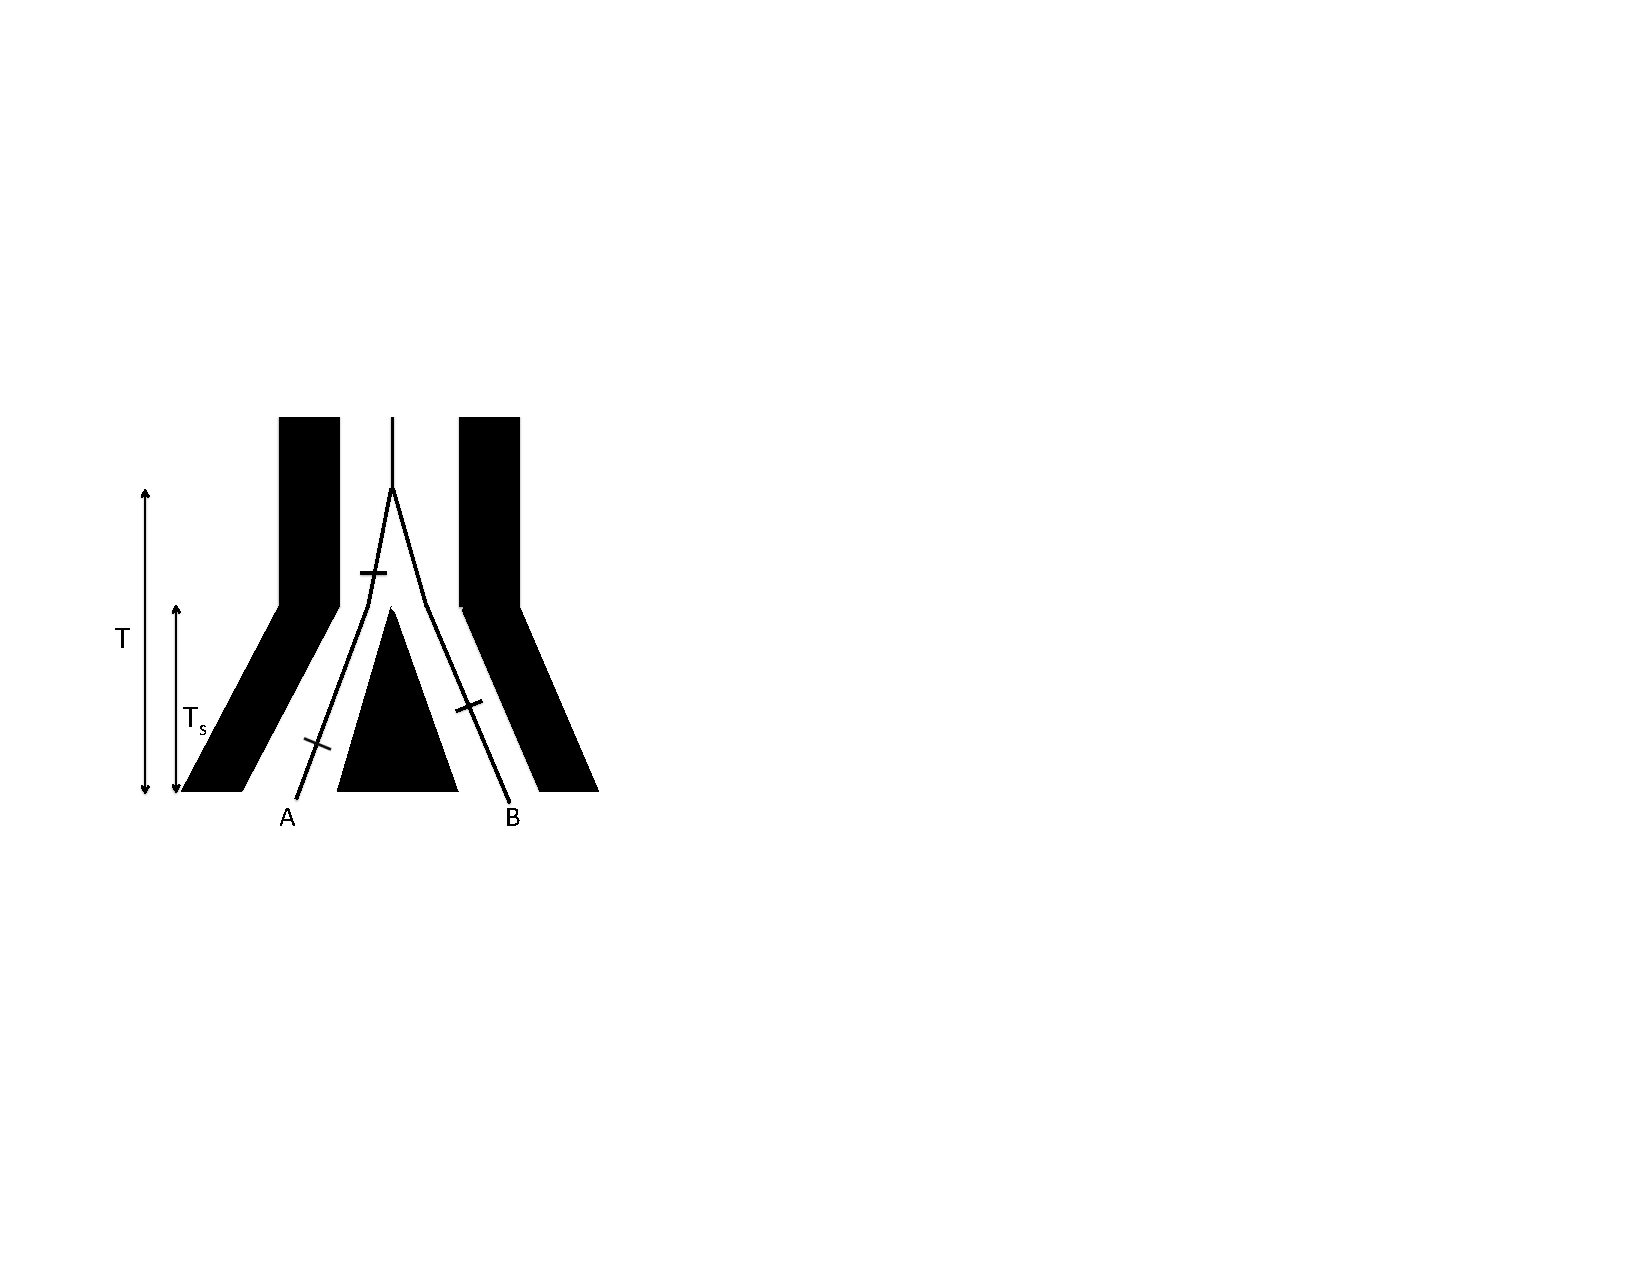
\includegraphics[width=0.8 \textwidth]{figures/Genetic_drift/ILS/split_anc_pop.pdf}
\end{center}
\caption{The genealogy of two alleles one sampled from population A and B. Mutations on the lineages are shown as dashes. The pair of alleles coalesce in the ancestral population of A and B. The two populations split $T_S$ generations ago, with no subsequent gene flow, but the two lineages must coalesce deeper in time. } \label{fig:split_anc_pop}  
\end{marginfigure} 

\graham{update numbers in Q}
%Our expected number of substitutions is scaling linearly with our species $T$ split time measured in generations.  

%\erin{I think this last concept is hard and may be a bit confusing for students without some additional pictures or text} %\graham{lineup split time in this section w. FST section.}



\begin{question}
For this, and the next question, assume that humans and chimp diverged
%\graham{Update numbers?}
around 5.5$\times 10^6$ years ago, have a generation time ~20 years, that the speciation occurred instantaneously in allopatry with no subsequent gene flow, and the ancestral effective population size of the human and chimp common ancestor population was 10,000 individuals.\\
Nachman and Crowell sequenced 12 pseudogenes in human and chimp and found substitutions at 1.3\% of sites. \\
{\bf A) } What is the mutation rate per site per generation at these genes?\\
{\bf B)} All of the pseudogenes they sequenced are on the autosomes. What
would your prediction be for pseudogenes on the X and Y chromosomes,
given that there are fewer rounds of replication in the female
germline than in the male germline.
\end{question}

\section{Tests of molecular evolution.}

\subsection{Comparing the rates of non-synonymous to synonymous
substitutions $\dNdS$}
One common tool in molecular evolution is to compare the estimated number (or rates) of substitutions in different classes of genomic sites, for example the ratio of the number of non-synonymous to synonymous substitutions in a given gene. The simplest way to calculate $d_N$ is to 
count up the non-synonymous changes and divide by the total number of
positions in the gene where a non-synonymous point mutation could occur. We
can do likewise for synonymous changes $d_S$, and then take the ratio $\dNdS$. This is a helpful
conceptual way to think about what $\dNdS$ represents, however, this
ignores the fact that some changes are more likely to occur by
mutation than others and also does not account for multiple hits (multiple mutations at the same bp position). Therefore, in
practice the ratio $\dNdS$ is more typically calculated by model-based
likelihood and bayesian methods
that can account for these features. 

For the vast majority of protein-coding genes in the genome we see that $\dNdS < 1$. This observation is consistent with the view
that non-synonymous sites are much more constrained than synonymous sites, i.e. that most non-synonymous mutations are deleterious and quickly removed from the population. If we are willing to make the assumption that all synonymous changes are
neutral, $d_S=2T \mu$, then we can estimate the degree of constraint on non-synonymous sites. (Note that synonymous changes can sometimes be subject to
both positive and negative selection, but this neutral assumption is a useful starting place.) 

Assume that a fraction $C$ of non-synonymous changes are too
deleterious to contribute to polymorphism. Then, after $T$ generations of divergence have
elapsed between two populations, we'd expect $d_N$ neutral non-synonymous substitutions, where
\begin{equation}
d_N = 2T (1-C) \mu  
\end{equation}
Dividing by $d_S$, we find
\begin{equation} 
\dNdS = (1-C) 
\end{equation}
Therefore, if we assume that non-synonymous mutations can only be
strongly deleterious or neutral, we estimate the fraction of mutational changes that
are constrained by negative selection as $C= 1- \dNdS$. C has the
interpretations of being the fraction of non-synonymous mutations that are quickly weeded out of the population by selection, and so do not contribute to divergence among species. 

We can test whether our gene is evolving in a constrained way at the protein level by estimating $\dNdS$ and testing whether this is significantly less that  $1$. A $\dNdS$ test can provide evolutionary evidence that a stretch of DNA proposed to be protein-coding is subject to selective constraint, and so likely does encode for a functional protein. We can also perform a $\dNdS$ test on specific branches of a phylogeny for a gene, to test on which branches the gene is subject to constraint, or to test for changes in the level of constraint across the phylogeny.

\graham{add pic of distribution of dN/dS}

\paragraph{Loss of constraint at pseudogenes.}


\marginnote{
``Rudimentary organs may be compared with the letters in a word, still
retained in the spelling, but become useless in the pronunciation, but
which serve as a clue .. for its derivation.''  -- \citet{darwin1859} pg. 455
}  %http://darwin-online.org.uk/Variorum/1859/1859-456-dns.html

While most protein genes evolve under constraint, we can find examples of
genes that are evolving in a less constrained manner. The simplest
example of this is where the gene has lost function. Genes can lose function because of inactivating mutations that stop them being transcribed or translated into functional proteins. Such genes are called 'pseudogenes'. When a gene completely loses function there is no longer
selection against non-synonynous changes and so such mutations are just as free
to accumulate as synonymous changes, and so $\dNdS=1$.
Pseudogenes are a wonderful example of the extension of Darwin's ideas about vestigial traits (`Rudimentary organs') to the DNA level;
we can still recognize a once useful word (gene) whose spelling is slowly degrading. Our genomes are filled with old pseudogenes whose
original meanings (functional protein coding sequences) are slowly being eroded through the accumulation of neutral substitutions.
One nice example of a gene that has repeatedly lost function,
i.e. become repeatedly psuedogenized, is
the Enamlin gene from the study of \citet{Meredith:09}.

\begin{figure}
\begin{center}
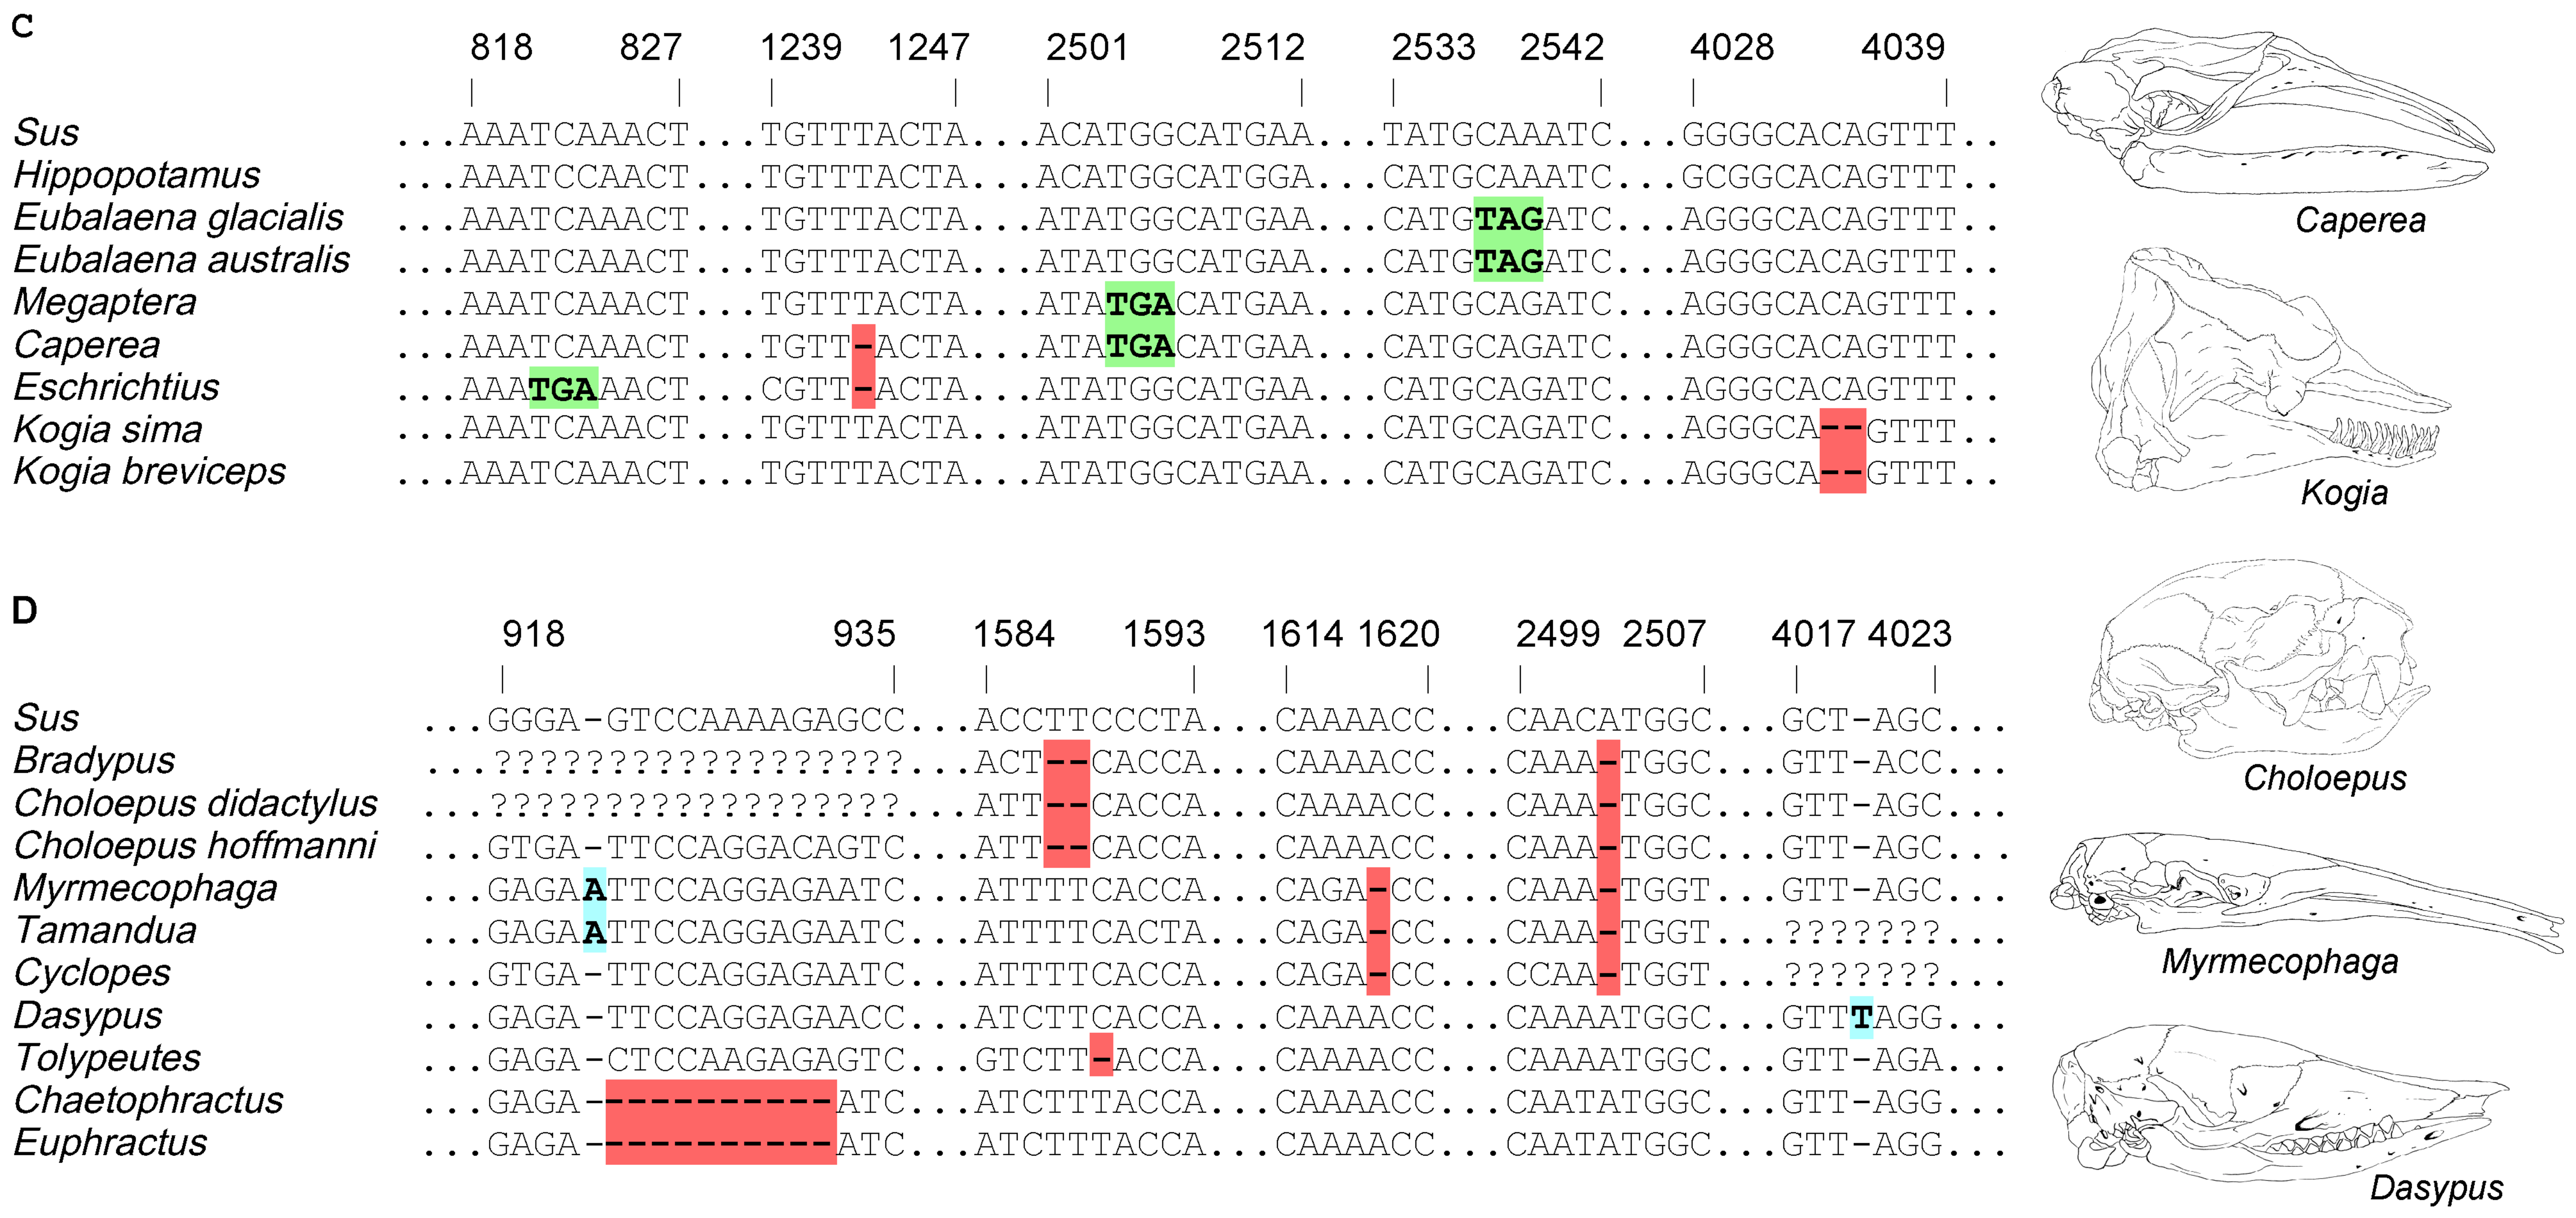
\includegraphics[width=\textwidth]{Journal_figs/genetic_drift/Enamelin/Enamlin.pdf}
\end{center}
\caption{Examples of frameshift mutations (insertions blue, deletions
  red) and premature stop codons in Enamlin in Cetacea and
  Xenarthra. Figure from \citet{Meredith:09}, \PLOSccBY. } \label{fig:Enamlin_coding}  
\end{figure} 

\begin{marginfigure}
\begin{center}
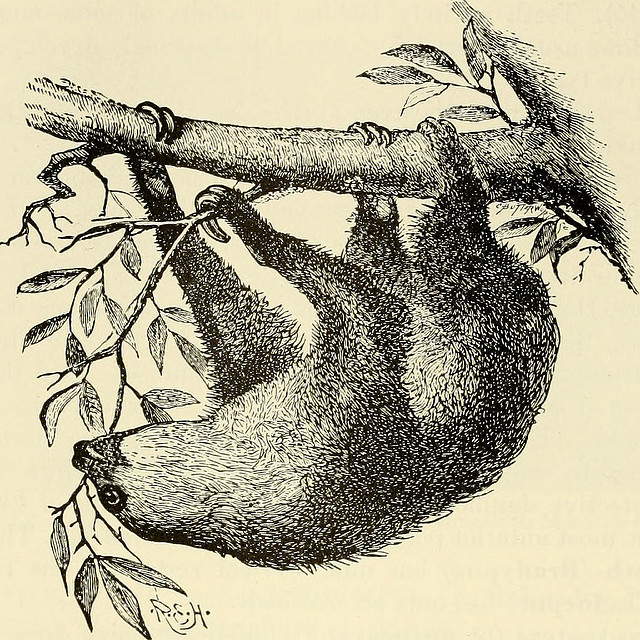
\includegraphics[width=\textwidth]{illustration_images/Genetic_drift/sloth/20423856040_6e4360df9c_z.jpg}   %https://www.biodiversitylibrary.org/page/39742681#page/1005/mode/1up
\end{center}
\caption{Two-toed sloth ({\it Choloepus hoffmanni}). \BHLNC{An introduction
  to the study of mammals, living and extinct. 1891. Flower W. H. and Lydekker R.}{https://archive.org/stream/chordates00rand/\#page/744/mode/1up}{University of Toronto} } \label{fig:sloth}  
\end{marginfigure} 

The protein Enamlin is a key structural protein involved in the outer cap of enamel on teeth. Various mammals have secondarily evolved diets that do not require hard teeth, and so greatly reduced the selection pressure for hard enamel, or even teeth at all. For example, two-toed sloths ({\it Choloepus}), Pygmy sperm whales ({\it Kogia}), and aardvark {\it Orycteropus}) all lack  enamel on teeth. Other mammals have lost their teeth entirely, e.g. giant anteaters ({\it Myrmecophaga}) and Baleen whales. Due to this relaxation of constraint on the phenotype, the Enamlin gene has accumulated pseudogenizing substitutions such as premature stop codons and frameshift mutations (see Figure \ref{fig:Enamlin_coding}
for examples).  \citeauthor{Meredith:09} sequenced Enamlin across a
range of species and found that none of the species with enamel have frameshift
mutations in Enamlin, while 17/20 of species that lack enamel or teeth have
frameshifts in Enamlin, and all of them carry premature stop codons
(Figure \ref{fig:Enamlin_phylo}). 

\begin{figure}
\begin{center}
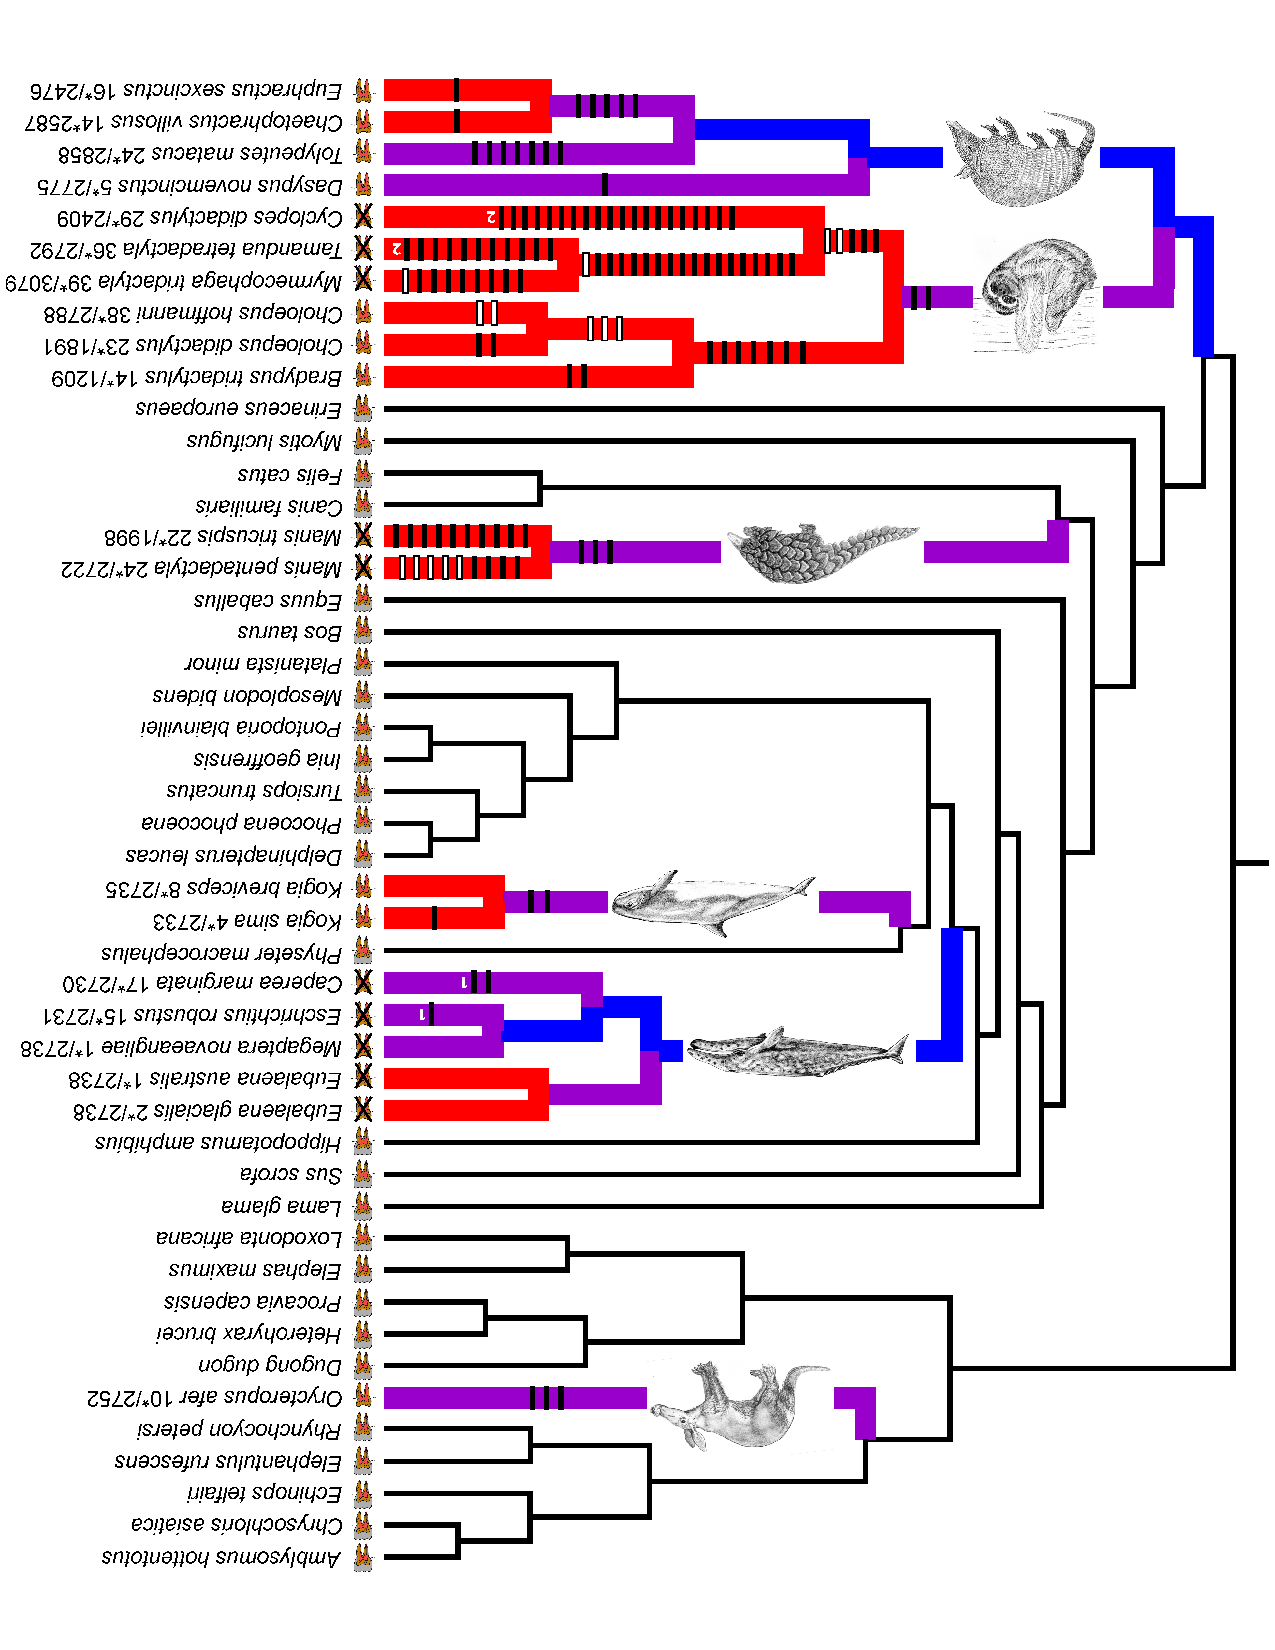
\includegraphics[width= \textwidth]{Journal_figs/genetic_drift/Enamelin/Enamlin_phylo.pdf}
\end{center}
\caption{The tooth symbol next to each taxon shows whether they have
  teeth with enamel, lack enamel, or lack teeth. Branches of the phylogeny are coloured by whether their
  Enamlin is functional (black), pre-mutation (blue), mixed (purple), or pseudogenic (red). The black and white vertical bars on branches show frameshift
  mutations.  The numbers after taxon names indicate minimum number of
  stop codons in the sequence divided by  the length of the sequence. Figure from \citet{Meredith:09}, \PLOSccBY.} \label{fig:Enamlin_phylo}  
\end{figure} 

The branches of the Enamlin phylogeny with a functional Enamlin gene (black) had an estimated $\dNdS= 0.51$, consistent with the protein evolving in a constrained manner. In contrast, the branches with a pseudogenized Enamlin (red)
had $\dNdS = 1.02$, consistent with the gene evolving an unconstrained
way. The branches where the gene was likely transitioning from a functional
to non-function state, i.e. pre-mutation (blue) and mixed (purple), had intermediate values of
$\dNdS=0.83-0.98$, consistent with a transition from a constrained to unconstrained mode of protein evolution somewhere along these branches of the phylogeny.

%\begin{question}
%Enamlin was pseudogenized somewhere along the branch leading to
%Aardvarks ({\it Orycteropus}). This branch has $\dNdS=0.75$
% https://journals.plos.org/plosgenetics/article?id=10.1371/journal.pgen.1000634#pgen.1000634.s007
%dawn pangloin
%https://commons.wikimedia.org/wiki/File:Eomanis_waldi_4.jpg
%% aadvark https://www.flickr.com/photos/internetarchivebookimages/20514695666/in/photolist-xfPbiq-xUcng7-xCyGQA-xdRRQ3-wPMGZr-tFgYfN-wPMPkT-tDahHQ-xuc4KM-xKR4u3-xUkupQ-w88zeU-xMia2r-sp4Aq5-x1wNyZ-xMi46D-tDaCr7-sJE2X4-tFB8Lc-wHWiNj-tp8AUk-tFvh4R-xu3M7w-toUVwN-wYWgVi-w34vHn-x9xAfL-wWhnso-ovvmHE-tG5AgB-xdUzWD-y82dEG-xCA7kx-xV5xWg-wYc33H-wYbFdX-wYbBMP-xUcjpL-xKQjHw-xJmBQU-xKPwEQ-xLEzv4-xu3wHJ-xLEg9V-xnA6Lr-x684wQ-wZNgpq-wYcVbh-wZtb3F-wYbJLh
%%% w1 t/T + w2(T-t)/T = wT
%% https://journals.plos.org/plosgenetics/article?id=10.1371/journal.pgen.1000634#pgen.1000634.s007



%\end{question}
\paragraph{Adaptive evolution and $\dNdS$.}
Clearly genes are not only subject to neutral and deleterious mutations; beneficial mutations must also arise and fix from from time to time. 
Let's assume that a fraction $B$ of non-synonymous mutations that arise are
beneficial such that $2 N \mu B$ beneficial mutations arise per generation. Newly arisen beneficial alleles are not destined to fix in the population, as they may be lost to genetic drift when they are rare in the population (we'll
discuss how to calculate the fixation probability for beneficial
alleles in Chapter \ref{Selection_Stochasticity}). A newly arisen beneficial allele reaches fixation in the population with probability $f_B$ from its initial frequency of $\nicefrac{1}{2N}$. This fixation
probability may be much higher than that of neutral mutations, but still much less than $1$.  If $2T$ generations of divergence have
elapsed between the two populations then a total of
\begin{equation}
dN=2T (1-C - B) \mu  + 2T \times (2 N \mu B) \times  f_B
\end{equation}
non-synonymous substitutions will have accumulated.
Then
\begin{equation} 
\dNdS = (1-C-B) +  2 N B f_B
\end{equation}
assuming again that all synonymous mutations are neutral. Note that this means that our estimates of $C$ using $1-\dNdS$ will be
a  lower bound on the true constraint if even a small fraction of
mutations are beneficial. Those cases where the gene is evolving more rapidly at the protein level than at synonymous
sites, i.e. $d_N/d_S > 1$, are potentially strong candidates for  positive selection rapidly driving change at the protein level. We can identify genes that have $\dNdS$ significantly greater than one, either on the complete gene phylogeny, or on particular branches. Note that is a very conservative test that few genes in the genome meet, as many genes that are fixing adaptive non-synonymous substitutions will have $\dNdS<1$;  even if adaptive mutations are common, genes may still evolve in a constrained way (i.e. $\dNdS<1$) if
the rapid fixation of beneficial mutations due to positive selection is outweighed by the loss of non-synonymous mutations to negative selection.

% \paragraph{loss of constraint} While most genes evolve under constraint, we can find examples of
% genes that are evolving in a less constrained manner. The simplest
% example of this is where the gene has lost function, e.g. has recently
% become pseudogenized. Along branches of the phylogeny where all the
% constraint against non-synonymous mutation has
% been lost then $\dNdS=1$. We can also identify cases where the gene
% is evolving more rapidly at the protein level than at synonymous
% sites, i.e. $d_N/d_S > 1$, corresponding to cases of rapid change due
% to positive selection. 

\begin{figure}
\begin{center}
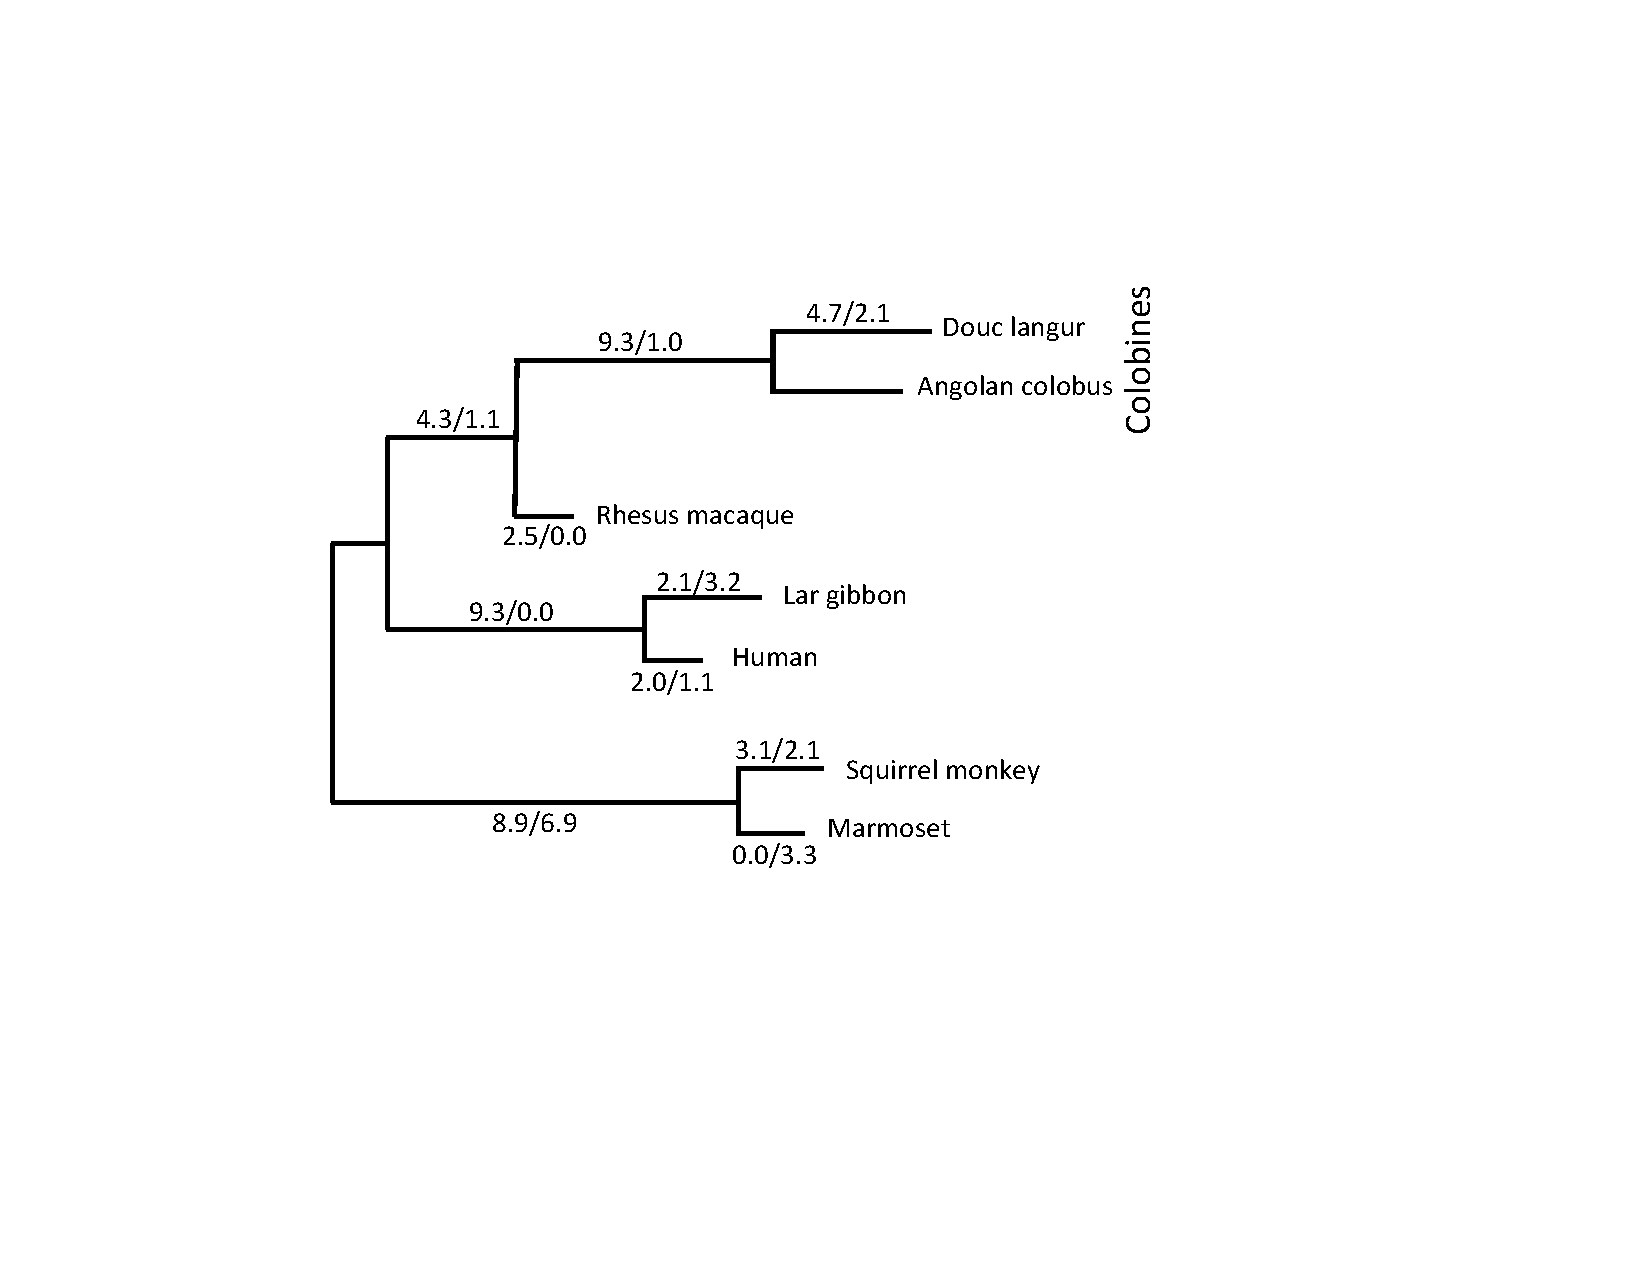
\includegraphics[width=0.8 \textwidth]{Journal_figs/genetic_drift/Yang_lysozyme/Yang_lysozyme.pdf}
\end{center}
\caption{A phylogram for the primate lysozyme gene, data from
  \citet{Yang:98}. For each branch, the numbers give the estimated average
number of non-synonymous to synonymous changes in the lysozyme protein.} \label{fig:lysozyme}  
\end{figure} 

\begin{marginfigure}
\begin{center}
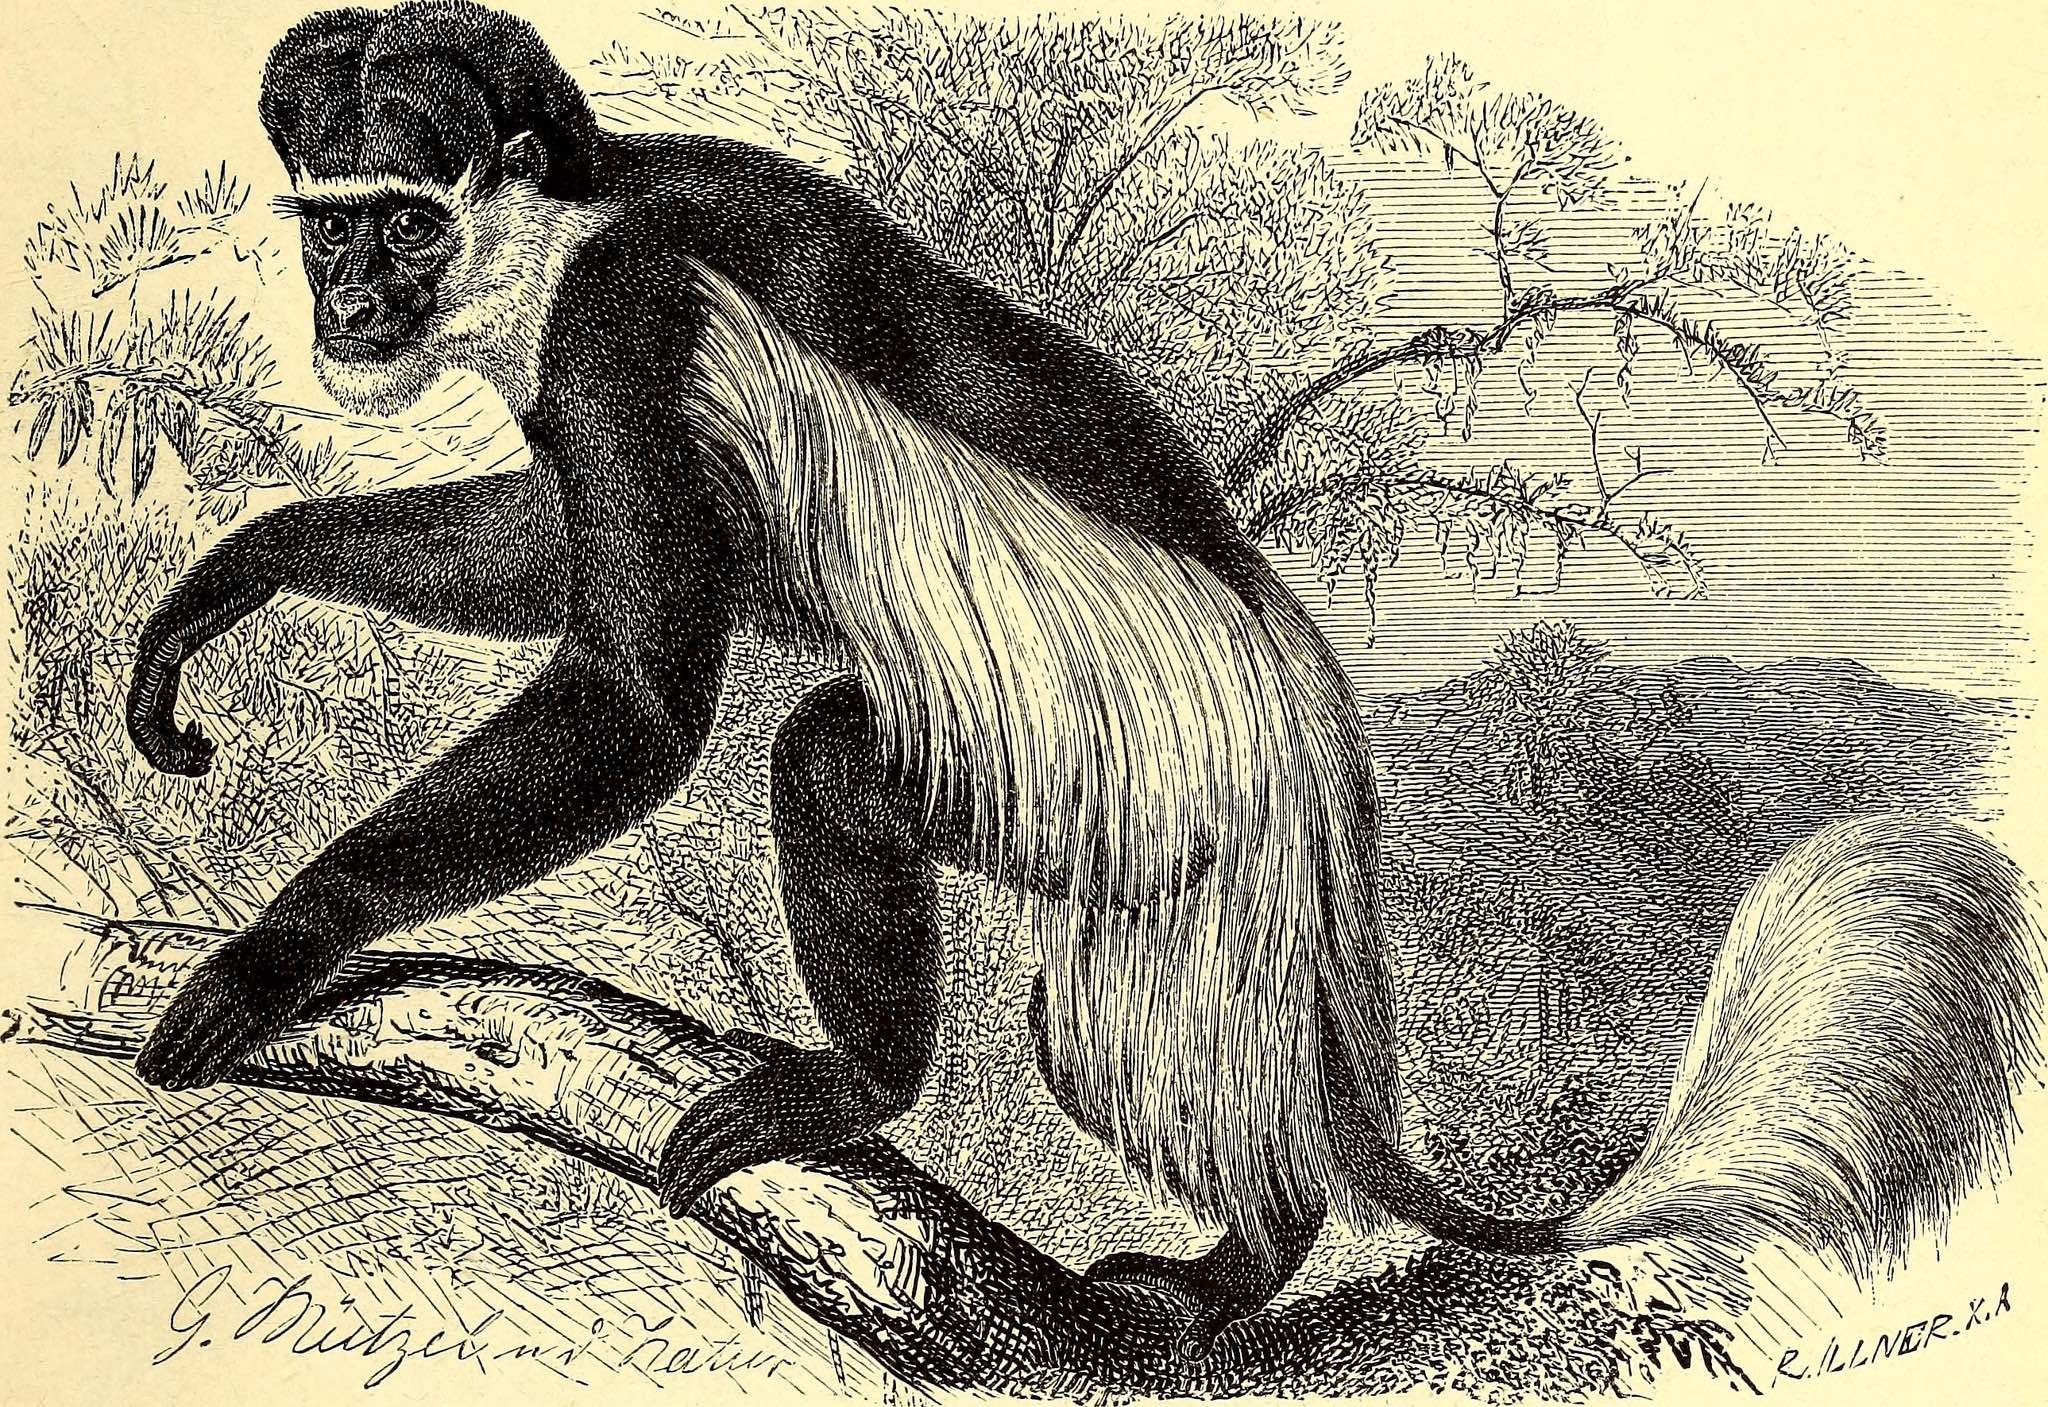
\includegraphics[width=0.8 \textwidth]{illustration_images/Genetic_drift/Colobus/19792029373_fcce706e67_k.jpg}
\end{center}
\caption{Abyssinian black-and-white colobus ({\it Colobus guereza}). A member of the leaf-eating Colobines. \BHLNC{Brehm's Tierleben,  Brehm,
  A.E. 1893.}{https://archive.org/stream/brehmstierlebena001breh/\#page/125/mode/1up}{University of Illinois Urbana-Champaign}} \label{fig:Colobus}  
\end{marginfigure} 

\begin{marginfigure}
\begin{center}
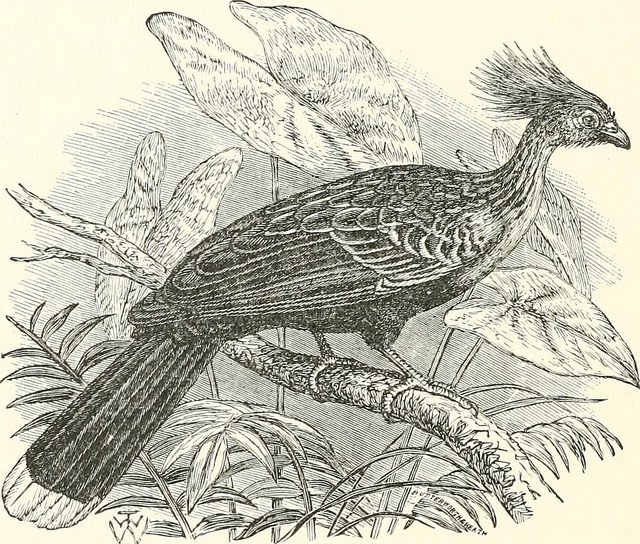
\includegraphics[width=0.8  \textwidth]{illustration_images/Genetic_drift/Hoatzin/14747388314_85798ba97e_z.jpg}
\end{center}
\caption{ (hoatzin ({\it Opisthocomus hoazin}). A leaf-eating bird. \BHLNC{A history of birds (1910)
  Pycraft, W.P.}{https://archive.org/stream/historyofbirds00pycr/historyofbirds00pycr\#page/238/mode/1up}{ American Museum of Natural History Library}} \label{fig:hoatzin}  
\end{marginfigure} 
A classic example for looking at adaptive evolution using dN/dS is the
evolution of the lysozyme protein in primates \citep{Messier:97,Yang:98}, see
the phylogeny in Figure \ref{fig:lysozyme}. The lysozyme protein is
a key component for the breakdown of bacterial walls. It shows very
fast protein evolution, notably on the lineages leading to apes (e.g. gibbons
and humans) and Colobines (e.g. colobus and langur monkeys). Colobines have leaf-based diets. They digest
these leaves by bacterial fermentation in their foregut, and then use lysozymes to break down the bacteria to extract energy from the
leaves. In Colobines, the lysozyme protein has evolved to work well in the high-PH environment of the stomach. Remarkably, the Colobine
lysozyme has convergently evolved this activity via very similar amino-acid changes at 5 key residuals in cows and Hoatzins \citep[a leaf
eating bird,][]{kornegay1994molecular} 

\paragraph{The Mcdonald-Kreitman test}

As noted above, a big issue with using $\dNdS$ to detect adaptation is that it is very conservative. For a more powerful test of rapid divergence, what we need to do is adjust for the level of constraint a gene experiences at non-synonymous sites. One way to do this is to use polymorphism data as an internal control. If we see little non-synonymous polymorphism at a gene, but a  lot of synonymous polymorphism, we now know that there is likely strong constraint on the gene (i.e. high $C$), thus we expect $\dNdS$ to be low. \citet{mcdonald:91} devised a simple test of the neutral theory of molecular evolution at a gene based on this intuition \citep[building on the conceptually similar HKA
test][]{hudson1987test}. \citeauthor{mcdonald:91} took the case where we have polymorphism data at a gene for one species and divergence to a closely related species. They  partitioned polymorphism and fixed differences in their sample into 
non-synonymous and synonymous changes:

\begin{center}
\begin{tabular}{ccc}
 & Poly. & Fixed \\
\hline 
Non-Syn. &    $P_N$  &   $D_N$  \\
Syn. &    $P_S$   &     $D_S$   \\
Ratio & $P_N/P_S$ & $D_N/D_S$
\end{tabular}
\end{center}

\begin{marginfigure}
\begin{center}
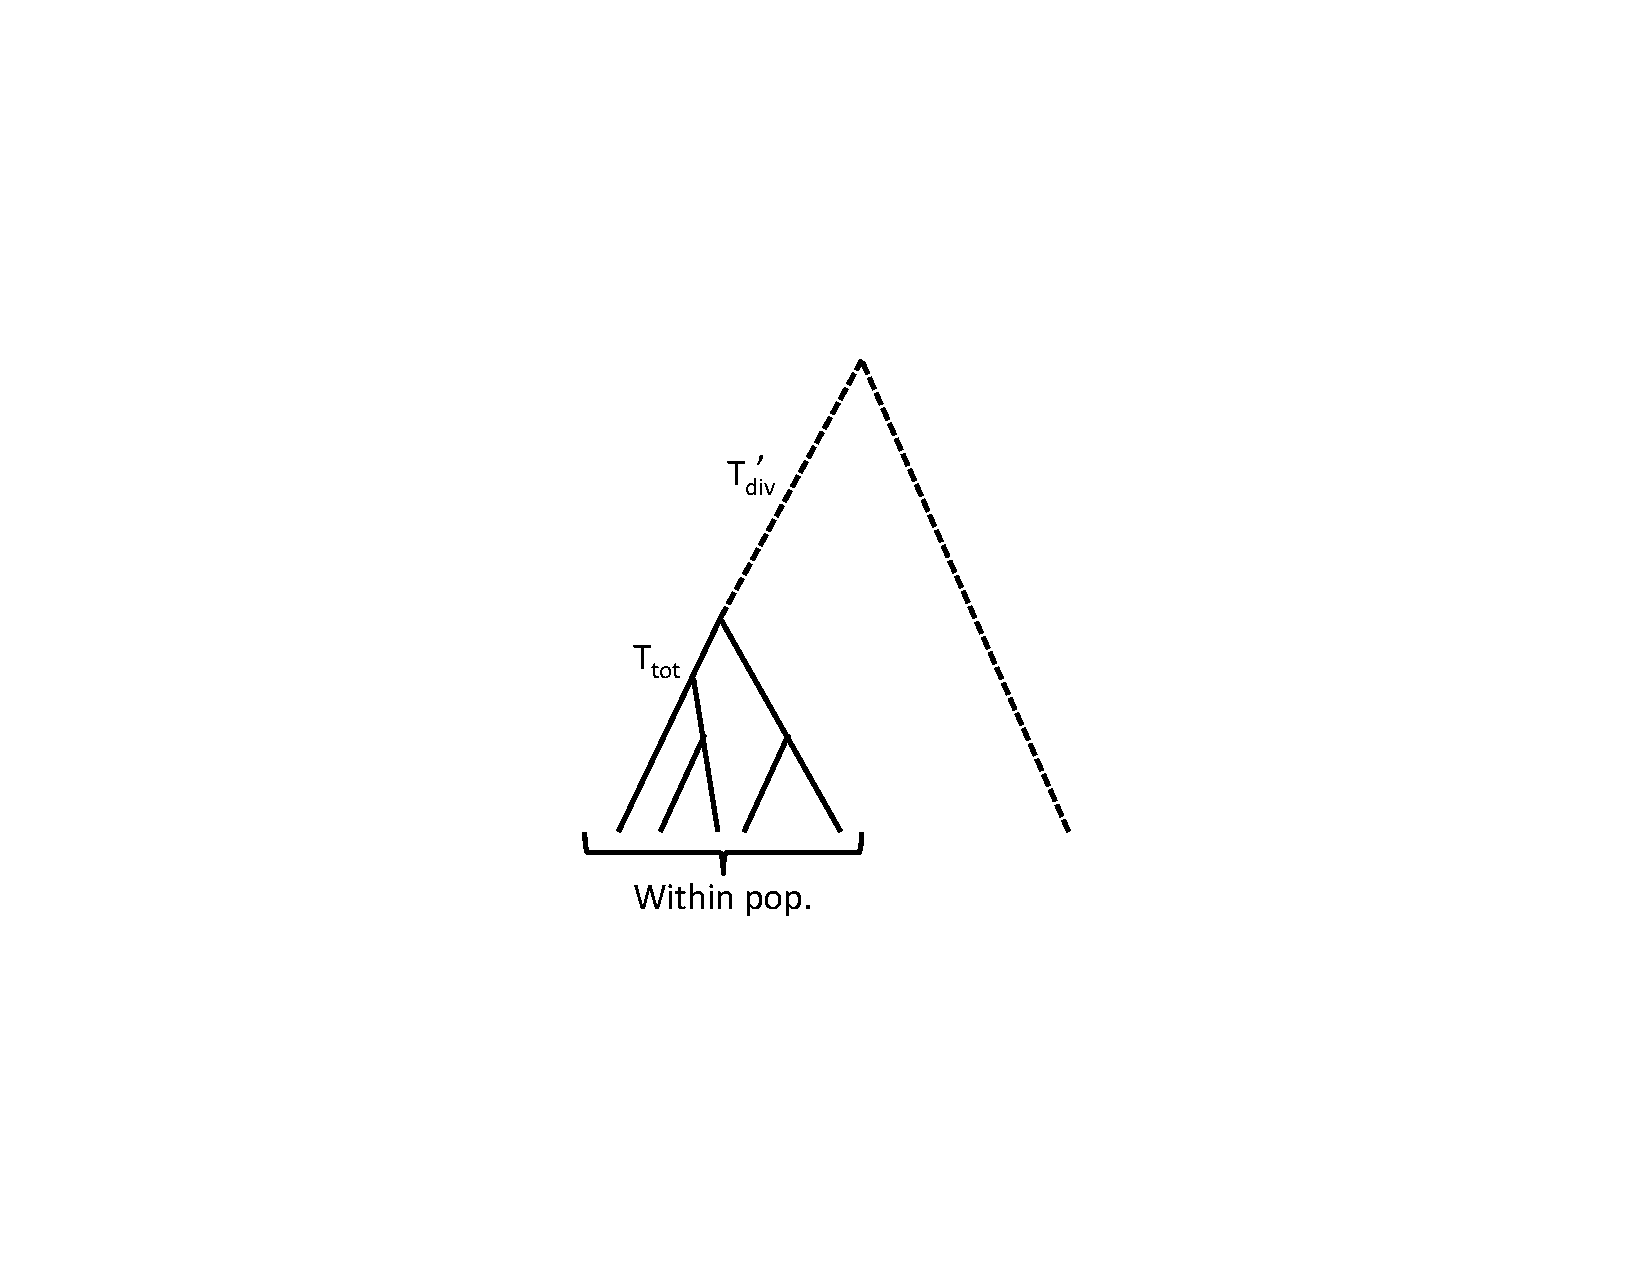
\includegraphics[width= \textwidth]{figures/Coalescent/MK_tree.pdf}
\end{center}
\caption{An example ogene genealogy for a set of alleles sampled within a population and a single allele sampled from a distantly-related species.} \label{fig:MK_tree}
\end{marginfigure}

Under neutral theory, we expect a smaller number of non-synonymous to
synonymous fixed differences ($D_N/D_S < 1$) and exactly the same
expectation holds for polymorphism ($P_N/P_S$). Let's consider a gene with $L_S$ and $L_N$ sites where synonymous and non-synonymous mutations could arise respectively. 
We can think of the underlying gene genealogy at our gene, see Figure \ref{fig:MK_tree}, with the total time on the coalescent genealogy within the species as $T_{tot}$ and the total time for fixed differences between our species as $T_{div}'$. Then under neutrality we expect $ \mu L_N (1-C) T_{tot}$
non-synonymous polymorphisms (i.e. our number of segregating sites), and  $ \mu L_N (1-C) T_{div}'$ non-synonymous fixed differences. We can then fill out the rest of our table as follows: 


\begin{center}
\begin{tabular}{ccc}
 & Poly. & Fixed  \\
 \hline
Non-Syn. &    $\mu L_N (1-C) T_{tot}$  &   $\mu L_N (1-C)  T_{div}'$ \\
Syn. &    $\mu L_N T_{tot}$   &     $\mu L_S T_{div}'$  \\
Ratio & $ L_N(1-C)/( L_S)$  & $ L_N (1-C) / ( L_S)$
\end{tabular}
\end{center}
Therefore, we expect the ratio of non-synonymous to synonymous changes to be the same for polymorphism and divergence under a strict neutral model. We can test this expectation of equal ratios via the standard tests of a $2
\times 2$ table. If the ratio of $N/S$ is significantly higher for divergence than polymorphism we have evidence that non-synonymous substitutions are accumulating more rapidly than we would predict given levels of constraint alone.

\begin{marginfigure}
\begin{center}
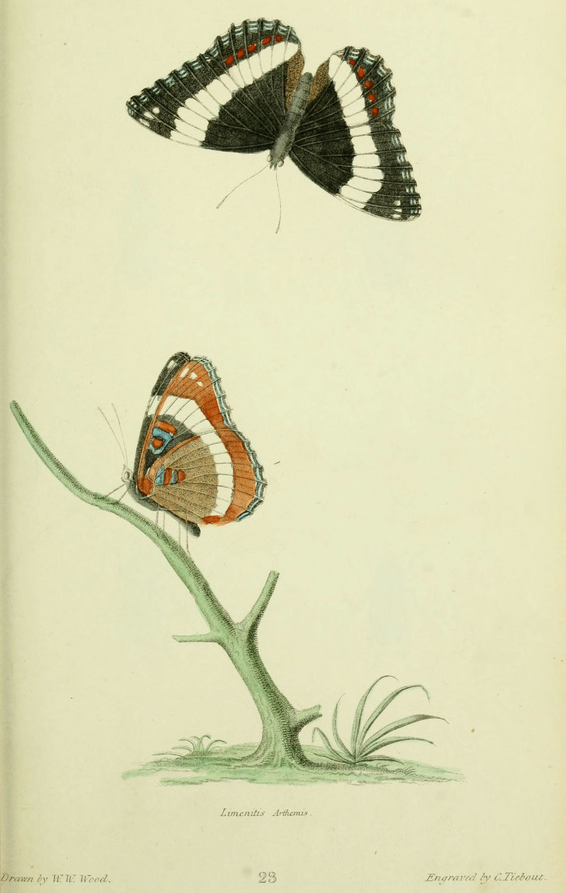
\includegraphics[width= \textwidth]{illustration_images/Genetic_drift/Limenitis_arthemis/Limenitis.png}
\end{center}
\caption{White admiral ({\it Limenitis arthemis}). \BHLNC{American entomology : a description of the insects of North American (1859). Say, T. }{https://www.biodiversitylibrary.org/page/9194935\#page/487/mode/1up}{Smithsonian Libraries}} \label{fig:Limenitis}
\end{marginfigure}
As example of a Mcdonald-Kreitman table consider the work of \citet{frentiu2007adaptive} on the molecular evolution of L Photopigment opsin in Admiral
({\it Limenitis}) butterflies, responsible for colour vision in the long-wavelength part of the visual spectrum. \citeauthor{frentiu2007adaptive} found that the sensitivity of this opsin had shifted towards blue-shifted in its sensitivity in {\it L. archippus archippus} (viceroy) compared to {\it  L. arthemis astyanax}. To test whether this molecular evolution reflected positive selection they sequenced  24 {\it L. arthemis astyanax} individuals and one {\it  L. archippus archippus} sequence. They identified  11 polymorphic sites in  {\it L. arthemis astyanax} and 16 fixed differences, which break down as follows:
\begin{center}
\begin{tabular}{ccc}
 & Poly. & Fixed  \\
 \hline
Non-Syn. &    $2$  &   $12$ \\
Syn. &    $9$   &     $4$  \\
Ratio & $\nicefrac{2}{9}$  & $\nicefrac{3}{1}$
\end{tabular}
\end{center}
Note the strong excess of non-synonymous to synonymous divergence compared to polymorphism (p-value of $0.006$, Fisher's exact test), which is consistent with the gene evolving in an adaptive manner among the two species. We would expect roughly only $3$ non-synonymous substitutions out of 16 substitutions if the gene was evolving neutrally ($ 16 \times \nicefrac{2}{11}$). 

% \graham{add  Adriana Briscoe butterfly eye eg}  %https://twitter.com/AdrianaBriscoe/status/1057205734407094272 

\section{Neutral diversity and population structure}
%% this section was moved from the coalescent chapter
We've considered alleles drawn from a randomly-mating population, and divergence among alleles drawn from two distantly-related populations. 
We'll now turn to consider divergence among more closely related populations. In thinking about the coalescent  within populations we made the assumption that any pair of lineages is equally likely to coalesce with each
other. However, when there is population structure this assumption is violated. \\

We have previously written the measure of population structure
$\fst$ as
\begin{equation}
\fst = \frac{H_T-H_S}{H_T}
\end{equation}
where $H_S$ is the probability that two alleles sampled at random from a
subpopulation differ, and $H_T$ is the probability that two alleles
sampled at random from the total population differ. 

\paragraph{A simple population split model}
Imagine a population of constant size of $N_e$ diploid individuals that
$T$ generations in the past split into two daughter populations (sub-populations)
each of size $N_e$ individuals, which do not subsequently exchange
migrants. In the current day we sample an equal number of alleles
from both subpopulations. 

\begin{figure}
\begin{center}
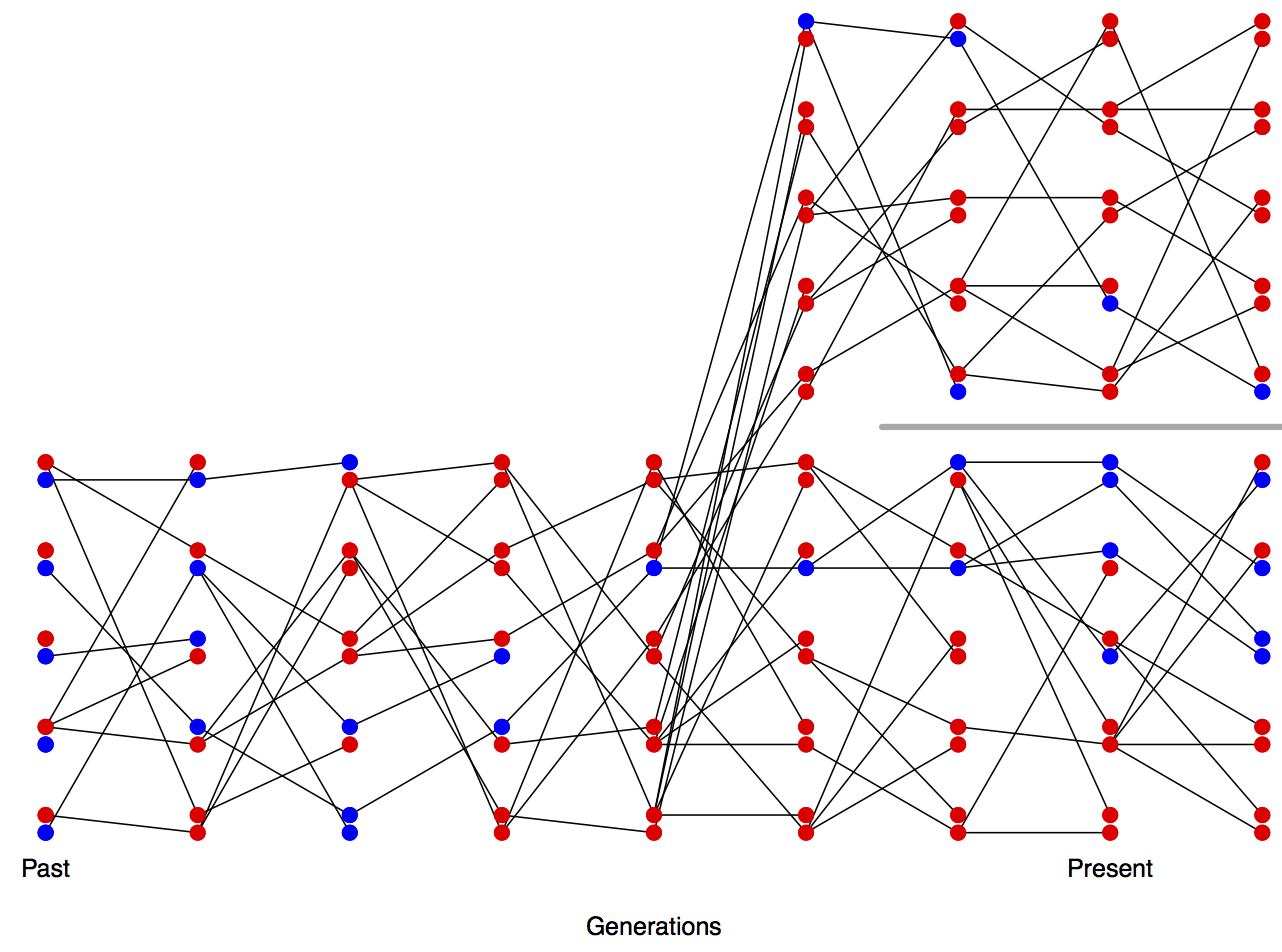
\includegraphics[width= 0.8 \textwidth]{figures/drift_split.png}
\end{center}
\caption{Change in allele frequencies following a population split. \gitcode{https://github.com/cooplab/popgen-notes/blob/master/Rcode/Loss_of_heterozyg_varying_pop.R}} \label{fig:drift_split}  
\end{figure} 

Consider a pair of alleles sampled within one of our
sub-populations and think about their per site heterozygosity. 
These alleles have experienced a population of size $N_e$
and so the probability that they differ is $H_S \approx 4N_e \mu$ (assuming that $N_e \mu \ll 1$, using our equation  \ref{eqn:hetero} for heterozygosity within a population ).

%Consider a pair of alleles sampled within one of our
%sub-populations, they have experienced a population of size $N_e$
%and so the probability that they differ is $H_S = \theta/(1+\theta)$
%(where $\theta=4N_e\mu$).


The heterozygosity in our total population is a little more tricky to
calculate. Assuming that we equally sample both sub-populations, when we draw two alleles from our total
sample, $50\%$ of the time they are drawn from the same
subpopulation and $50\%$ of the time they are drawn from different
subpopulations. Therefore, our total heterozygosity is given by
\begin{equation}
H_T = \half H_S + \half H_B
\end{equation}
where $H_B$ is the probability that a pair of alleles drawn from our
two different sub-populations differ from each other. A pair of
alleles from different sub-populations cannot find a common ancestor with each other for at least $T$
generations into the past as they are in distinct populations (not
connected by migration). Once our alleles find themselves back in the combined ancestral 
population it takes them on average $2N$ generations to coalesce. So the total opportunity for mutation between our pair of alleles sampled from different populations is $2 (T + 2N )$ generations of meioses, such that the probability that our pairs of alleles is different is 
\begin{equation}
H_B \approx 2\mu ( T + 2 N) %\left( 1-(1-\mu)^{2T} \right) + (1-\mu)^{2T}
  %\frac{\theta}{\theta+1} 
\end{equation}


%The probability that one or other of them
%mutates in this time is $1-(1-\mu)^{2T}$. With probability
%$(1-\mu)^{2T} $ neither of our alleles mutate in the $T$ generations
%back in time before they find themselves back in the combined ancestral 
%population. Conditional on failing to mutate before the combined ancestral
%population, the probability that they do manage to mutate before
%coalescing in that population of size $N_e$ is
%$\theta/(\theta+1)$. Putting these components together
%\begin{equation}
%H_B = \left( 1-(1-\mu)^{2T} \right) + (1-\mu)^{2T}
 % \frac{\theta}{\theta+1} 
%\end{equation}
We can plug this into our expression for $H_T$, and then that in turn
into $\fst$. Doing so we find that
\begin{equation}
\fst \approx \frac{ \mu T}{\mu T +  4N_e\mu }  = \frac{ T}{ T +  4N_e }
\end{equation}
Note that $\mu$ cancels out of this equation. In this simple toy model, $\fst$
is increasing because the amount of between-population diversity 
increases with the divergence time of the two populations (initially
linearly with $T$). $\fst$ grows at a rate
give by $\nicefrac{T}{(4N_e)}$ so that differentiation will be higher
between populations separated by long divergence times or with small
effective population sizes.

\begin{marginfigure}
\begin{center}
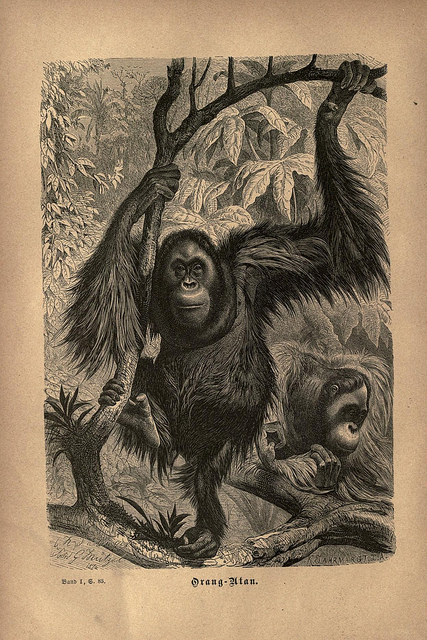
\includegraphics[width= 0.8 \textwidth]{illustration_images/Genetic_drift/Orang/7971889392_d32b45668b_z.jpg}
\end{center}
\caption{Orangutan ({\it Pongo}). \BHLNC{Brehms thierleben, allgemeine kunde des thierreichs. Brehm, A. E.}{https://www.biodiversitylibrary.org/page/1008013\#page/114/mode/1up}{MBLWHOI Library}} \label{fig:Orang}  
\end{marginfigure} 


\begin{question}  %Pongo abelii (Sumatran) and Pongo pygmaeus
  The genome-wide $F_{ST}$ between Bornean and Sumatran orang-utan species samples  ({\it Pongo pygmaeus} and {\it Pongo abelii}) is $\approx 0.37$ \citep{locke2011}, representing a deep population split between the species (potentially with little subsequent gene flow). Within the populations the genome-wide average Watterson's $\theta$ is $\theta_W=1.4$kb$^{-1}$, estimated from the number of segregating sites. Assume a generation time of 20 years, and a mutation rate of $2 \times 10^{-8}$ per base per generation. How far in the past did the two populations diverge?
\end{question}
%o understand this better we can make a simple
%approximation based on our mutation rate being very low, such that
%$N_e \mu \ll 1$ so $H_S \approx
%4N_e\mu$, and that $\mu \ll 1$ and $\mu T \ll 1$. Assuming this, then  
%\begin{equation}
%H_B \approx 2 \mu T + 4N_e\mu. 
%\end{equation}



%\begin{question}
%The gorilla lineage split from the human-chimp lineage $\sim$7 million years ago. Let’s assume that this speciation event occurred instantaneously in allopatry with no subsequent gene flow. \\
%{\bf A)}	What is the probability of that gorilla is not an outgroup to human and chimp at a single locus?\\
%{\bf B)}	It has been estimated that the gorilla lineage is not an outgroup at around ~30\% of autosomal loci. What effective population size would you need to assume to explain this observation? Is that only plausible explanation?\\
%{\bf C)}	The gorilla lineage is an outgroup for large portions of the X chromosome, what is a plausible explanation for this finding?
%\end{question}

\paragraph{A simple model of migration between an island and the mainland.}
We can also use the coalescent to think about patterns of
differentiation under a simple model of migration-drift
equilibrium. Let's consider a small island population that is relatively isolated
from a large mainland population, where both of these populations
are constant in size. We'll assume that the expected heterozygosity
for a pair of alleles sampled on the mainland is $H_M$.

Our island has a population size
$N_{I}$ that is very small compared to our mainland population.
Each generation some low fraction $m$ of our individuals on the
island have migrant parents from the mainland the generation
before. Our island may also send migrants back to the mainland, but
these are a drop in the ocean compared to the large population size on
the mainland and their effect can be ignored. 


If we sample an allele on the island and trace its ancestral
lineage backward in time, each generation our ancestral allele has a low
probability $m$ of being descended from the mainland in the preceding
generation (if we go back far enough the allele eventually has to be
descended from an allele on the mainland). The probability that a pair of alleles sampled on the
island are descended from a shared recent common ancestral allele on the island is the
probability that our pair of alleles coalesces before either lineage
migrates. For example, the probability that our pair of alleles
coalesces $t+1$ generations back on the island is 
\begin{equation}
\frac{1}{2N_I}(1-m)^{2(t+1)} \left(1-\frac{1}{2N_I} \right)^{t} \approx
\frac{1}{2N_I} \exp\left( -t\left (\frac{1}{2N_I} + 2m\right) \right),
\end{equation}
with the approximation following from assuming that $m \ll 1$ \& $\frac{1}{(2N_I)}
\ll 1$ (note that this is very similar to our derivation of
heterozygosity above). The probability that our alleles coalesce before either one
of them migrates off the island, irrespective of the time, is
\begin{equation}
\int_0^{\infty} \frac{1}{2N_I} \exp\left( -t\left (\frac{1}{2N_I} +
2m\right) \right) dt = \frac{\nicefrac{1}{(2N_I)}}{\nicefrac{1}{(2N_I)} +
    2m}.
\end{equation}

Let's assume that the mutation rate is very low such that it is very
unlikely that the pair of alleles mutate before they coalesce on the
island. Therefore, the only way that the alleles can be different from
each other is if one or other of them migrates to the mainland, which
happens with probability  
\begin{equation}
  1 - \frac{\nicefrac{1}{(2N_I)}}{\nicefrac{1}{(2N_I)} + 2m}
\end{equation}
Conditional on one or other of our alleles migrating to the mainland, both of our alleles represent independent draws from the mainland and so differ from each other with probability $H_M$. Therefore, the level of
heterozygosity on the island is given by
\begin{equation}
  H_I = \left(1 - \frac{\nicefrac{1}{(2N_I)}}{1/(2N_I) + 2m} \right)H_M
\end{equation}
So the reduction of heterozygosity on the island compared to the
mainland is
\begin{equation}
  F_{IM} = 1- \frac{H_I}{H_M} = \frac{\nicefrac{ 1}{(2N_I)}}{\nicefrac{1}{(2N_I)} + 2m} = \frac{ 1 }{1 + 4N_Im}.
\end{equation}
The level of inbreeding on the island compared to the mainland will be high if the migration rate is low and the effective population size of the island is low, as allele frequencies on the island are drifting and diversity on the island is not being replenished by migration. The
key parameter here is the number individuals on the island replaced by immigrants from the mainland each generation ($N_I m$).

We have framed this problem as being about the reduction in genetic diversity on the island compared to the mainland. However, if we consider collecting individuals on the island and mainland in proportion to their population
sizes, the total level of heterozygosity would be $H_T=H_M$, as samples from our mainland would greatly outnumber those from our island. Therefore, considering the island as our sub-population, we have derived another simple model of $F_{ST}$.

\begin{question}
You are investigating a small river population of sticklebacks, which receives infrequent migrants from a very large marine population. At a set of putatively neutral biallelic markers the freshwater population has frequencies:\\
0.2, 0.7, 0.8\\
at the same markers the marine population has frequencies:\\
0.4, 0.5 and 0.7.\\
 From studying patterns of heterozygosity at a large collection of markers, you have estimated the long term effective size of your freshwater population is 2000 individuals.\\
What is your estimate of the migration rate from the marine
populations into the river?
\end{question}

\paragraph{Incomplete lineage sorting}

Because it can take a long time for an polymorphism to drift up or down in frequency, multiple population splits may occur during the time an allele is still segregating. This can lead to incongruence between the overall population tree and the information about relationships present at
individual loci. In Figure \ref{fig:NoILS_poly} and \ref{fig:ILS_poly}
we show a simulations of three populations where the bottom population splits off from the other two first, followed by the subsequent splitting of the the top and the middle populations. We start both simulations with a newly
introduced red allele being polymorphic in the combined ancestral population. The most likely fate of this allele is that it is
quickly lost from the population, but sometimes the allele can drift up in frequency and be polymorphic when the populations split, as the alleles in our two figures have done. If the allele is lost/fixed in the descendant populations before the next population split, our allele
configuration will agree with the population tree, as it does in
Figure  \ref{fig:NoILS_poly}, and so too the gene tree will agree with population tree (as shown in the left side of Figure \ref{fig:ILS_cartoon}). 
However, if the allele persists as a polymorphism in the ancestral population till the top and the middle
populations split, then the allele can fix in one of these populations
and not the other. Such an event can lead to a substitution pattern
that disagrees with the population tree, as in Figure \ref{fig:ILS_poly}.  If
we were to construct a phylogeny using the variation at this site we would see a disagreement between the gene tree and population tree. In Figure \ref{fig:ILS_poly} an allele
drawn from the top and the bottom populations are
necessarily more closely related to each other than either is to an allele drawn from population 2; 
tracing our allelic lineages from the top and bottom populations back through time, they must coalesce with each other before we reach the point where the red mutation arose; in contrast, a lineage from the middle population cannot have coalesced with either other lineage until past the time the red mutation arose. An example of this 'incomplete lineage sorting' in terms of the underlying tree is shown on the right side of Figure \ref{fig:ILS_cartoon} . 


\begin{figure}
\begin{center}
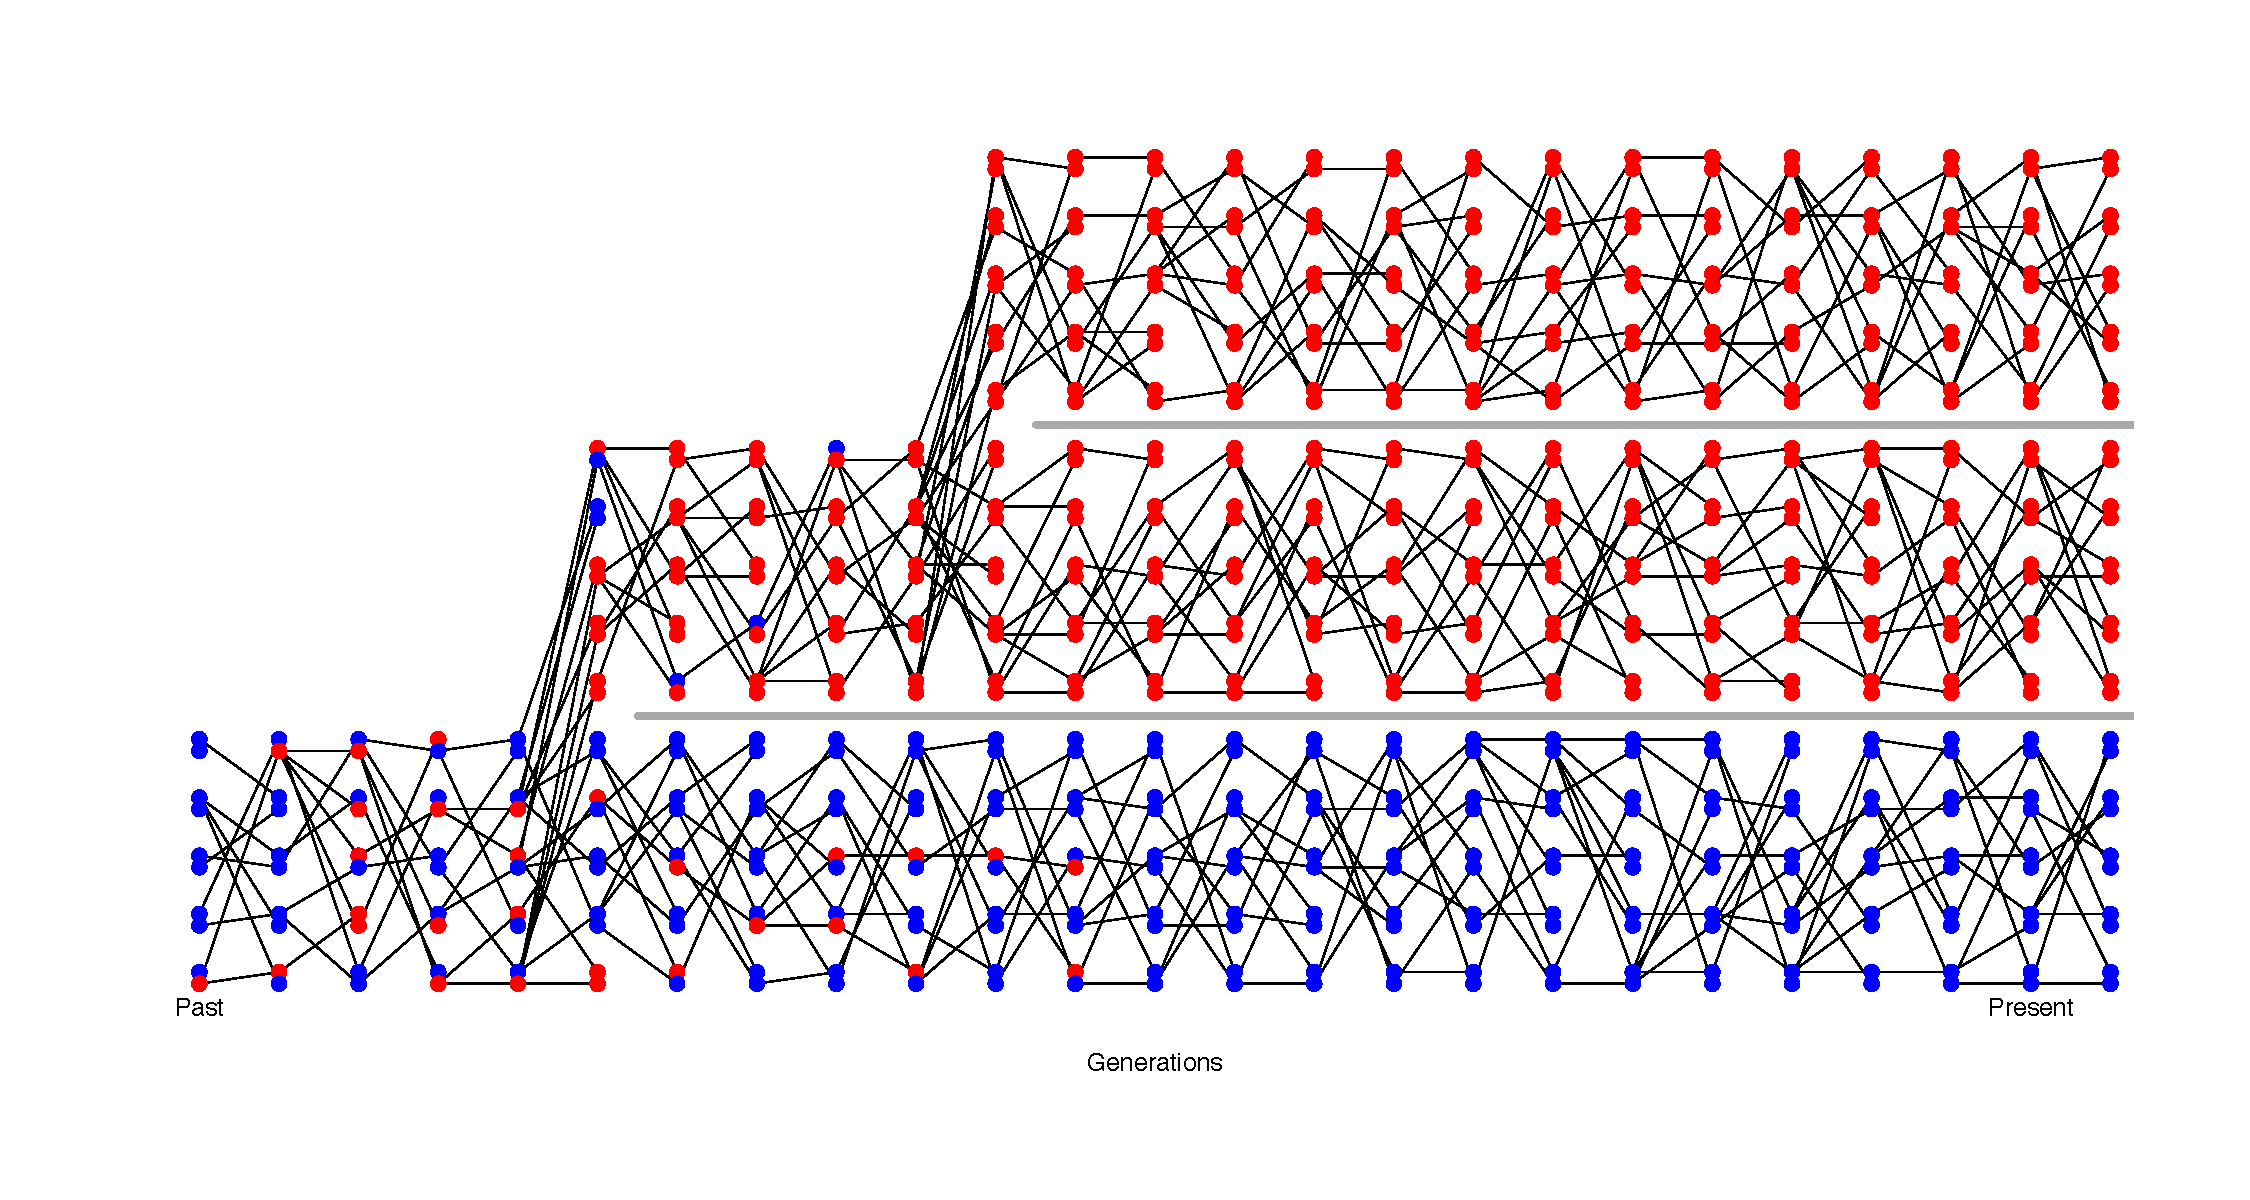
\includegraphics[width=\textwidth]{figures/Genetic_drift/ILS/no_ILS.pdf}
\end{center}
\caption{An example of alleles assorting among three populations such that there is no incomplete lineage sorting. \gitcode{https://github.com/cooplab/popgen-notes/blob/master/Rcode/Loss_of_heterozyg_varying_pop.R}} \label{fig:NoILS_poly} 
\end{figure}

\begin{figure}
\begin{center}
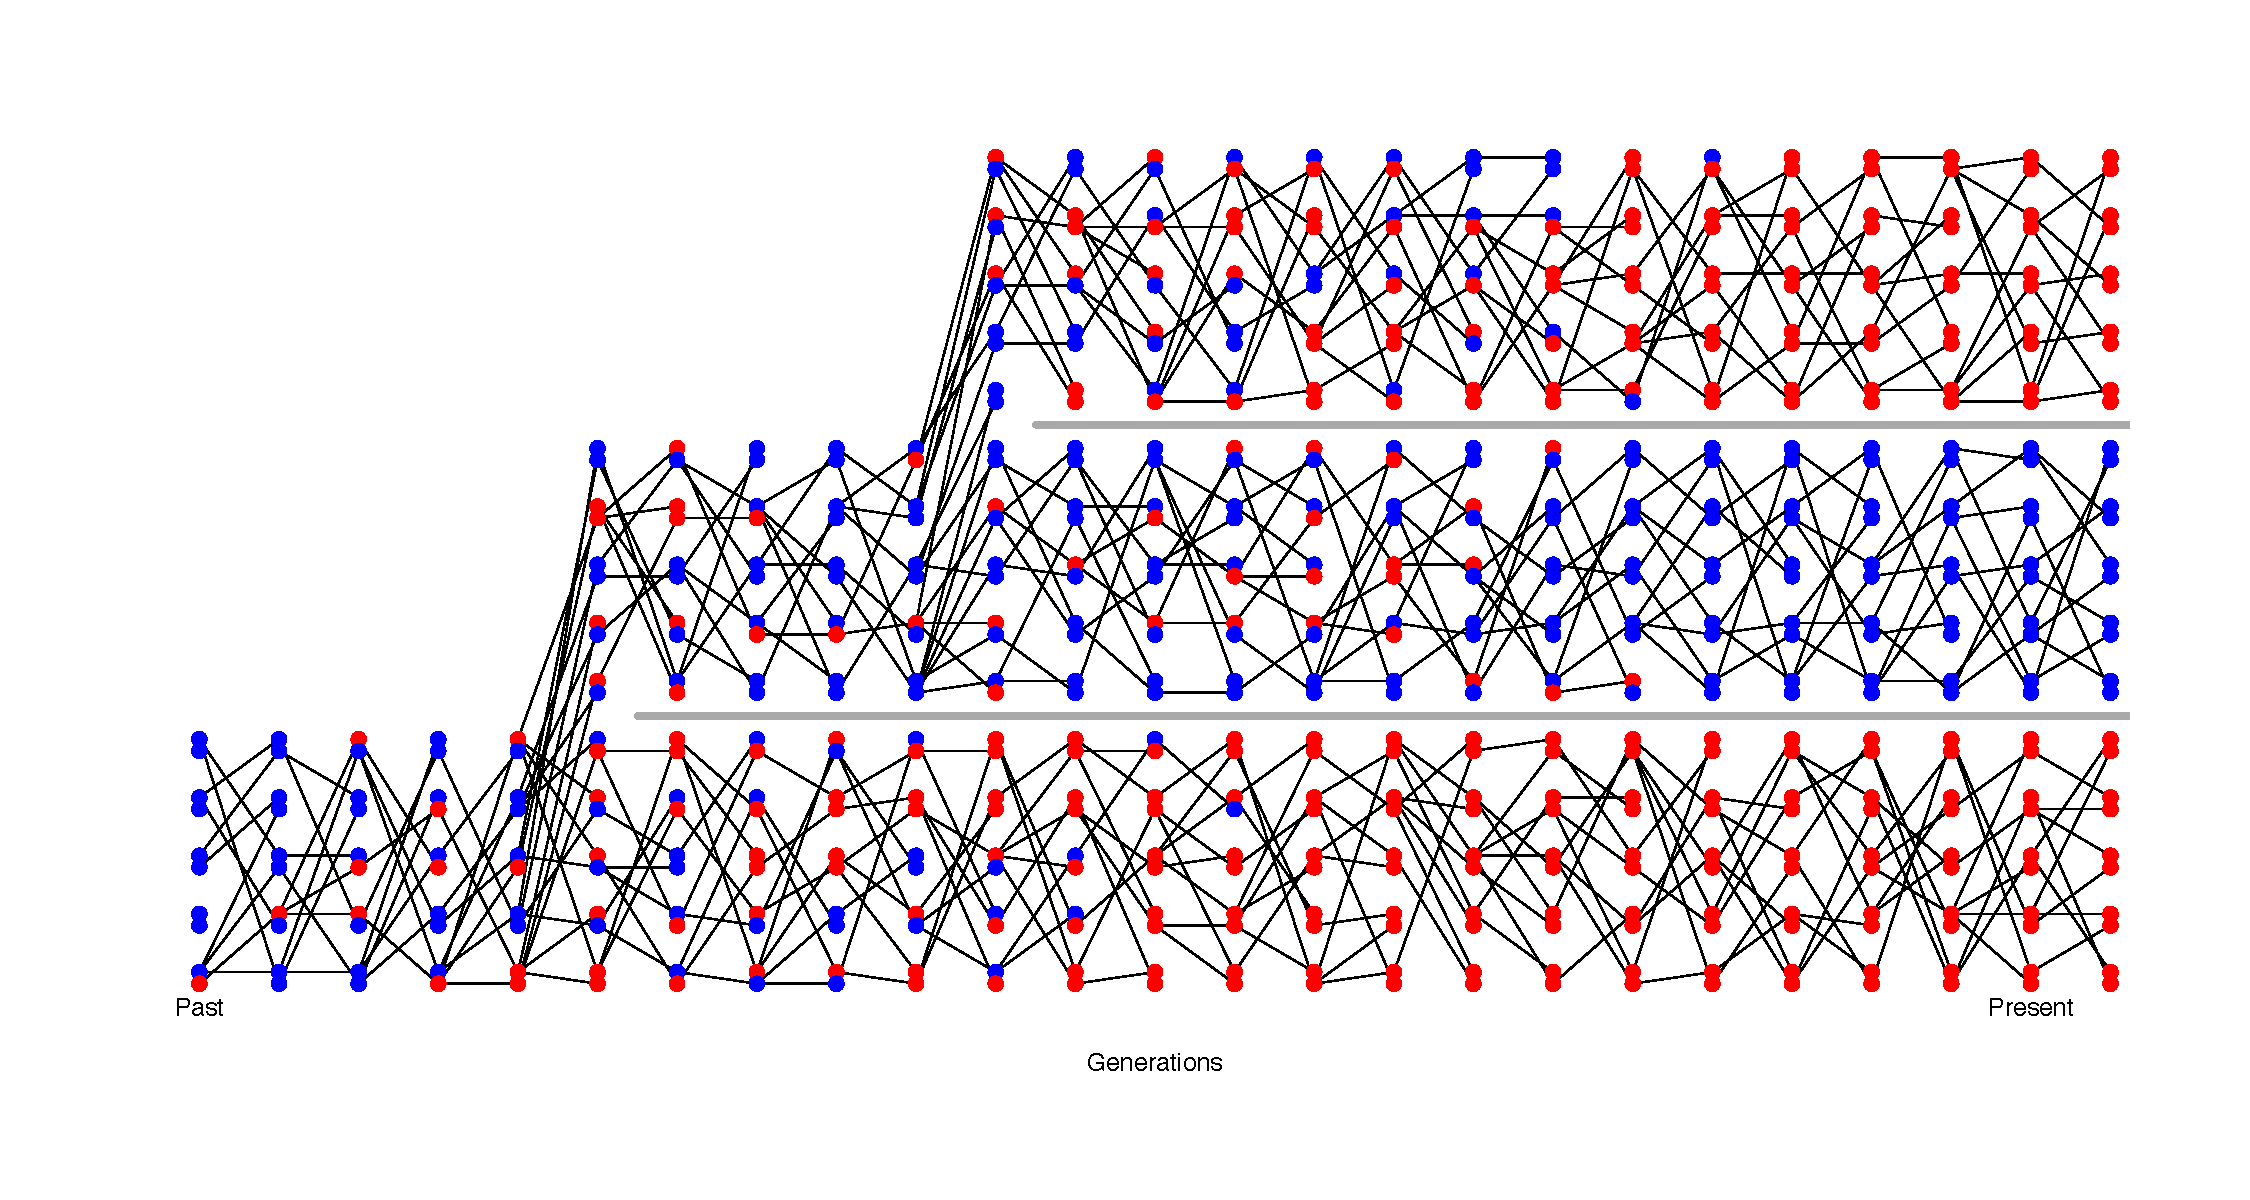
\includegraphics[width=\textwidth]{figures/Genetic_drift/ILS/ILS.pdf}
\end{center}
\caption{An example of alleles assorting among three populations leading to incomplete lineage sorting. \gitcode{https://github.com/cooplab/popgen-notes/blob/master/Rcode/Loss_of_heterozyg_varying_pop.R} } \label{fig:ILS_poly} 
\end{figure}


\begin{figure}
\begin{center}
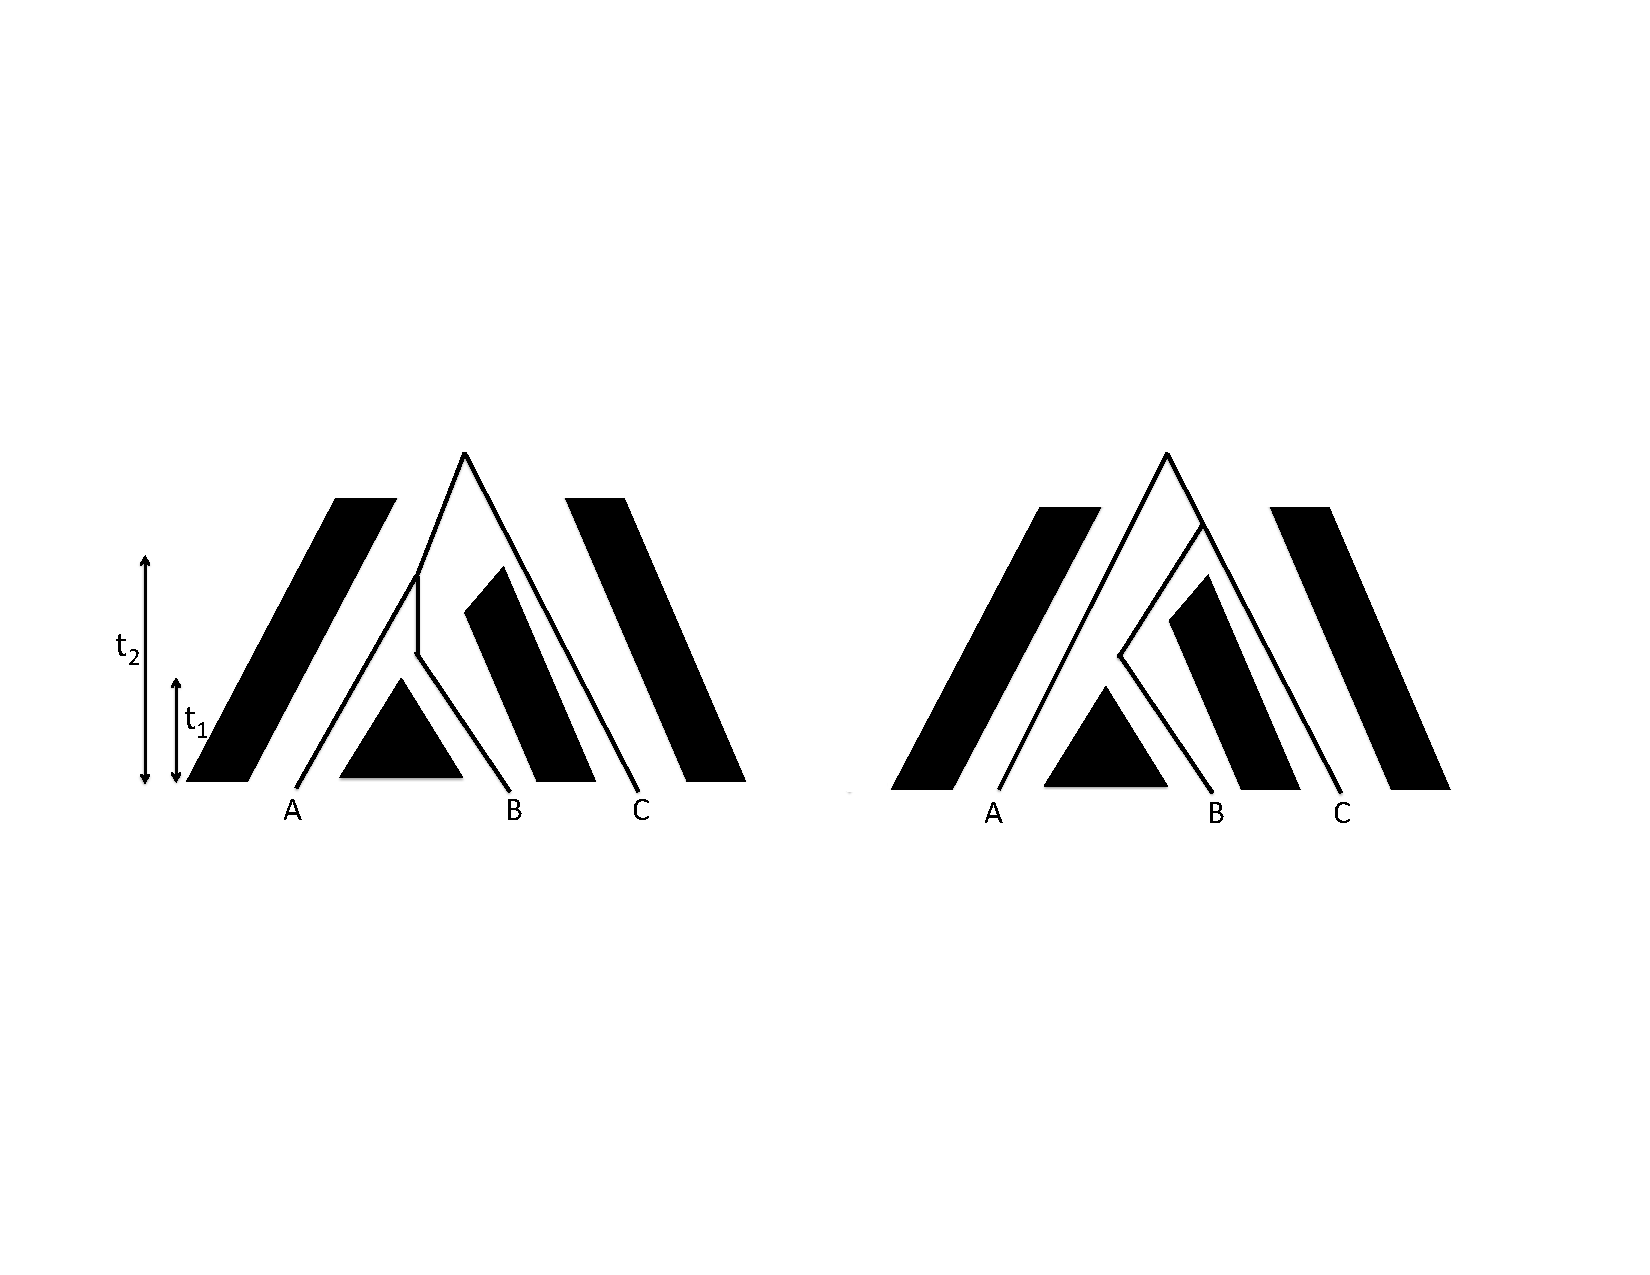
\includegraphics[width=\textwidth]{figures/Genetic_drift/ILS/ILS_coal_cartoon.pdf}
\end{center}
\caption{The population tree of three populations ((A, B), C) is shown
blocked out with black shapes. Two different coalescent trees are
relating a single allele drawn from A, B, and C are shown with thinner lines.} \label{fig:ILS_cartoon} 
\end{figure}

A natural pedigree analogy to incomplete lineage sorting is the fact that while two
biological siblings are more closely related to each other genealogically than
either is to their cousin, at any given locus one of the siblings can
share an allele IBD with their cousin that they do not share with
their own sibling, due to the randomness of Mendelian segregation down their
pedigree. In these cases, the average relatedness of the individuals/populations disagrees
with the patterns of relatedness at a particular locus. 


%\begin{question}
%Draw a pedigree of two full cousins, where one of the cousins has a full sibling. Label the four alleles in shared grandparents 1-4, and draw the situation where the cousins share 1 allele IBD, and the sibs share 0 alleles IBD. 
%\end{question}
%This analogy isn't perfect as full cousins dont share one parents, while all three of our populations share one ancestral, parental population far enough back. If we want to make this analogy more perfect we'd need to posit a bunch of inbreeding, but honestly drawinf that would make my head hurt a lot. 

\begin{marginfigure}
\begin{center}
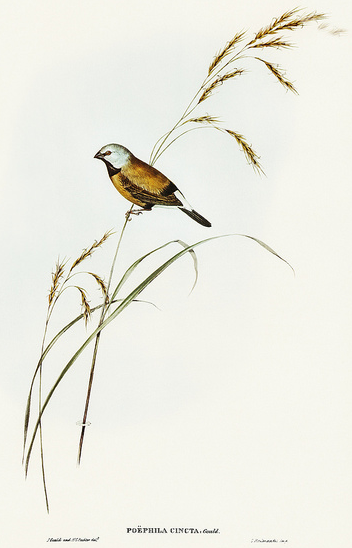
\includegraphics[width=\textwidth]{illustration_images/Genetic_drift/Poephila_cincta_finch/Poephila_cincta_finch.png}
\end{center}
\caption{Banded Grass Finch ({\it P. cincta}). Illustration by
  Elizabeth Gould.
  \newline \noindent \tiny{Birds of Australia Gould J. 1840. CC BY 4.0 uploaded to \href{https://www.flickr.com/photos/vintage_illustration/41073432105/in/photolist-WpHYmR-WBF2Uc-Uoq2kW-QAW9bN-UL33uh-RmyMxt-PKmBjN-8xpKmQ-8xmHg2-H6mfAS-dVREvC-7Qepuh-222xkPQ-7QepzS-25zw6ak-W28Nyk-Qa6d32-ijh2uH-6V8Srd-25zw5ov-8xpKB7-nUQ33T-6V8TLy-nV88oH-25RuYmq-21TcFz1-R2Gdy4-GdWRgi-GdMmry-GdWAwD-9mjwfA-25oHWeJ-HMbQre-6CQWTH-7TjKu-e6SYV-25RuXU3-pdKtxc-9hYCzE-voj7Sj-zqSdQb-6SNmDE-a1datx-a1dasZ-PFfPXY-rR7QYw-GJ7rey-6SJmuB-7TjFh}{Flickr} by \url{rawpixel.com}.}} \label{fig:Poephila_cincta} 
\end{marginfigure}

As an empirical example of incomplete lineage sorting, let's consider the work of 
\citeauthor{jennings:05} who sequenced a single allele from three
different species of Australian grass finches (Poephila): two sister species
of long-tailed finches ({\it Poephila acuticauda} and {\it P. hecki})
and the black-throated finch ({\it Poephila cincta}, see Figure \ref{fig:Poephila_cincta}). They collected
sequence data for 30 genes, and constructed phylogenetic gene trees
at each of these loci, resulting in 28 well-resolved gene trees. 
16 of the gene trees showed {\it
  P. acuticauda} and {\it P. hecki} as sisters with {\it P. cincta})
(the tree ((A,H),C)~), while for twelve genes the gene tree was
discordant with the population tree: for seven of their genes  {\it P. hecki}
fell as an outgroup to the other two and at five {\it P. acuticauda} fell as an outgroup (the trees ((A,C),H) and
((H,C),A) respectively). 


Let's use the coalescent to understand this discordance between gene
trees and species trees. Let's assume that two sister populations
(A \& B) split $t_1$ generations in the past, with a
deeper split from a third outgroup population (C) $t_2$ generations in the
past. We'll assume that there's no gene flow among our populations
after each split. We can trace back the ancestral lineages of our three alleles. The
first opportunity for the A \& B lineages to coalesce is $t_1$
generations ago. If they coalesce with each other in their shared
ancestral population before $t_2$ in the past (left side of
Figure \ref{fig:ILS_cartoon}) their gene tree will
definitely agree with the population tree. So the only way for the gene
tree to disagree with the population tree is for the A \& B lineages
to fail to coalesce in their shared ancestral population between $t_1$ and  $t_2$; this happens
with probability $\left(1 - \nicefrac{1}{2N}\right)^{t_2-t_1}$. We'll
get a discordant gene tree if A
\& B make it back to the shared ancestral population with C without
coalescing, and then one or the other of them coalesces with the C lineage before they coalesce with each other. This happens with probability $2/3$, as at the first
pairwise-coalescent event there are are three possible pairs of lineages that could coalesce, two of
which (A \& C  and B \$ C ) result in a discordant tree. So the
probability that we get a coalescent tree that is discordant with the population tree is
\begin{equation}
\frac{2}{3} \left(1 - \nicefrac{1}{2N}\right)^{t_2-t_1}.
\end{equation}
Thus we should expect gene-tree population-tree discordance when populations split in rapid succession and/or population sizes are large. 
\begin{question}
Let's return to \citeauthor{jennings:05}'s Australian grass finches
example. They estimated that the ancestral population size of our two
long-tailed finches was four hundred thousand. What is your best
estimate of the inter-speciation time, i.e. $t_2-t_1$? 
\end{question}

\paragraph{Testing for gene flow.} 

We often want to test whether gene flow has occurred between populations. For example, we might want to establish a case
that interbreeding between humans and Neanderthals occurred or demonstrate that
gene flow occurred after two populations began to speciate. 
A broad range of methods have been designed to test for gene flow and
to estimate gene flow rates, based on neutral expectations. Here we'll briefly just discuss one method based on
some simple coalescent ideas.  Above we assumed that gene-tree population-tree discordance was due to
incomplete lineage sorting due to populations rapidly
splitting. However, gene flow among populations can also lead to gene-tree discordance.
While both ILS and gene flow can lead to discordance, under
simplifying assumptions, ILS implies more symmetry in how these
discordances manifest themselves.\\


\begin{figure}
\begin{center}
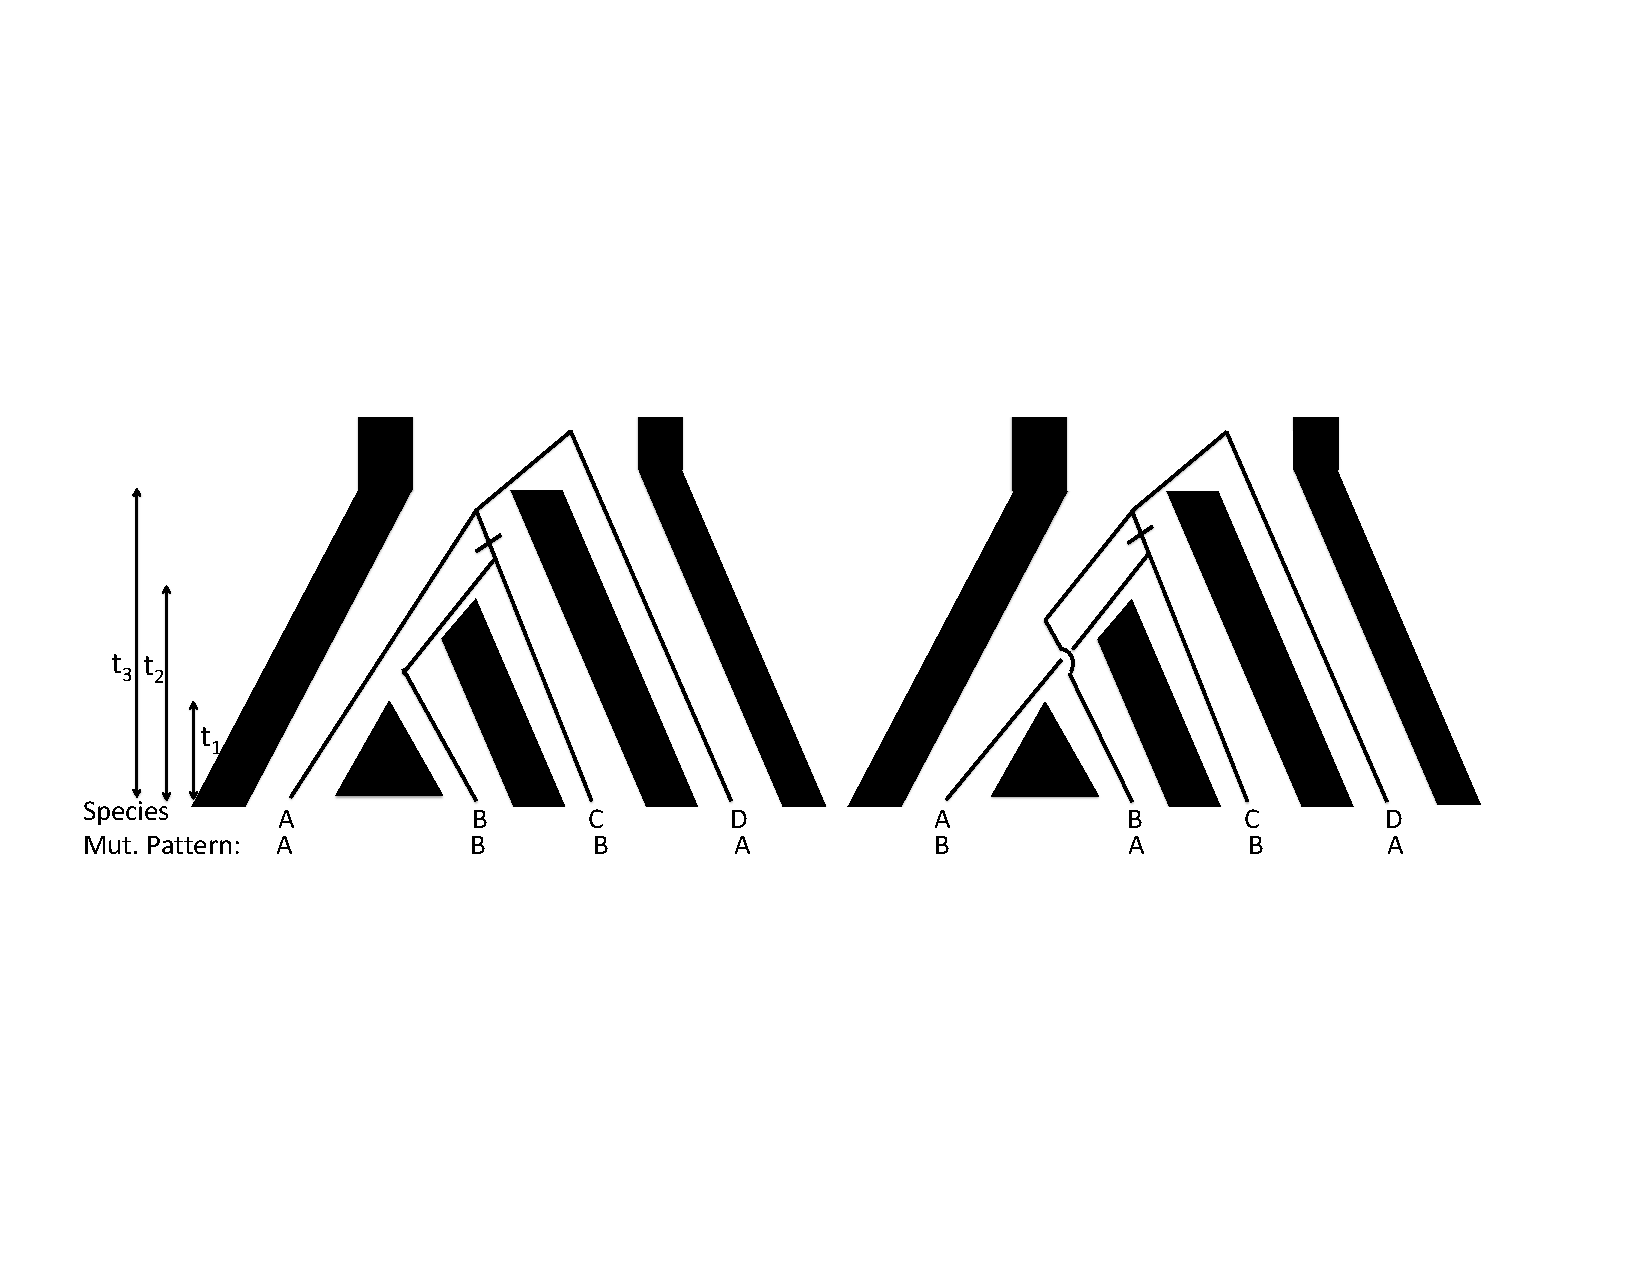
\includegraphics[width=\textwidth]{figures/Genetic_drift/ILS/ABBA_BABA_coal.pdf}
\end{center}
\caption{ In both the left and and right trees ILS has occurred between our single lineages sampled from populations A, B, and C. Imagine that population D is a somewhat distant outgroup
such that the lineages from A through C (nearly) always coalesce with each other before any coalesce with D. The small dash on the branch indicates the mutation A$\rightarrow$B occurring, giving rise to the
ABBA or BABA mutational pattern shown at the bottom. } \label{fig:ABBA_BABA} 
\end{figure}

Take a look at Figure \ref{fig:ABBA_BABA}. In both cases the lineages from A and B fail to coalesce in
their initial shared ancestral population, and one or the other of them
coalesces with the lineage from C before they coalesce with each other. Each option is equally
likely; therefore the mutational patterns ABBA and BABA are equally likely to occur under ILS.  \sidenote{here we have to assume no structure in the ancestral population.}

However, if gene flow occurs from population C into population B, in addition to ILS the lineage from B can more recently coalesce with the lineage from C, and so we should see more ABBAs than BABAs. To test for this effect of gene flow, we can sample a sequence from each of our 4 populations and count up the number of sites that show the two mutational patterns consistent with the gene-tree discordance $n_{ABBA}$ and
$n_{BABA}$ and calculate
\begin{equation}
\frac{n_{ABBA}-n_{BABA}}{n_{ABBA}+n_{BABA}}
\end{equation}
This statistic will have expectation zero if the gene-tree discordance is due to ILS and will be skewed negative if gene flow
occurred from C into B (and skewed positive if gene flow occurred from C into A).
\graham{Add ABABA BABA egs}
